\documentclass[utf8x,usehyperref,14pt]{G7-32}
\usepackage[T2A]{fontenc}
\usepackage[utf8x]{inputenc} %% ваша любимая кодировка здесь
\usepackage[english,russian]{babel} %% это необходимо для включения переносов
\usepackage{float}
\usepackage[pdftex]{graphicx}
\TableInChaper % таблицы будут нумероваться в пределах раздела
\PicInChaper   % рисунки будут нумероваться в пределах раздела
\setlength\GostItemGap{2mm}% для красоты можно менять от 0мм
% \bibliographystyle{unsrt} %Стиль библиографических ссылок БибТеХа
\sloppy
\usepackage{array}
\bibstyle{utf8gost705u}
\renewcommand{\theequation}{(\arabic{chapter}.\arabic{equation})} 
\makeatletter
\@addtoreset{equation}{chapter} % Счетчик формул
\makeatother
%\bibliographystyle{unsrt}
%%%%%%%<------------- НАЧАЛО ДОКУМЕНТА
\setcounter{page}{3}
\begin{document}
%\usefont{T2A}{ftm}{m}{} %%% Использование шрифтов Т2 для возможности скопировать текст из PDF-файлов.
%\frontmatter %%% <-- это выключает нумерацию ВСЕГО; здесь начинаются ненумерованные главы типа Исполнители, Обозначения и прочее
%\NirTitle{\textbf{<<Торсионные наногенераторы плазменных стволовых клеток с протонной накачкой>>}}

%\Introduction
%\mainmatter %% это включает нумерацию глав и секций в документе ниже
\tableofcontents

\chapter{Работа \No1. Знакомство со средой разработки IAR Embedded Workbench for ARM (EWARM). Разработка программы с использованием библиотеки Standard Peripherals Library (SPL)}
Цель работы: 
\begin{itemize}
\item Знакомство со средой разработки IAR.
\item Изучение принципов работы со светодиодами, знакомство со Standard Peripherals Library (SPL).
\item Изучение принципов отладки программы в среде IAR.
\end{itemize}
\section{Обзор платы STM32L-Discovery}
В данной работе используется отладочная плата STM32L - Discovery на базе 32 МГц микроконтроллера STM32L152RB с 128 KБ Flash, 16 KБ RAM и 4 KБ EEPROM от STMicroelectronics.  Микроконтроллер построен на основе ядра Cortex-M3. Данные микроконтроллеры отличаются ультранизким энергопотреблением (порядка 270 нА в спящем режиме). STM32L-Discovery --- полноценный инструментарий, включающий в себя отладочную плату, программатор и отладчик с поддержкой самых популярных программных средств разработки от таких фирм как IAR, Keil и Atollic. Сигналы встроенного программатора-отладчика ST-Link выведены на внешний разъем, что позволяет в дальнейшем использовать STM32L-Discovery в качестве программатора-отладчика для своих собственных разработок.

Основные характеристики STM32L-Discovery:
\begin{itemize}
\item Микроконтроллер STM32L152RBT6
\item Ядро Cortex-M3, 128 KB Flash, 16 KB RAM, 4 KB EEPROM
\item Интерфейсы USB 2.0 FS, 3xUSART, 2xSPI, 2xI2C, 8 таймеров
\item 24-канальный 12-бит АЦП, компараторы, 2х12-бит ЦАП
\item Полноценные часы реального времени
\item Встроенный контроллер LCD 8х40
\item Встроенный программатор ST-Link с возможностью программировать другие микроконтроллеры STM32.
\item LCD дисплей 24х8 в форм-факторе DIP28
\item Возможность измерения потребляемого тока
\item Четыре светодиода:
\begin{itemize}
\item LD1 (красный/зеленый) для сигнализации обмена данных по USB
\item LD2 (красный) для питания 3.3В
\item Два пользовательских диода LD3 (зеленый) и LD4 (синий)
\end{itemize}
\item Две кнопки (user и reset)
\item Сенсорная клавиатура (четыре сенсорных кнопки или один слайдер)
\item Все свободные выводы STM32L152RBT6 выведены на контактные площадки
\end{itemize}

Летом 2013 года появилась отладочная плата STM32L152C-DISCO из линейки DISCOVERY на базе микроконтроллера STM32L152RCT6, который отличается от STM32L152RB большим объемом памяти: 256 КБ Flash-памяти, 32 КБ ОЗУ и 8 КБ EEPROM.



\section{Общие сведения о ядре Cortex}

Семейство ARM Cortex --- новое поколение процессоров, которые выполнены по стандартной архитектуре. В отличие от других процессоров ARM, семейство Cortex является завершенным процессорным ядром. 

Семейство Cortex доступно в трех основных профилях: 
\begin{itemize}
\item \textit{Cortex-A} --- для высокопроизводительных применений. Это полноценные процессоры общего назначения для самых различных задач. Процессор Apple A5, используемый в iPhone 4S и iPad 2, построен на основе ядра Cortex-A9.
\item \textit{Cortex-R} --- профиль для операционных систем реального времени (ОСРВ, англ. Real-Time Operating System).
\item \textit{Cortex-M} --- для чувствительных к стоимости и микроконтроллерных применений. 
\end{itemize}

Для упрощение разработки под микроконтроллер используется \textit{CMSIS (Cortex Microcontroller Software Interface Standard)}. \textit{CMSIS} --- уровень абстракции аппаратного обеспечения для Cortex-M, обеспечивающий последовательный и простой интерфейс программного обеспечения для процессора и периферийных устройств. \textit{CMSIS} стандартизирует программное обеспечение, позволяя переносить его на другие устройства Cortex-M. 

CMSIS состоит из нескольких файлов:
\begin{itemize}
\item \textit{core\_cm3.c, core\_cm3.h}\footnote{IAR, начиная с версии 6.2, использует собственные файлы core\_cm3.c, core\_cm3.h} --- описание ядра, стандартизировано для всех Cortex-M3.
\item \textit{stm32l1xx.h} --- файл описание периферии, а также структуры доступа к ним. 
\item \textit{system\_stm32l1xx.c} --- функции CMSIS. 
\item \textit{system\_stm32l1xx.h} --- заголовочные файлы для функций CMSIS.
\end{itemize}

CMSIS доступен на сайте производителя микроконтроллеров.


\section{Создание проекта в IAR}

IAR EWARM --- интегрированная среда разработки, включающая в себя компилятор языка Си, отладчик (debugger) и компоновщик (linker). Создание программного обеспечения для микроконтроллера подразумевает создание проекта, который будет объединять CMSIS, сторонние библиотеки и исходные коды на языке Си. Для создание нового проекта нужно выбрать:
\begin{center}
\textit{Project => Create New Project}
\end{center}


\begin{figure}[h!]
\begin{center}
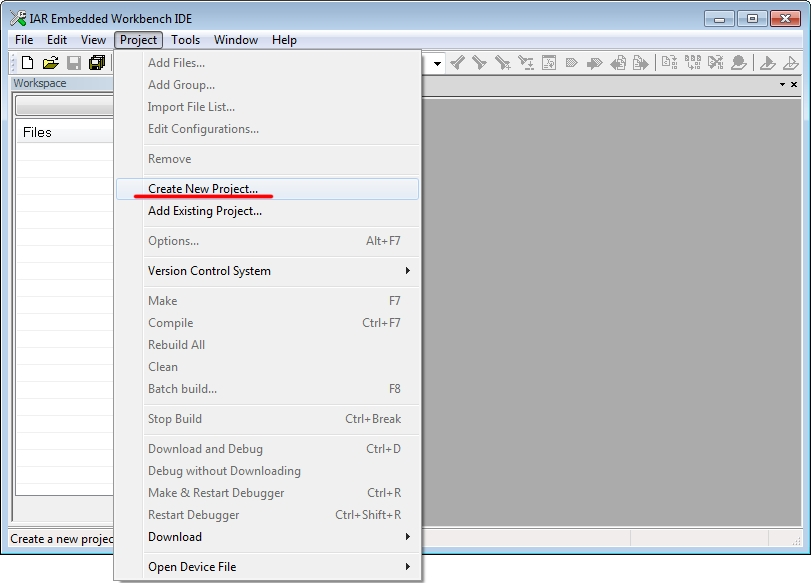
\includegraphics[scale=0.5]{Image/4_1}
\end{center}
\caption{Создание нового проекта}
\end{figure}

В появившемся окне можно выбрать язык программирования. В данной лабораторной это язык Си. Подпункт \textit main позволяет создать файл главной программы \textit{main.c} вместе с каркасом функции \verb\main()\.

\begin{verbatim}
int main()
{
  return 0;
}
\end{verbatim}



\begin{figure}[h!]
\begin{center}
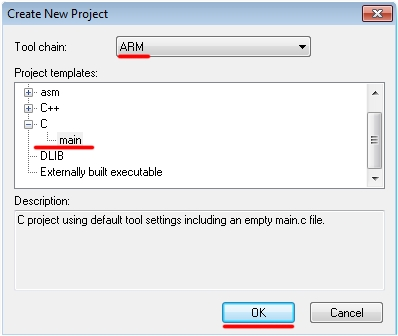
\includegraphics[scale=0.6]{Image/5.jpg}
\end{center}
\caption{Выбор языка программирования}
\end{figure}


Файлы внутри проекта можно объединять в группы (папки, подпапки).  Для упрощения работы с периферией существуют библиотеки \textit{Standard Peripherals Library (SPL)}. В данной работе потребуются библиотека для работы с \textit{GPIO (General Purpose Input-utput)} -- портами ввода-вывода общего назначения и библиотека для работы с \textit{RCC (Reset and Clock Control)} -- системой тактирования и сброса. Создайте группу \textit{SrdPereph}, в ней подпапки \textit{inc} -- для заголовочных файлов, \textit{src} -- для исходных файлов.

\begin{figure}[h!]
\begin{center}
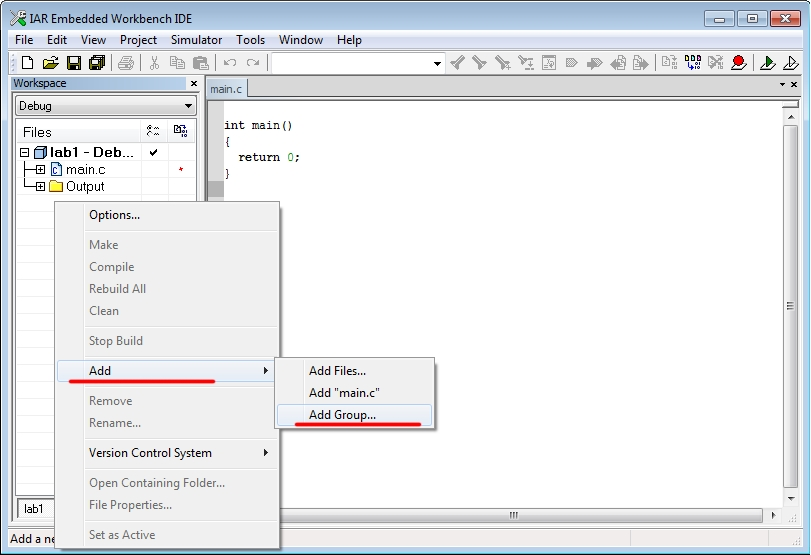
\includegraphics[scale=0.5]{Image/6.jpg}
\end{center}

\caption{Создание новой группы}
\end{figure}

Добавьте в созданные папки файлы библиотек \verb\stm32l1xx_gpio.h\, \verb\stm32l1xx_gpio.с\, \verb\stm32l1xx_rcc.c\, \verb\stm32l1xx_rcc.h\ из папки \verb\STM32L1xx_StdPeriph_Driver\.


\begin{figure}[h!]
\begin{center}
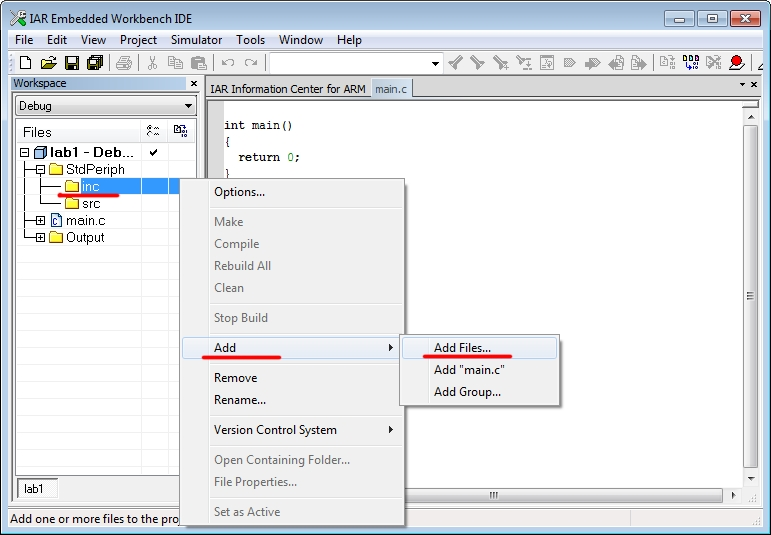
\includegraphics[scale=0.5]{Image/7.jpg}
\end{center}
\caption{Добавление файлов библиотек}
\end{figure}

Для дальнейшей работы необходимо настроить проект под заданный микроконтроллер.

\begin{figure}[h!]
\begin{center}
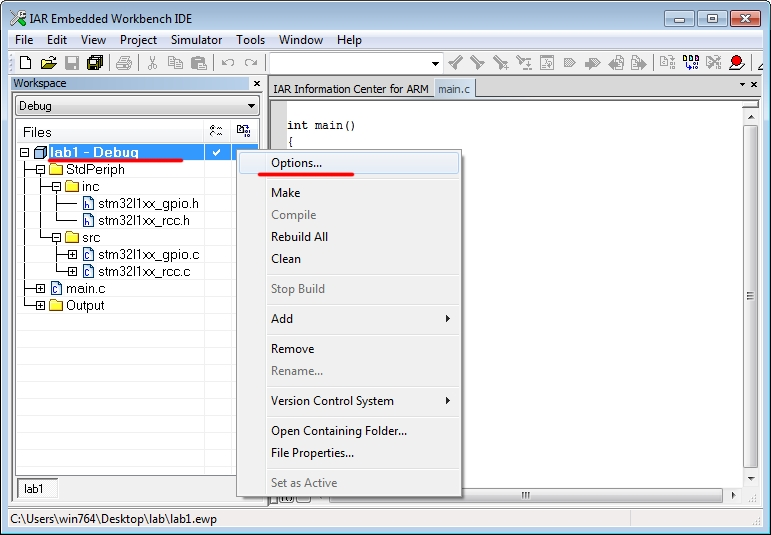
\includegraphics[scale=0.5]{Image/8.jpg}
\end{center}
\caption{Настройка проекта}
\end{figure}

В категории  \textit{ General Options}, во вкладке \textit{Target}, отметьте пункт \textit{Device} и в выпадающем списке выберите микроконтроллер 
\begin{center}
\textit{ST => ST ST32L52xB}
\end{center}

\begin{figure}[H]
\begin{center}
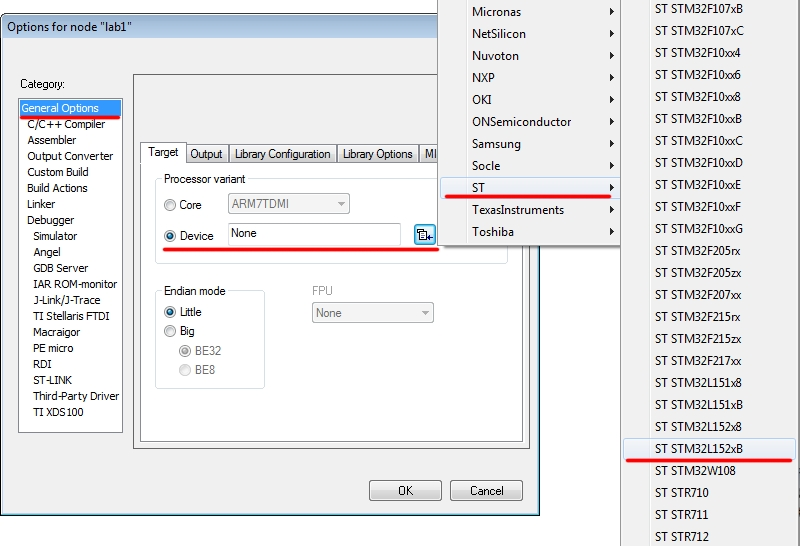
\includegraphics[scale=0.5]{Image/9.jpg}
\end{center}
\caption{Выбор микроконтроллера}
\end{figure}

В категории \textit{General Options}, во вкладке \textit{Library Configuration}, в выпадающем списке \textit{Library} выберите \textit{Full} -- для полного использования библиотеки времени выполнения (runtime library). Отметьте пункт \textit{Use CMSIS} для использования файлов описания ядра, разработанных IAR.


\begin{figure}[h!]
\begin{center}
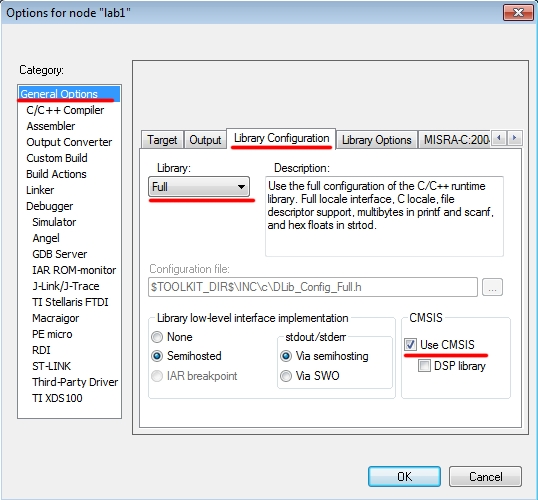
\includegraphics[scale=0.5]{Image/10.jpg}
\end{center}
\caption{Настройка библиотек}
\end{figure}

В категории  \textit{ C/C++ Compiler}, во вкладке \textit{Preprocessor} необходимо указать компилятору пути до заголовочных файлов.
Для относительного описания пути можно использовать переменную \verb\$PROJ_DIR$\ -- директория\ проекта.
\begin{verbatim}
$PROJ_DIR$\STM32L1xx_StdPeriph_Driver\inc
$PROJ_DIR$\CMSIS\CM3\DeviceSupport\ST\STM32L1xx
$PROJ_DIR$\
\end{verbatim}
Иногда принято размещать CMSIS и библиотеки переферии в одном месте, прописывая в настройках проекта абсолютный путь вида: \verb#C:\Library\CMSIS#, а не использовать локальную копию файлов библиотеки в каждом проекте.


\begin{figure}[H]
\begin{center}
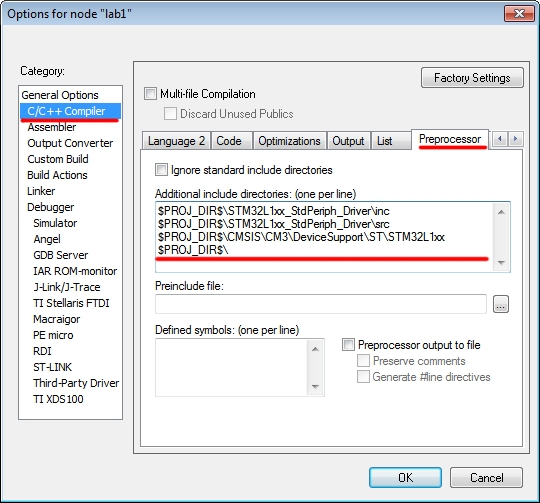
\includegraphics[scale=0.5]{Image/11.jpg}
\end{center}

\caption{казание дополнительных путей до файлов}
\end{figure}

По умолчанию IAR генерирует исполняемый файл в формате  \textit{ELF (Executable and Linkable Format)} -- формат исполняемых и компонуемых файлов, используемый во многих UNIX-подобных операционных системах. При желании, можно выбрать дополнительный формат. В категории  \textit{Output Converter} отметьте пункт  \textit{Generate additional output}, а в выпадающем списке  \textit{Output format} выберете  \textit{binary}.

\begin{figure}[H]
\begin{center}
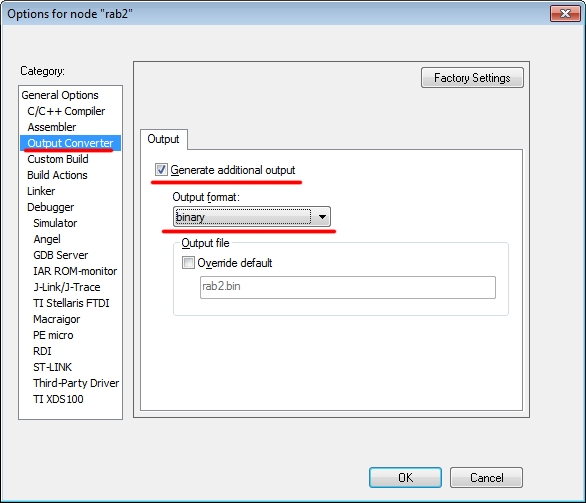
\includegraphics[scale=0.5]{Image/12.jpg}
\end{center}
\caption{Выбор формата исполняемого файла}
\end{figure}

В категории \textit{Linker}, отметьте пункт \textit{Override default} (отменить настройки по умолчанию), нажмите \textit{Edit} для настройки конфигурации компоновщика.


\begin{figure}[h!]
\begin{center}
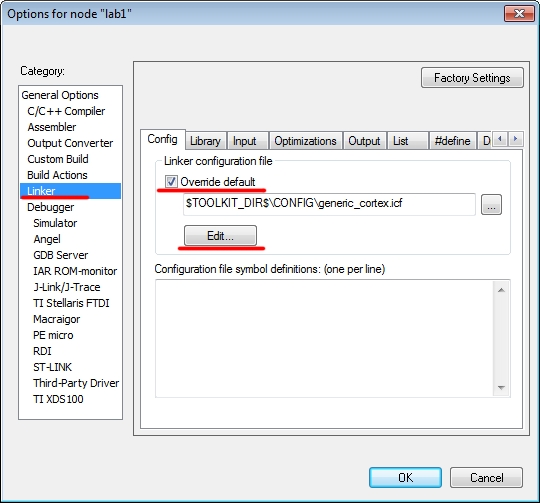
\includegraphics[scale=0.5]{Image/13.jpg}
\end{center}
\caption{Указание дополнительных путей до файлов}
\end{figure}

Во вкладке \textit{Vector Table} необходимо указать начало таблицы векторов прерываний. Адрес может быть \verb\0x00000000\ или \verb\0x08000000\. Адрес \verb\0x08000000\ указывает на начало внутренней Flash памяти, так же этот адрес рекомендует использовать STMicroelectronics в своем руководстве \textit{UM1451 User manual}. 


\begin{figure}[h!]
\begin{center}
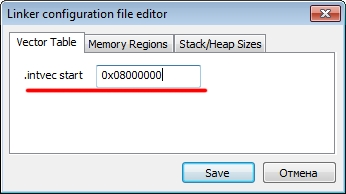
\includegraphics[scale=0.7]{Image/14.jpg}
\end{center}
\caption{Указание начала таблицы векторов прерываний}
\end{figure}

Во вкладке \textit{Memory Regions} задаются адреса начала и окончания ROM (ПЗУ) и RAM (ОЗУ). ROM -- внутренняя Flash память, начинается с адреса \verb\0х08000000\. Адрес окончания у каждого микроконтроллера разный и зависит от объема Flash памяти. Адрес окончания рассчитывается по формуле:

\begin{center}
	\[Адрес_{16} = адрес\ начала_{16} + размер\ Flash\ памяти_{16}-1_{16}\]
\end{center}

В микроконтроллере STM32L152RB 128 КБ Flash памяти, 16 КБ RAM.

\begin{center}
	\[0x08000000+(128\cdot1024)_{10}-1_{16}=0x0801FFFF\]
\end{center}

RAM память начинается с адреса \verb\0x20000000\. Адрес окончания рассчитывается аналогично:

\begin{center}
	\[0x20000000+(16\cdot1024)_{10}-1_{16}=0x20003FFF\]
\end{center}
STMicroelectronics, в своем руководстве \textit{UM1451 User manual}, рекомендует использовать адрес \verb\0x20004000\, т.е. \verb\0x20003FFF + 1\
\begin{figure}[H]
\begin{center}
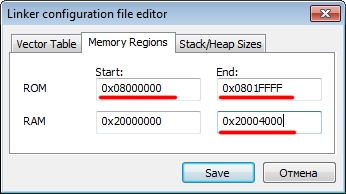
\includegraphics[scale=0.7]{Image/15.jpg}
\end{center}
\caption{Указание адреса начала и окончания ROM (ПЗУ) и RAM (ОЗУ)}
\end{figure}


В категории \textit{Debugger}, во вкладке \textit{Setup}, в выпадающем списке \textit{Driver} выберете \textit{ST-LINK}. Отметьте пункт \textit{Run to} и укажите значение \textit{main}, указывающее, что программа должна начинать работать с функции \textit{main}.



\begin{figure}[h!]
\begin{center}
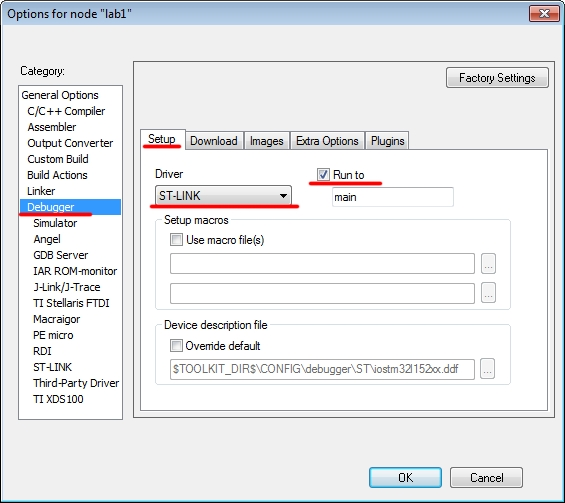
\includegraphics[scale=0.5]{Image/16.jpg}
\end{center}
\caption{Настройка отладчика. Часть 1}
\end{figure}

Во вкладке \textit{Download}, отметьте пункт \textit{Use flash loader(s)}, позволяющий программировать Flash непосредственно из среды IAR.


\begin{figure}[h!]
\begin{center}
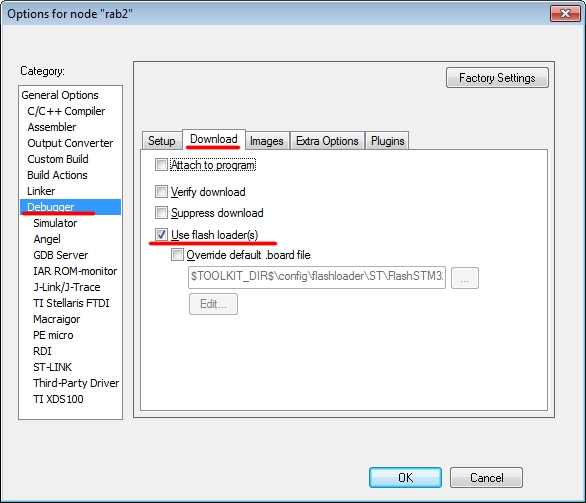
\includegraphics[scale=0.5]{Image/17.jpg}
\end{center}
\caption{Настройка отладчика. Часть 2}
\end{figure}

Для настройки встроенного программатора-отладчика\footnote{Программатор --- аппаратно-программное устройство, предназначенное для записи/считывания информации в постоянное запоминающее устройство} в категории \textit{ST-LINK}, в качестве интерфейса, выберете пункт \textit{SWD}.

\begin{figure}[h!]
\begin{center}
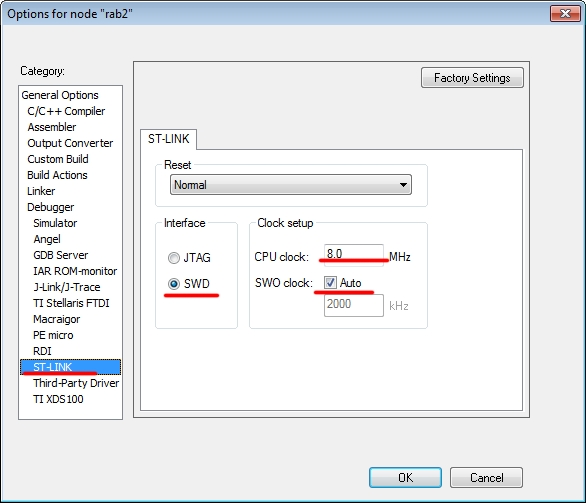
\includegraphics[scale=0.5]{Image/18.jpg}
\end{center}
\caption{Настройка программатора}
\end{figure}

При попытке собрать файлы проекта будет появляться ошибка:
\begin{verbatim}
Warning[Pe223]: function "assert_param" declared implicitly 
C:\EXAMPLES\lab1\stm32l1xx_gpio.c 124
\end{verbatim}

Ошибка указывает на то, что функция \textit{assert\_param()}, которая используется в библиотеке проверки своих аргументов, объявлена неявно. Для устранения ошибки создайте файл \verb\stm32l1xx_conf.h\ содержащий:

\begin{verbatim}
#ifndef STM32L1XX_CONF_H_
#define STM32L1XX_CONF_H_
/* ------------------- */
#ifndef USE_FULL_ASSERT
 #define assert_param(x)
#endif
/* ------------------- */
#endif
\end{verbatim}

Поместите файл в директорию проекта и добавьте его в проект. В исходные файлы подключаемых библиотек (\verb\stm32l1xx_rcc.c\, \verb\stm32l1xx_gpio.c\) добавьте строку:

\begin{verbatim}
#include <stm32l1xx_conf.h>
\end{verbatim}

Для сборки файлов проекта нажмите \textit{ Make} (F7). Будут созданы исполняемые файлы, в окне сообщений отобразиться количество ошибок и предупреждений.

\begin{figure}[H]
\begin{center}
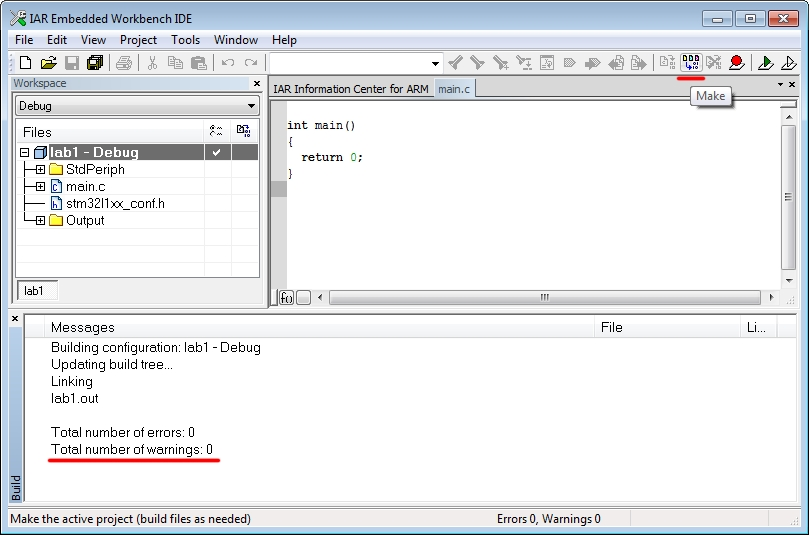
\includegraphics[scale=0.6]{Image/19.jpg}
\end{center}
\caption{Сборка файлов проекта}
\end{figure}


\subsection{Работа с периферией. Функции и структуры}
Для работы с периферией существуют два способа: Первый способ заключается в использовании регистров определенных в заголовочном файле \verb\stm32l1xx.h\ библиотеки CMSIS, расположенному в \verb#CMSIS/DeviceSupport/ST/STM32L1xx#. Для записи в регистр используются битмаски или шестнадцатеричные коды. Программирование через регистры достаточно трудно, но позволяет добиться большей производительности. Программирование с использованием регистров будет описано во второй лабораторной работе

Второй способ заключается в использовании готовых библиотек, например,\textit{ Standard Peripherals Library (SPL)} или \textit{Touch-Sensing Library (TSL)}. Библиотеки предоставляют готовые функции для работы с периферией, однако, скорость выполнения программы снижается, поскольку, в конечном итоге, все библиотечные функции управляют периферией через регистры. 

В данной лабораторной работе управление периферией (светодиодами) будет происходить через библиотеку \textit{Standard Peripherals Library (SPL)}, все необходимые для этого функции находятся в файлах \verb\stm32l1xx_gpio.h\, \verb\stm32l1xx_rcc.h\ в папке \verb#LabWorkSTM32L/Materials/STM32L1xx_StdPeriph_Driver#.

Светодиод \textit{LD3} подключен к порту ввода-вывода \textit{PB7}, светодиод \textit{LD4} подключен к порту ввода-вывода \textit{PB6}. По умолчанию периферия STM32 не работает, пока на нее не подан тактирующий сигнал. Для подачи тактирующего сигнала используется функция, прототип которой объявлен в заголовочном файле \verb\stm32l1xx_rcc.h\:
\begin{verbatim}
void RCC_AHBPeriphClockCmd(uint32_t RCC_AHBPeriph, 
                           FunctionalState NewState);
\end{verbatim}


Где \textit{AHB} --- шина, от которой происходит тактирование. Определить нужную шину можно по названию именованной константы в файле  \verb\stm32l1xx_rcc.h\:
\begin{verbatim}
...
#define RCC_AHBPeriph_GPIOA       RCC_AHBENR_GPIOAEN
#define RCC_AHBPeriph_GPIOB       RCC_AHBENR_GPIOBEN
#define RCC_AHBPeriph_GPIOC       RCC_AHBENR_GPIOCEN
#define RCC_AHBPeriph_GPIOD       RCC_AHBENR_GPIODEN
#define RCC_AHBPeriph_GPIOE       RCC_AHBENR_GPIOEEN
...
\end{verbatim}
Или на функциональной схеме, приведенной на рисунке 

\begin{Huge}
===================================

ФУНКЦИОНАЛЬНАЯ СХЕМА

===================================
\end{Huge}


В качестве первого аргумента функции используется приведенная выше именованная константа \verb\RCC_AHBPeriph_GPIOB\ (В случае портов PB6, PB7). В качестве второго аргумента используется константа перечисляемого типа \verb\ENABLE\ или \verb\DISABLE\, определенная в файле \verb\stm32l1xx.h\:

\begin{verbatim}
typedef enum {DISABLE = 0, ENABLE = !DISABLE} FunctionalState;
\end{verbatim}
Таким образом, функция для подачи тактирующего сигнала на порты GPIOB примет вид:
\begin{verbatim}
RCC_AHBPeriphClockCmd(RCC_AHBPeriph_GPIOB, ENABLE);
\end{verbatim}

Для описания режимов работы порта необходимо объявить переменную структурного типа \verb\GPIO_InitTypeDef\, которая содержит настройки порта в качестве полей структуры. Структура описывается в заголовочном файле периферии, которую необходимо инициализировать. В данной работе используются GPIO, следовательно, информация о структуре находиться в файле \verb\stm32l1xx_gpio.h\:
\begin{verbatim}
typedef struct
{
uint32_t GPIO_Pin;            /*!< Specifies the GPIO pins to be 						  
                              configured. This parameter can be any 					       
                              value of @ref GPIO_pins_define */

GPIOMode_TypeDef GPIO_Mode;   /*!< Specifies the operating mode for 						   
                              the selected pins. This parameter can 						   
                              be a value of @ref GPIOMode_TypeDef */

GPIOSpeed_TypeDef GPIO_Speed; /*!< Specifies the speed for the 						    
                              selected pins. This parameter can be a 					    
                              value of @ref GPIOSpeed_TypeDef */

GPIOOType_TypeDef GPIO_OType; /*!< Specifies the operating output 						    
                              type for the selected pins. This 						    
                              parameter can be a value of @ref 						    
                              GPIOOType_TypeDef */

GPIOPuPd_TypeDef GPIO_PuPd;   /*!< Specifies the operating Pull-						    
                              up/Pull down for the selected pins. 						    
                              This parameter can be a value of @ref 					    
                              GPIOPuPd_TypeDef */
}GPIO_InitTypeDef;
\end{verbatim}

Поля структуры имеют типы, определенные в качестве перечислений (enum) в файле \verb\stm32l1xx_gpio.h\:
\begin{verbatim}
typedef enum
{ 
  GPIO_Speed_400KHz = 0x00, /*!< Very Low Speed */
  GPIO_Speed_2MHz   = 0x01, /*!< Low Speed */
  GPIO_Speed_10MHz  = 0x02, /*!< Medium Speed */
  GPIO_Speed_40MHz  = 0x03  /*!< High Speed */
}GPIOSpeed_TypeDef;
...
typedef enum
{ 
  GPIO_Mode_IN   = 0x00, /*!< GPIO Input Mode */
  GPIO_Mode_OUT  = 0x01, /*!< GPIO Output Mode */
  GPIO_Mode_AF   = 0x02, /*!< GPIO Alternate functionMode */
  GPIO_Mode_AN   = 0x03  /*!< GPIO Analog Mode */
}GPIOMode_TypeDef;
...
\end{verbatim}
В данной работе структура будет иметь следующий вид:
\begin{verbatim}
GPIO_InitTypeDef Имя_структуры;
Имя_структуры.GPIO_Pin = GPIO_Pin_7 | GPIO_Pin_6 ; 
Имя_структуры.GPIO_Mode = GPIO_Mode_OUT;
Имя_структуры.GPIO_Speed = GPIO_Speed_2MHz;
Имя_структуры.GPIO_OType = GPIO_OType_PP;
\end{verbatim}

\verb\GPIO_Mode_OUT\ -- указывает, что порт является выходом. В случае если не указать тип в структуре, то при подаче питания на отладочную плату порт будет находиться в произвольном состоянии.

\verb\GPIO_OType_PP\ -- указывает, что выход имеет два состояния (Push-Pull) -- двухтактный полноценный выход или 0 или 1.

Для портов используется функция, прототип которой объявлен в заголовочном файле \verb\stm32l1xx_gpio.h\:
\begin{verbatim}
void GPIO_Init(GPIO_TypeDef* GPIOx, GPIO_InitTypeDef* GPIO_InitStruct);
\end{verbatim}
В качестве аргументов функции передаются указатель передаются порт и на сформированную структуру:
\begin{verbatim}
GPIO_Init(GPIOB, &Имя структуры);
\end{verbatim}
Для подачи питания на светодиод необходимо использовать функцию, прототип которой объявлен в заголовочном файле  \verb\stm32l1xx_gpio.h\:
\begin{verbatim}
void GPIO_SetBits(GPIO_TypeDef* GPIOx, uint16_t GPIO_Pin);
\end{verbatim}
В качестве аргументов функции передаются указатель на порт и именованная константа, определенная в заголовочном файле  \verb\stm32l1xx_gpio.h\, отвечающая за необходимый пин:
\begin{verbatim}
...
#define GPIO_Pin_2 ((uint16_t)0x0004)/*!< Pin 2 selected */
#define GPIO_Pin_3 ((uint16_t)0x0008)/*!< Pin 3 selected */
#define GPIO_Pin_4 ((uint16_t)0x0010)/*!< Pin 4 selected */
...
\end{verbatim}
Для того, что бы подать питания на светодиод LD3, подключенному к порту B, пину 7 (PB7), необходимо использовать функцию следующего вида:
\begin{verbatim}
GPIO_SetBits(GPIOB, GPIO_Pin_7);
\end{verbatim}
Что бы отключить питание используется функция с аналогичными аргументами:
\begin{verbatim}
void GPIO_ResetBits(GPIO_TypeDef* GPIOx, uint16_t GPIO_Pin);
\end{verbatim}
В качестве программной задержки между подачей питания и отключением питания используется цикл \textit{for} без инструкций:
\begin{verbatim}
for (int i = 0; i <= 100000; i++)
    ;
\end{verbatim}
Данный пример временной задержки является самым простым. В большинстве программ для генерации задержки используют таймеры.
\subsection{Загрузка программы в микроконтроллер и ее отладка}
После создание программы, нужно создать исполняемые файлы, для этого в главном меню выберите пункт 
\begin{center}
\textit{Project => Make}
\end{center}
или на панели инструментов\textit{ Make} (F7). При последующем изменении программы, инструмент \textit{Make} скомпилирует файлы, которые подверглись изменению с момента первоначального создания исполняемых файлов. Функция \textit{Compile} (Ctrl+F7) компилирует только выбранные файлы. 

\begin{figure}[h!]
\begin{center}
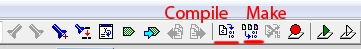
\includegraphics[scale=0.7]{Image/20.jpg}
\end{center}
\caption{Создание исполняемых файлов}
\end{figure}

Подключите отладочную плату STM32l-Discovery через разъем Mini USB к USB разъему компьютера. Для загрузки программы в микроконтроллер в главном меню выберите пункт 
\begin{center}
\textit{Project => Download and Debug}
\end{center}
или на панели инструментов \textit{Download and Debug} (Ctrl+D). 

 
\begin{figure}[h!]
\begin{center}
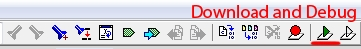
\includegraphics[scale=0.7]{Image/21.jpg}
\end{center}
\caption{Загрузка программы в микроконтроллер}
\end{figure}

После завершения загрузки программы в микроконтроллер, в IAR появиться панель отладки. 
\begin{figure}[h!]
\begin{center}
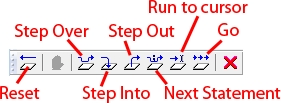
\includegraphics[scale=0.7]{Image/22.jpg}
\end{center}
\caption{Панель отладки}
\end{figure}

\textit{Step Over } -- выполняется следующая инструкция, оператор или функция, без входа в саму функцию.

\textit{Step Into } -- выполняется следующая инструкция, оператор или функция c входом в саму функцию.

\textit{Step Over } -- выполняется следующая инструкция, оператор или функция c выходом из функции.

\textit{Next Statement} -- выполняется следующая инструкция, оператор или функция без остановки вызовов функций.

\textit{Run to cursor} --  выполняется следующая инструкция, оператор или функция до выделенного фрагмента кода.

\textit{Reset} -- отладка выполняется с начала программы.

\textit{Go} -- выполняется следующая инструкция, оператор или функция до метки или окончания программы.

Для контроля значений переменных и функций используется инструмент \textit{Live Watch}. 
\begin{center}
\textit{View => Live Watch}
\end{center}
\textit{Live Watch} позволяет отслеживать значение выбранных переменных во время выполнения программы.
	Для запуска загруженной программы в микроконтроллер нажмите на панели отладки на \textit{Go} (F5).
	Все инструменты отладки дополнительно приведены в пункте \textit{Debug} в главном меню.





% \chapter{Работа №2. Работа с жидкокристаллическим индикатором}
Цель работы: 
\begin{itemize}
\item Изучение принципов работы ЖКИ.
\item Знакомство с регистрами контроллера ЖКИ, регистрами портов микроконтроллера.
\item Разработка программы для микроконтроллера без использования и с использованием SPL.
\end{itemize}

\section{Общие сведения}

На отладочной плате STM32L-Discovery установлен жидкокристаллический индикатор (ЖКИ, англ. LCD. Liquid crystal display), имеющий шесть 14 сегментных знаков, 4 знака двоеточия (Colon), 4 точки (DP), 4 полоски (Bar). Все сегменты объединены в группы СOM0, COM1, COM2, COM3 по 24 сегмента. Каждая группа имеет свой отдельный <<общий провод>>.

\begin{figure}[h!]
\begin{center}
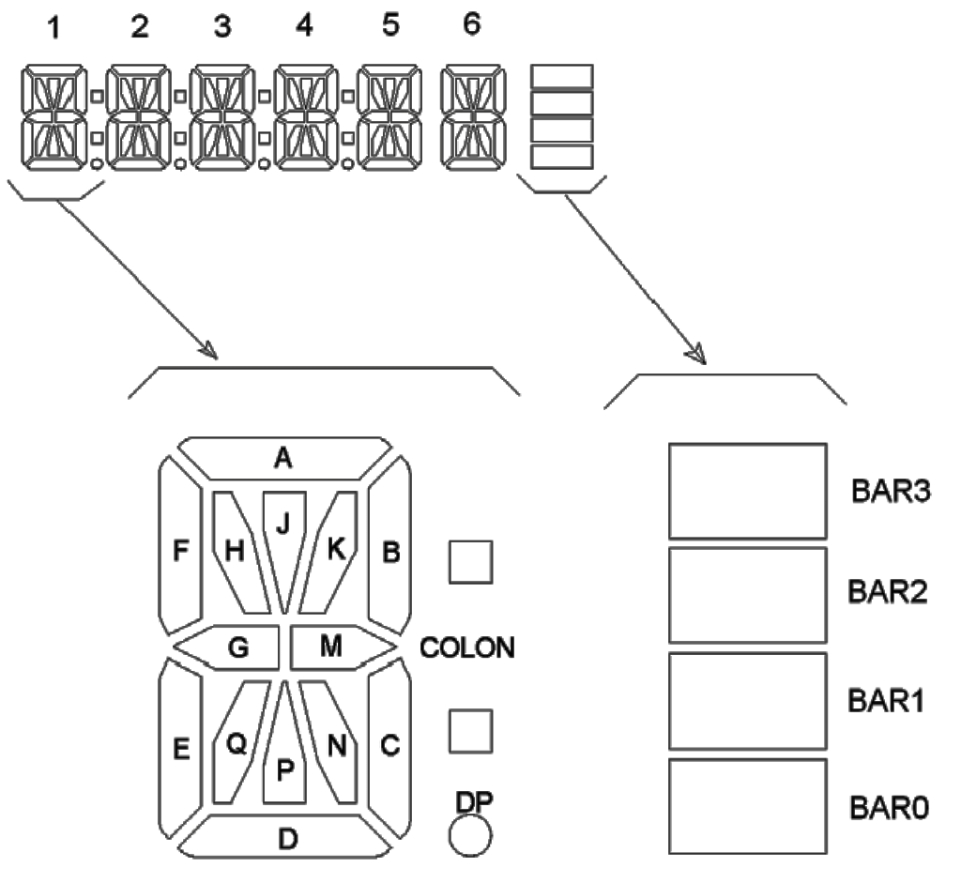
\includegraphics[scale=0.4]{Image/23.jpg}
\end{center}

\caption{Обозначение сегментов ЖКИ}
\end{figure}

\section{Контроллер ЖКИ}
\subsection{Основные функции}
В микроконтроллере есть встроенный контроллер ЖКИ \cite{datasheet}, который управляет монохромными жидкокристаллическими индикаторами. Контроллер ЖКИ:
\begin{enumerate}
\item Позволяет настраивать частоту обновлений (частоту кадров -- частота, с которой обновляется информация на ЖКИ)
\item Поддерживает статический и мультиплексный режим управления.
\item Поддерживает программную установку контраста.
\item Позволяет использовать несколько уровней управляющего напряжения (до четырех)
\item Использует двойную буферизацию, позволяющую обновлять данные в регистрах \textit{LCD\_RAM} в любое время выполнения программы, не нарушая целостность отображаемой информации.
\end{enumerate}

\begin{figure}[h!]
\begin{center}
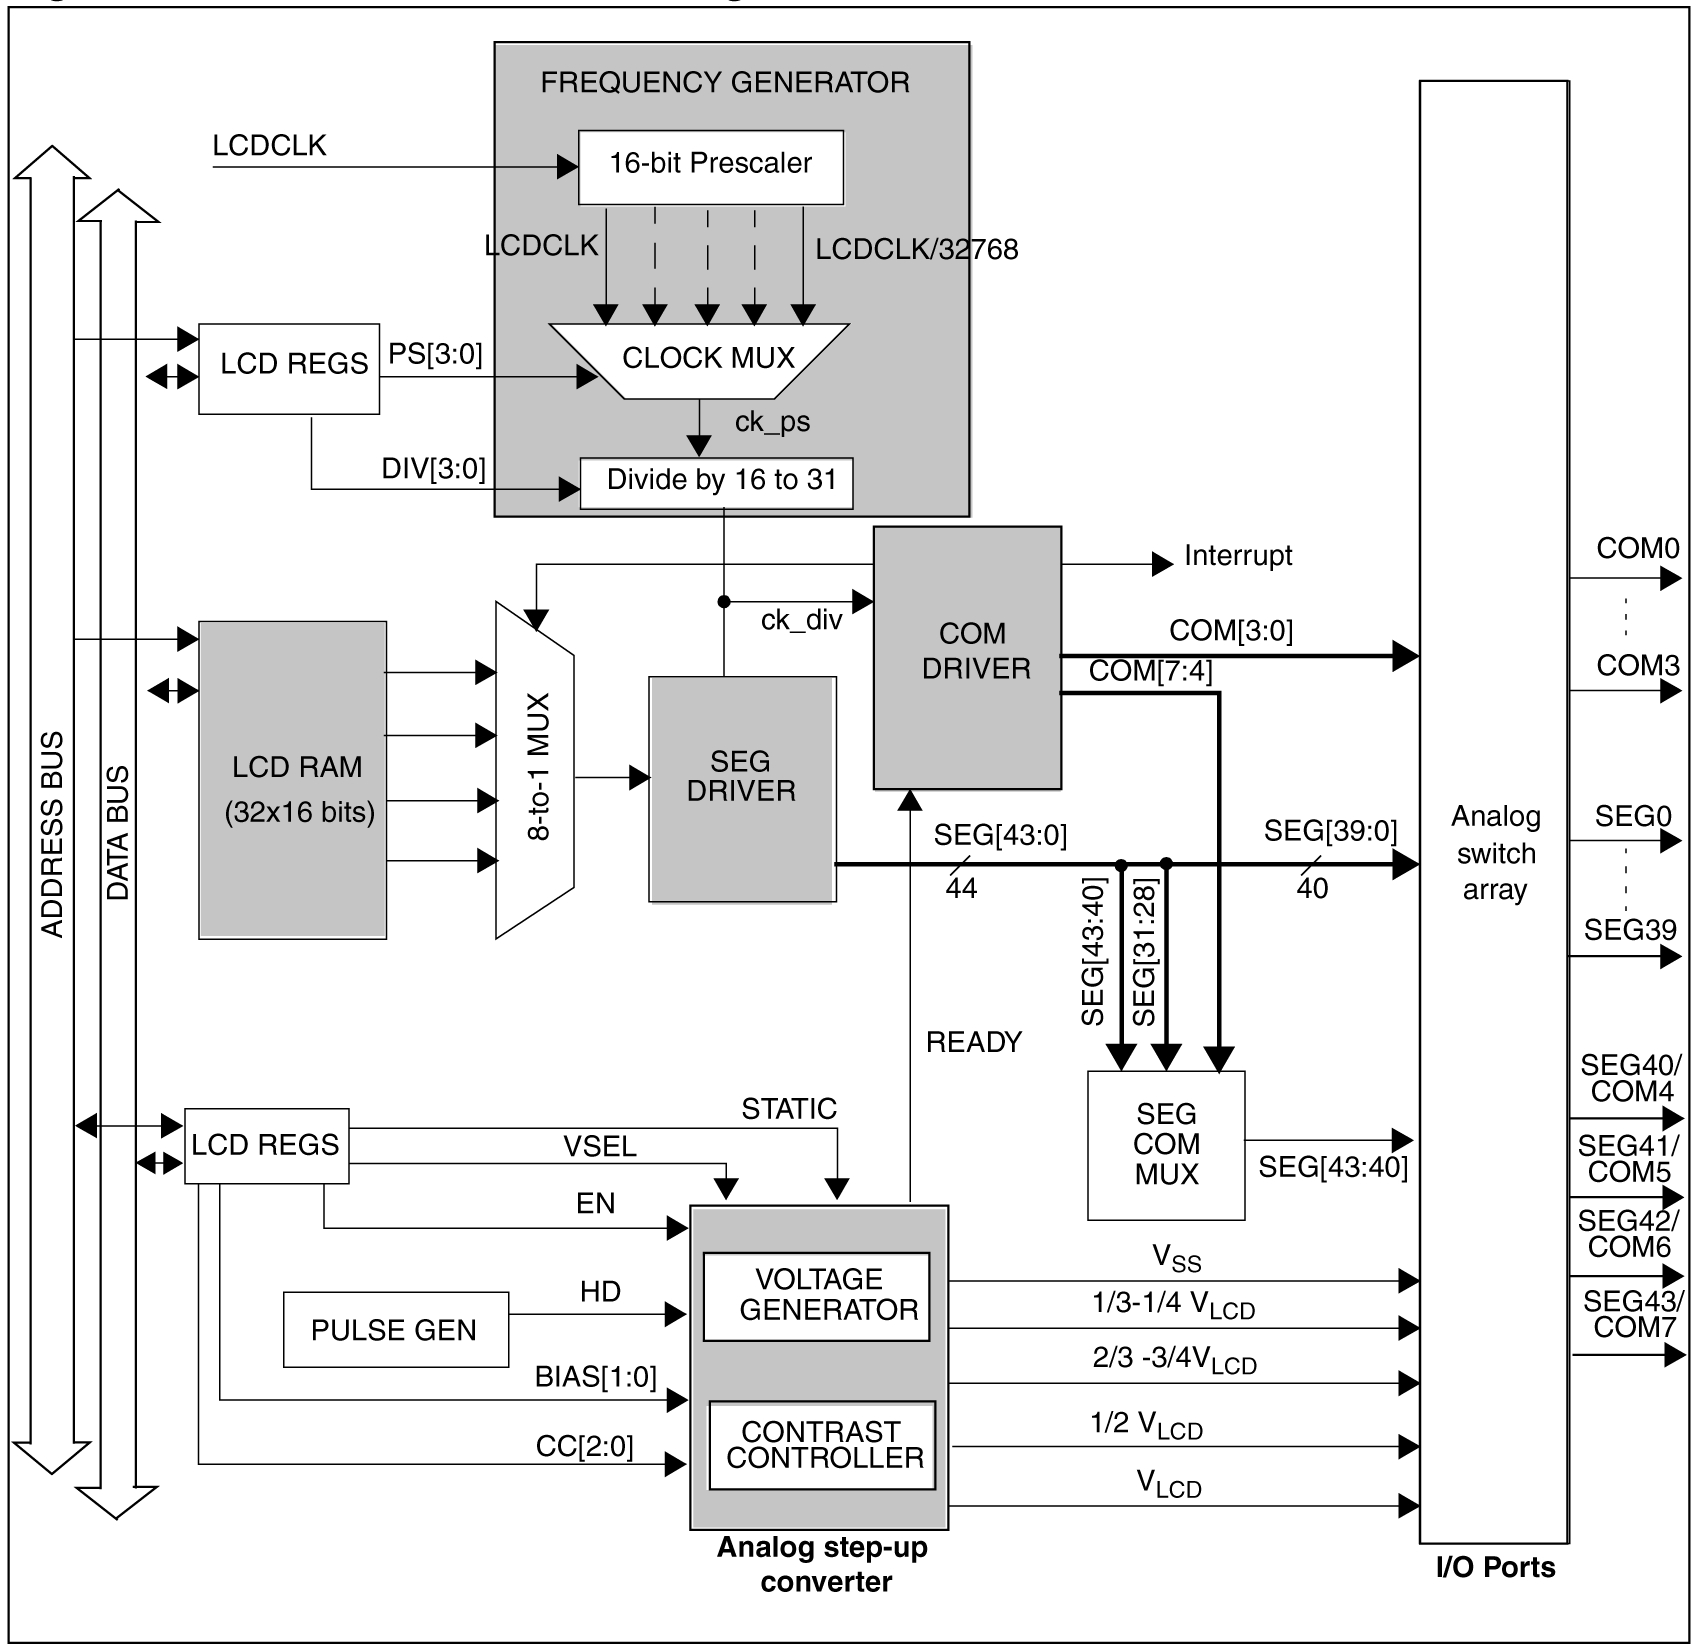
\includegraphics[scale=0.25]{Image/24.jpg}
\end{center}
\caption{Контроллер ЖКИ}
\end{figure}

\subsection{Регистры памяти контроллера ЖКИ}
\label{RegMemLCD}

В микроконтроллере STM32L152RB выделены специальные регистры \textit{LCD\_RAM} \cite{ReferManual}, информация, хранимая в которых, соответствует группе сегментов COM0 -- COM3. Каждой группе соответствует два 32 разрядных регистра. Такое количество регистров позволяет микроконтроллеру управлять ЖКИ c большим количеством сегментов, чем установленным на отладочной плате \cite{chip}.


\begin{figure}[h!]
\begin{center}
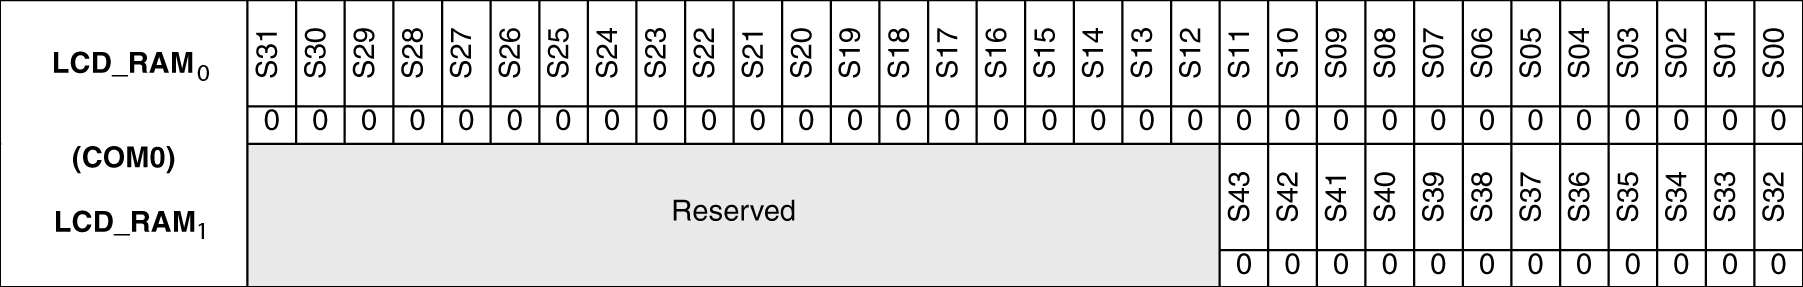
\includegraphics[scale=0.27]{Image/25.jpg}
\end{center}
\caption{Состав группы COM0}\label{COM0}
\end{figure}

Для управления ЖКИ со 176 сегментами используются 4 группы COM0 -- COM3 по 44 сегмента каждая, для управления ЖКИ с 320 сегментами используются 8 групп COM0 -- COM7 по 40 сегментов каждая.

\begin{figure}[h!]
\begin{center}
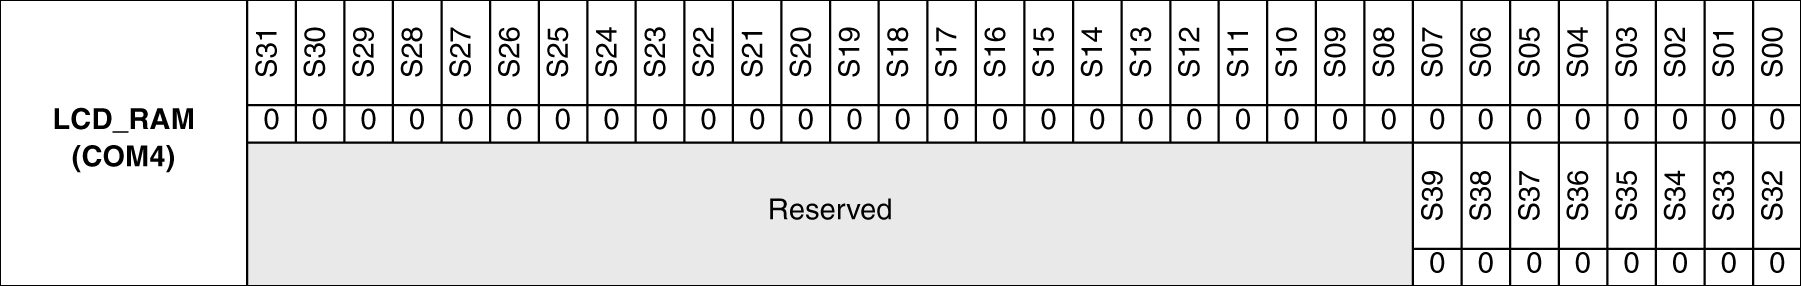
\includegraphics[scale=0.27]{Image/26.jpg}
\end{center}
\caption{Состав группы COM4}
\end{figure}

\begin{center}
\textit{В данной работе используется ЖКИ с 96 сегментами, разделенными на 4 группы COM0 -- COM3 по 24 сегмента каждая.}
\end{center}

\begin{figure}[h!]
\begin{center}
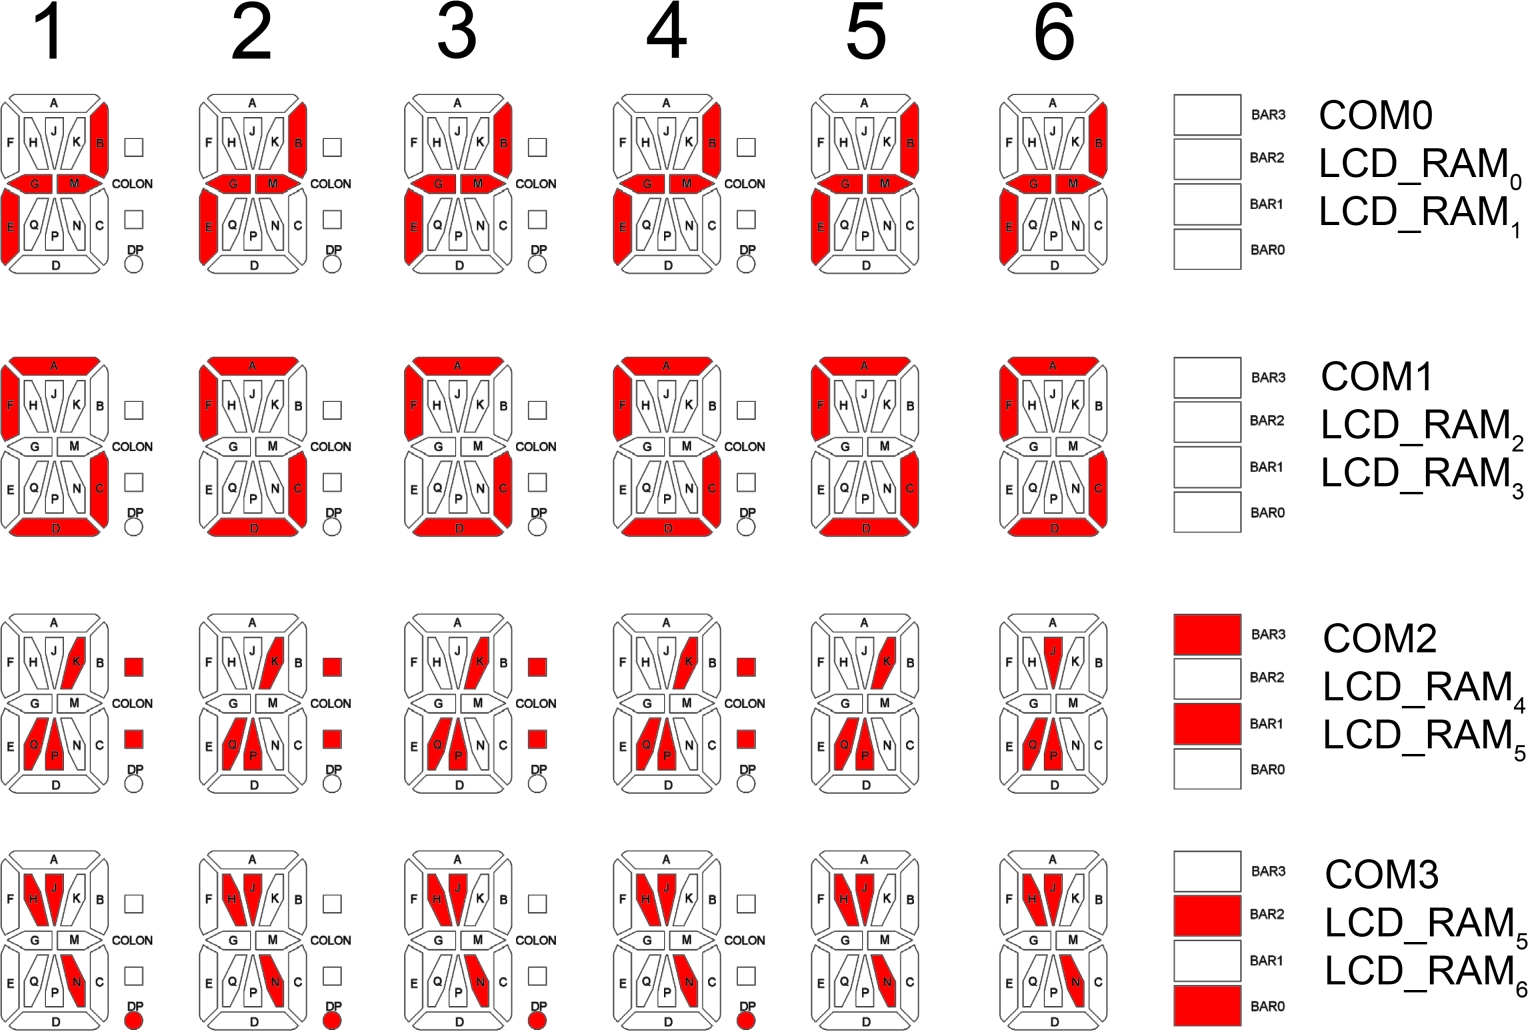
\includegraphics[scale=0.33]{Image/27.jpg}
\end{center}
\caption{Объединение сегментов в группы}\label{segment}
\end{figure}

ЖКИ на отладочной плате STM32L-Discovery подключен таким образом, что используются биты  \textit{S40, S41} вторых регистров \textit{LCD\_RAM} в каждой группе и биты  \textit{S0 -- S27} первых регистров \textit{LCD\_RAM}. Для уменьшения количества используемых регистров, информацию из битов  \textit{S40 --S43 }можно записывать в свободные биты  \textit{S28 -- S31}, используя \textit{функцию переназначения (remapping)}. 

\subsection{Блок делителей частоты}

Блок делителей частоты (Frequency generator) позволяет добиться различной частоты кадров (frame rates) на ЖКИ в диапазоне от 32 кГц до 1 МГц. В качестве источника тактирующего сигнала могут использоваться:
\begin{enumerate}
\item Внешний НЧ генератор с частотой 32 кГц (LSE. Low speed external).
\item Внутренний НЧ генератор с частотой 37 кГц (LSI. Low speed internal).
\item Внешний ВЧ генератор с делителями частоты на 2,4,8 и 16 и максимальной частотой 1 МГц. (HSE. High speed external)
\end{enumerate}

Для достижения точной синхронизации и снижения смещения напряжения постоянного тока через сегменты ЖКИ источник тактирующего сигнала должен обладать стабильностью. 

Тактирующий сигнал \textit{LCDCLK} поступает в контроллер ЖКИ. Частота тактового сигнала делится, в соответствии с коэффициентами деления, которые устанавливаются битами \textit{PS[3:0]}, \textit{DIV[3:0]} регистра \textit{LCD\_FCR }(Frame Control Register). Результирующая частота на выходе блока делителей частоты рассчитывается по формуле:


\[f_{ck\_div}=\frac{F_{LCDCLK}}{2^{PS}\cdot(16+DIV)}\]
Частота кадров рассчитывается по формуле:

\[ f_{Frame}=f_{ck\_div}\cdot duty\]
где $duty$ --- коэффициент заполнения -- отношение длительность импульса к его периоду. 

За время одного кадра на ЖКИ последовательно выводится информация из регистров \textit{LCD\_RAM[x]}, \textit{LCD\_RAM[x+1]} и тд. Для ЖКИ, установленного на отладочной плате, за один кадр, контроллер ЖКИ должен вывести информацию из 4 групп сегментов \textit{COM0 -- COM3}, следовательно, длительность управляющего импульса для одной группы будет 1/4 длительности кадра, т.е. \textit{duty=1/4}. 

\section{Динамическая и статическая индикация. Управление ЖКИ}

Существует два способа управления ЖКИ -- \textit{статический} режим управления и \textit{мультиплексный}\cite{gost25} режим управления. При статической индикации каждый сегмент разряда индикатора подключен к выходу микроконтроллера. Применительно к ЖКИ на отладочной плате STM32L-Discovery потребуется 6*14 = 84 выводов микроконтроллера (без учета двоеточий, точек и полосок). Из-за использования такого количества выводов, подключение другой периферии станет невозможным. Микроконтроллер STM32L152RB имеет 64 вывода.
	
	При мультиплексном режиме управлении (динамический режим управления) одинаковые сегменты разрядов индикатора объединены в группы. Отображение информации происходит за счет поочередного зажигания сегментов разрядов индикатора, с частотой, не воспринимаемой человеческим глазом. На рисунке \ref{t0} -- \ref{t3} условно изображен принцип работы динамической индикации. На ЖКИ выводится число 3114.


\begin{figure}[H]
\begin{center}
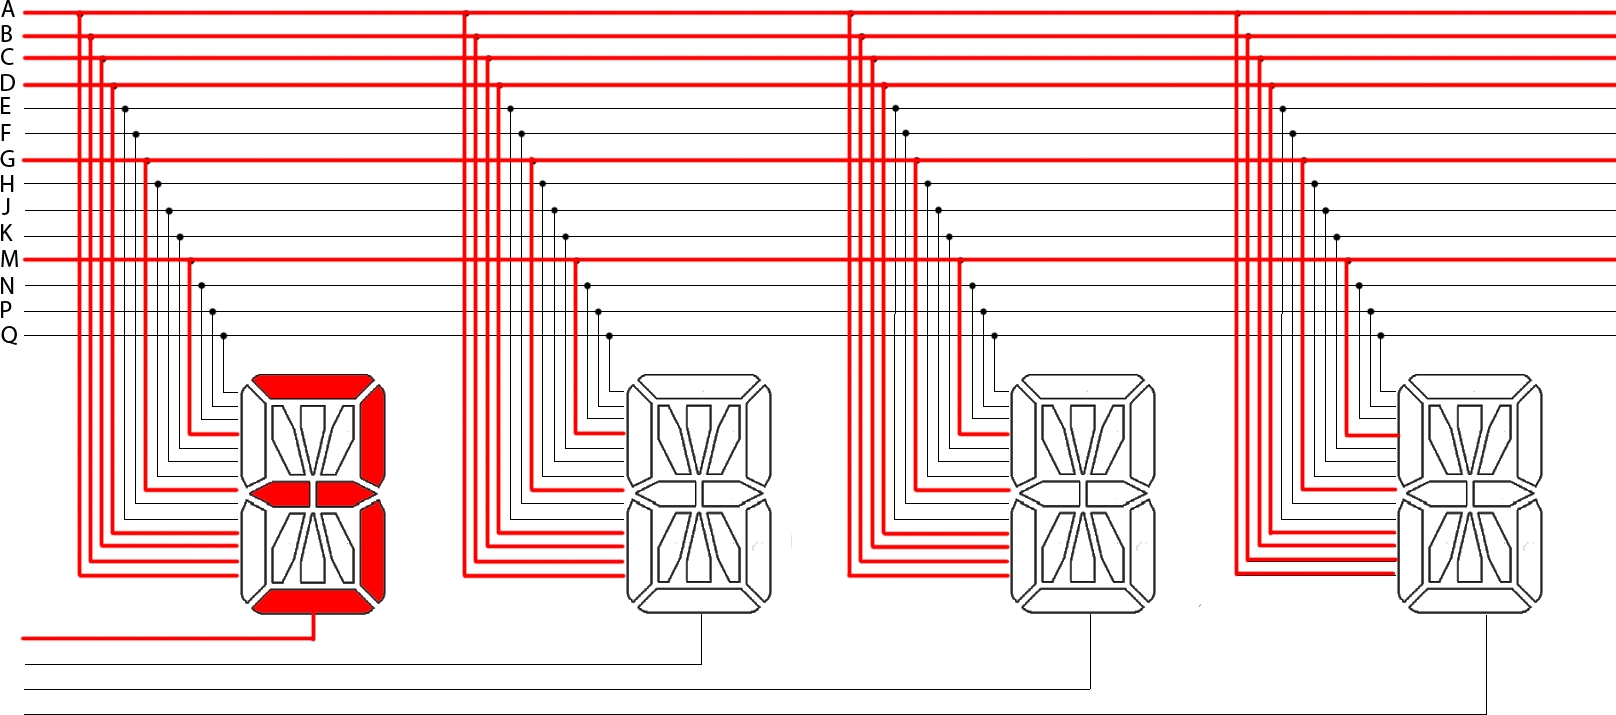
\includegraphics[scale=0.28]{Image/28.jpg} 
\end{center}
\caption{Работа ЖКИ в момент времени $t_0$}\label{t0}
\end{figure}

\begin{figure}[H]
\begin{center}
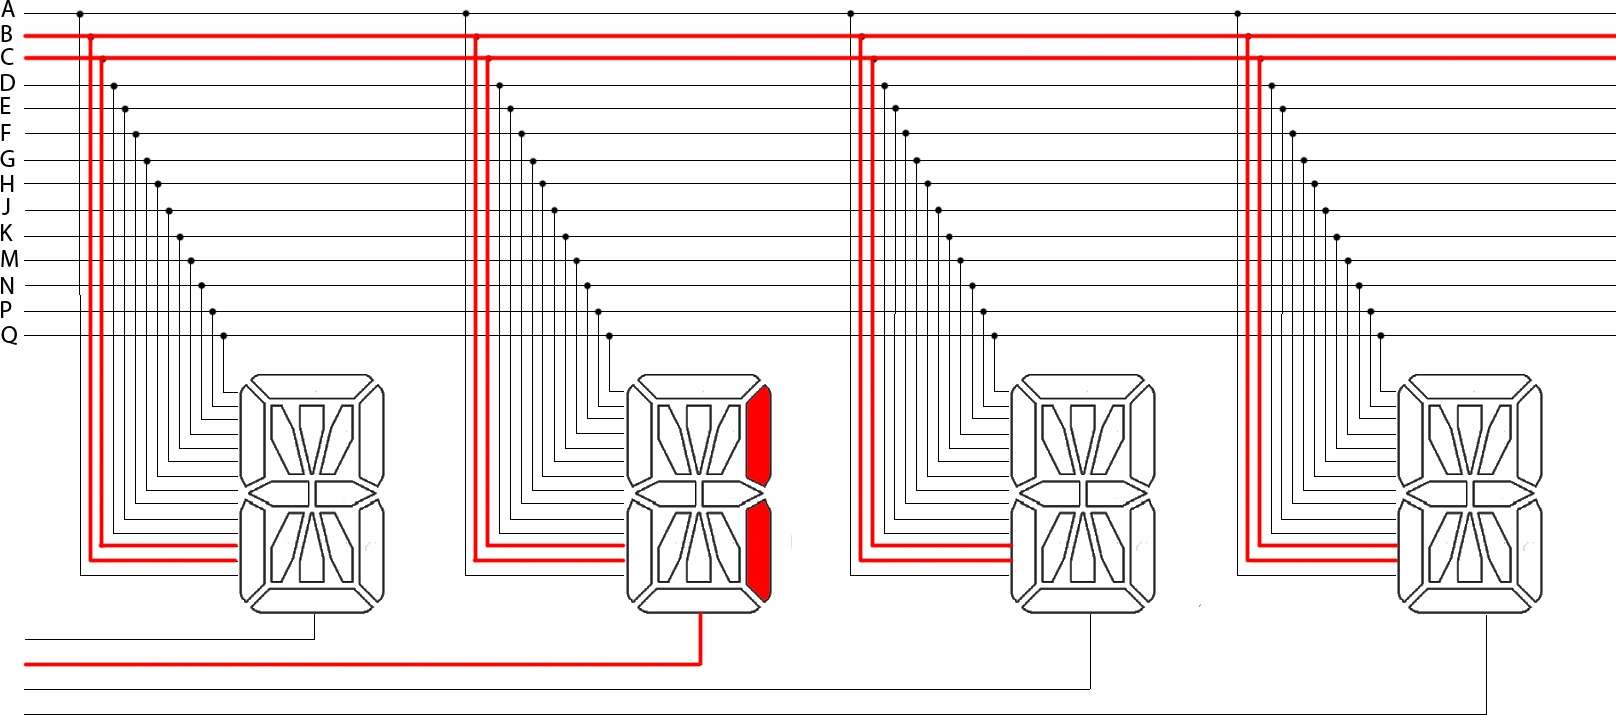
\includegraphics[scale=0.28]{Image/29.jpg}
\end{center}
\caption{Работа ЖКИ в момент времени $t_1$}
\end{figure}


\begin{figure}[H]
\begin{center}
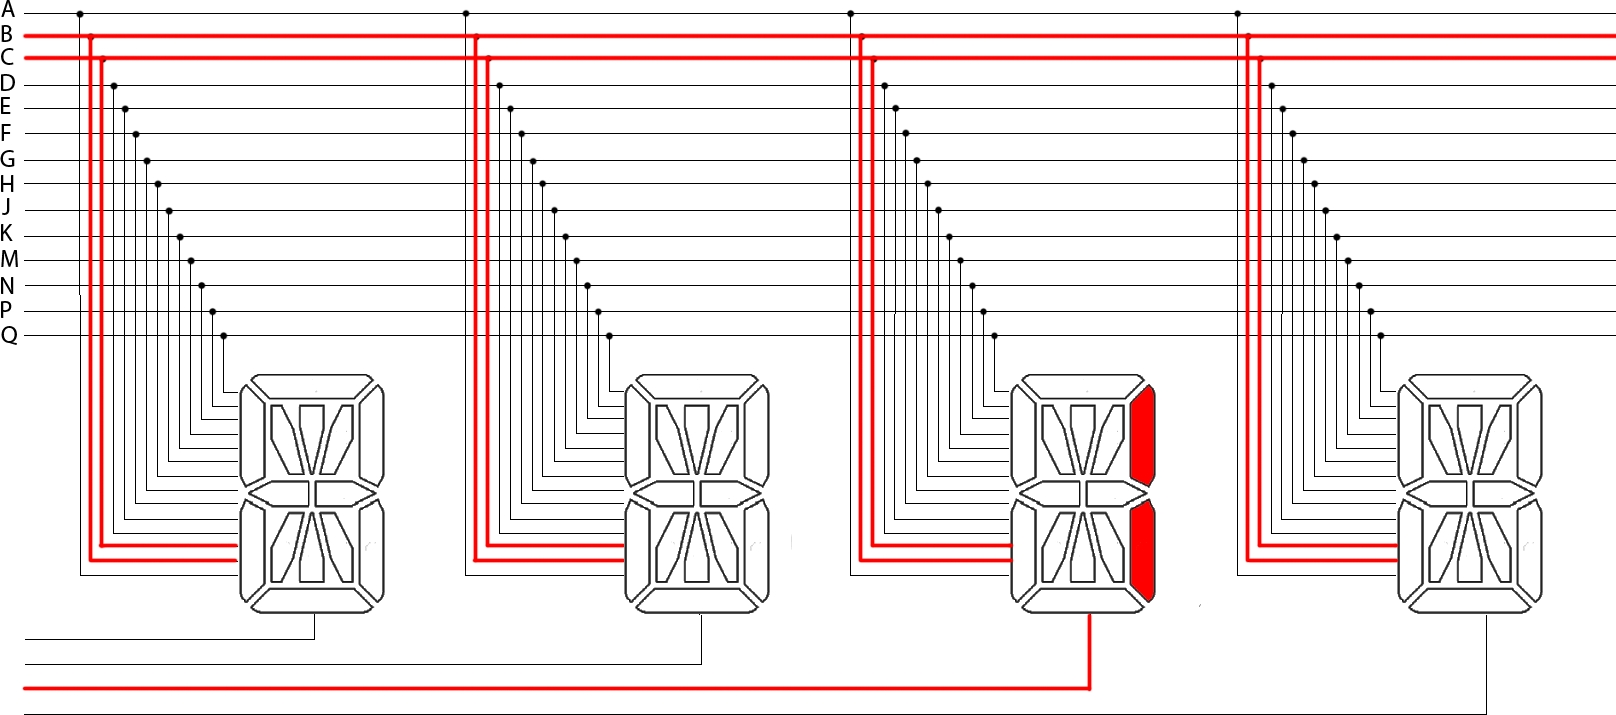
\includegraphics[scale=0.28]{Image/30.jpg}
\end{center}
\caption{Работа ЖКИ в момент времени $t_2$}
\end{figure}

\begin{figure}[H]
\begin{center}
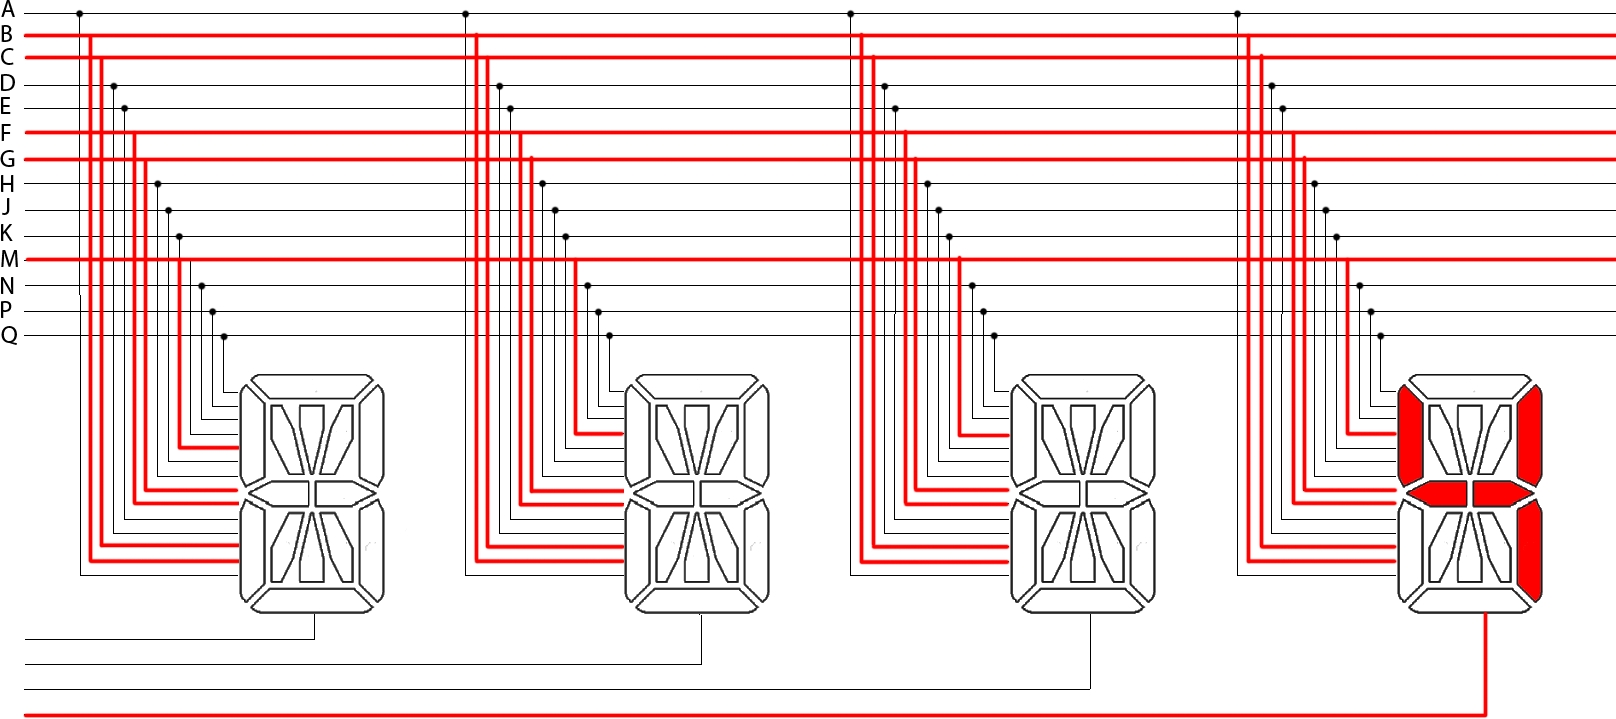
\includegraphics[scale=0.28]{Image/31.jpg} 
\end{center}
\caption{Работа ЖКИ в момент времени $t_3$}\label{t3}
\end{figure}

Мультиплексное управление позволяет управлять большим количеством сегментов. Вместо раздельного управления каждым элементом, они могу адресоваться по строкам и столбцам (COM и SEG (обозначение сегментов приведено на рисунке \ref{shema})), таким образом, упрощается управляющая схема, т.к. каждому сегменту не требуется собственная управляющая линия. Для включения выбранного сегмента, на него надо подать разность потенциалов \textit{COM} и \textit{SEG}. Пример работы первого разряда индикатора, используемого в данной работе, изображен на рисунке \ref{t01} -- \ref{t31}. На индикатор выводится <<1:>>.

\begin{figure}[H]
\begin{center}
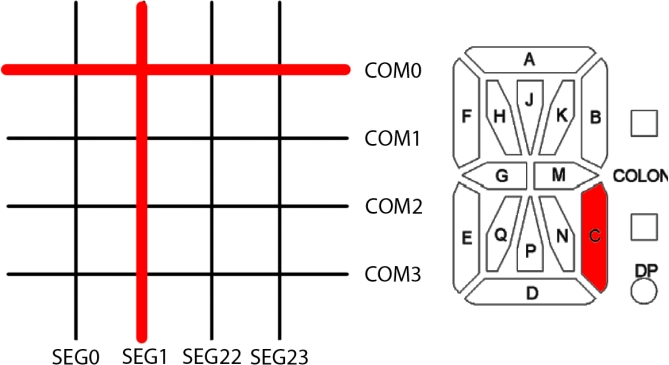
\includegraphics[scale=0.4]{Image/32.jpg} 
\end{center}
\caption{Первый разряд индикатора в момент времени $t_0$}\label{t01}
\end{figure}


\begin{figure}[H]
\begin{center}
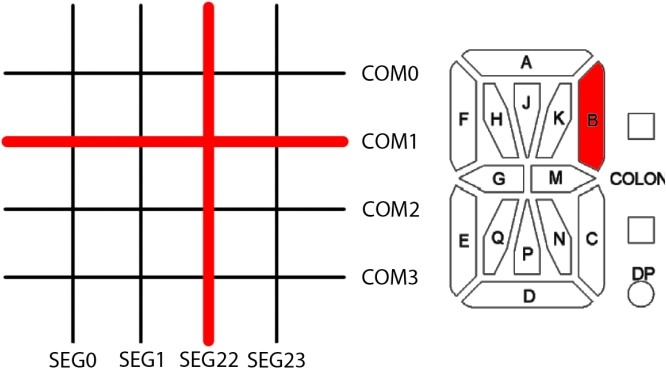
\includegraphics[scale=0.4]{Image/33.jpg} 
\end{center}
\caption{Первый разряд индикатора в момент времени $t_1$}
\end{figure}


\begin{figure}[H]
\begin{center}
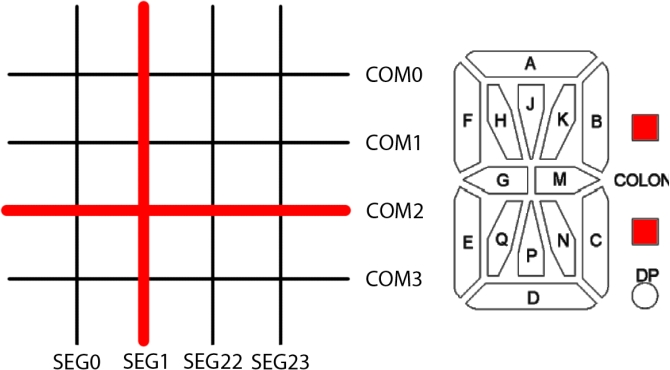
\includegraphics[scale=0.4]{Image/34.jpg} 
\end{center}
\caption{Первый разряд индикатора в момент времени $t_2$}\label{t31}
\end{figure}

Общая схема подключения сегментов к выводам ЖКИ \cite{scheme} приведена на рисунке \ref{shema}.


\begin{figure}[H]
\begin{center}
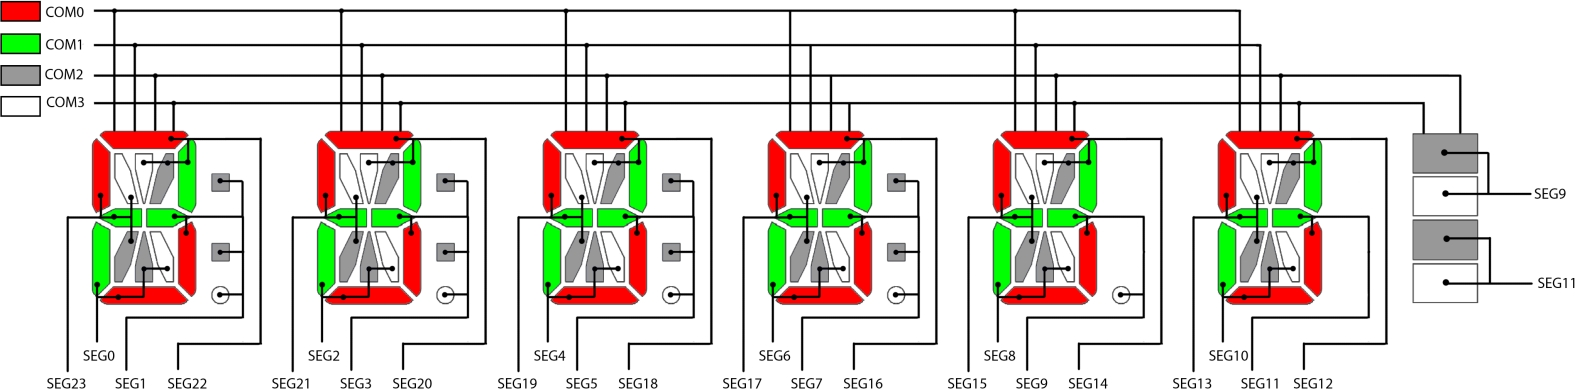
\includegraphics[scale=0.33]{Image/35.jpg} 
\end{center}
\caption{Схема подключения сегментов к выводам ЖКИ}\label{shema}
\end{figure}

Схема подключения выводов ЖКИ к портам микроконтроллера приведена на рисунке \ref{shema2}.


\begin{figure}[H]
\begin{center}
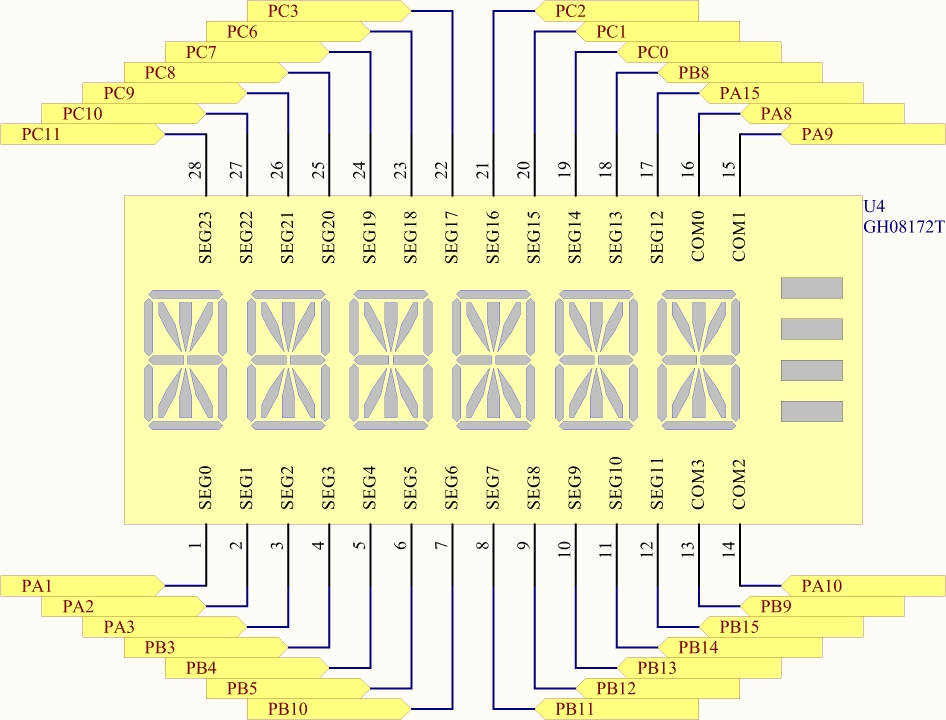
\includegraphics[scale=0.38]{Image/36.jpg} 
\end{center}
\caption{Схема подключения выводов ЖКИ к портам микроконтроллера}\label{shema2}
\end{figure}

Для линий \textit{SEG} используется управляющее напряжение, количество уровней которого определяется коэффициентом \textit{bias}. ЖКИ на отладочной плате использует мультиплексный режим управления с \textit{duty=1/4} и\textit{ bias=1/3}. Значение duty и bias устанавливаются через регистр \textit{LCD\_CR} (Control Register) в битах \textit{DUTY[2:0]} и\textit{ BIAS[1:0]}. Форма управляющих напряжений для \textit{duty=1/4} и \textit{bias=1/3} приведена на рисунке \ref{pit}.

\begin{figure}[H]
\begin{center}
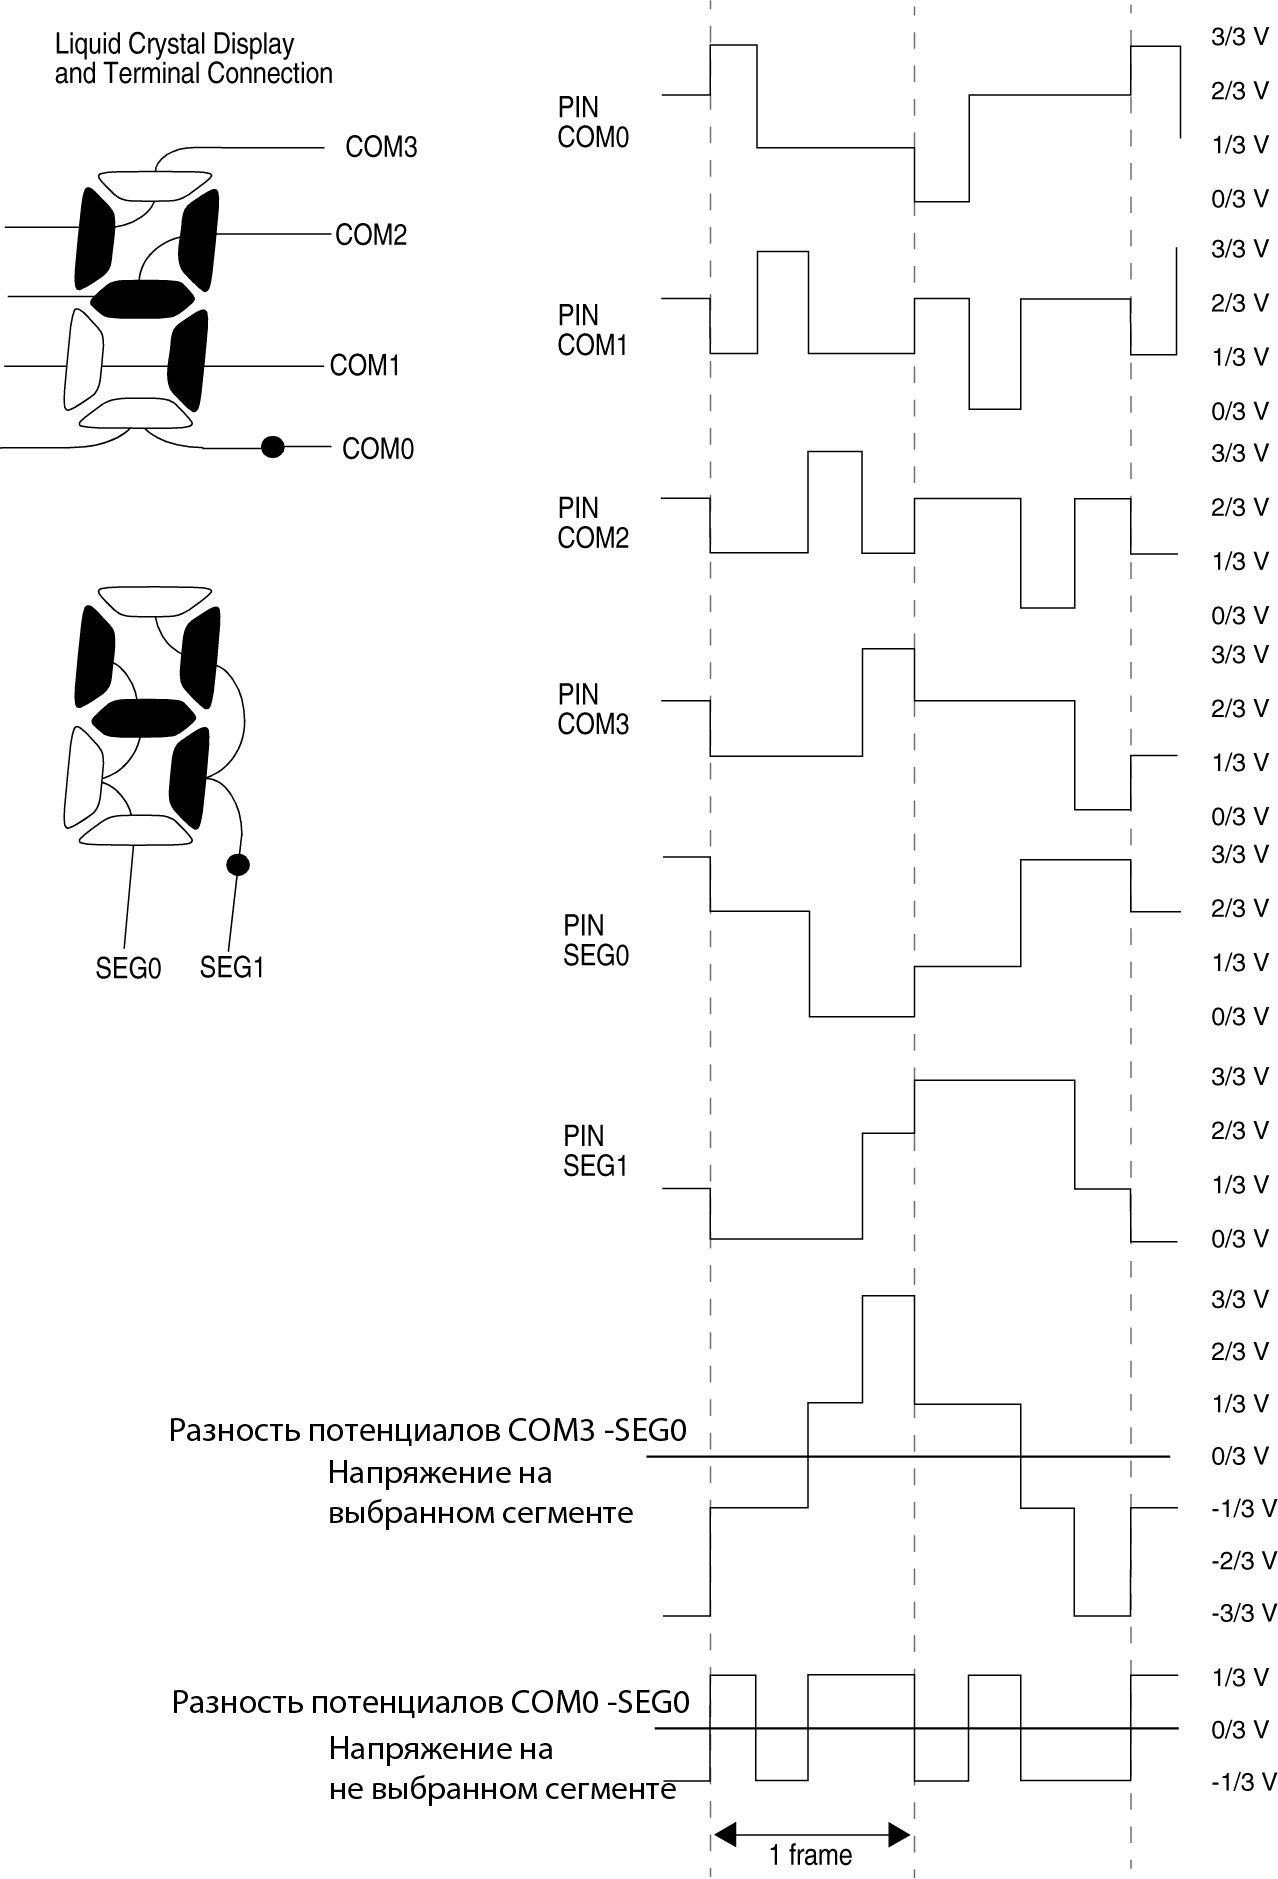
\includegraphics[scale=0.33]{Image/37.jpg} 
\end{center}
\caption{Форма управляющих сигналов}\label{pit}
\end{figure}

\section{Конфигурирование микроконтроллера}
\subsection{Регистры периферии. Запись в регистры}

Для управления ЖКИ порты микроконтроллера должны быть настроены соответствующим образом:
\begin{enumerate}
\item На выход.
\item Использование альтернативной функции \textit{AF 11} (Alternate function).
\item Иметь частоты вывода в порт 400 кГц.
\item Использовать режим работы \textit{push -- pull}.
\item Без подтягивающих резисторов. 
\end{enumerate}


При работе порта в режиме альтернативной функции, выходной буфер данных порта управляется сигналами, поступающими с периферии. Заголовочный файл \textit{stm32l1xx.h} библиотеки CMSIS содержит описание всех регистров периферии, объединенных в структуры:
\begin{verbatim}
...
typedef struct
{
  __IO uint32_t MODER;
  __IO uint16_t OTYPER;
  uint16_t RESERVED0;
  __IO uint32_t OSPEEDR;
  __IO uint32_t PUPDR;
  __IO uint16_t IDR;
  uint16_t RESERVED1;
  __IO uint16_t ODR;
  uint16_t RESERVED2;
  __IO uint16_t BSRRL; /* BSRR register is split to 
                    		  2 * 16-bit fields BSRRL 
  __IO uint16_t BSRRH; /* BSRR register is split to 
                       2 * 16-bit fields BSRRH 
  __IO uint32_t LCKR;
  __IO uint32_t AFR[2];
} GPIO_TypeDef;
...
typedef struct
{
  __IO uint32_t CR;
  __IO uint32_t ICSCR;
  __IO uint32_t CFGR;
  __IO uint32_t CIR;
  __IO uint32_t AHBRSTR;
  __IO uint32_t APB2RSTR;
  __IO uint32_t APB1RSTR;
  __IO uint32_t AHBENR;
  __IO uint32_t APB2ENR;
  __IO uint32_t APB1ENR;
  __IO uint32_t AHBLPENR;
  __IO uint32_t APB2LPENR;
  __IO uint32_t APB1LPENR;      
  __IO uint32_t CSR;    
} RCC_TypeDef;
...
\end{verbatim}
Для удобного обращения определены константы:
\begin{verbatim}
...
#define RCC                 ((RCC_TypeDef *) RCC_BASE)
#define CRC                 ((CRC_TypeDef *) CRC_BASE)
...
#define GPIOA               ((GPIO_TypeDef *) GPIOA_BASE)
#define GPIOB               ((GPIO_TypeDef *) GPIOB_BASE)
#define GPIOC               ((GPIO_TypeDef *) GPIOC_BASE)
#define GPIOD               ((GPIO_TypeDef *) GPIOD_BASE)
#define GPIOE               ((GPIO_TypeDef *) GPIOE_BASE)
#define GPIOH               ((GPIO_TypeDef *) GPIOH_BASE)
...

\end{verbatim}

Определенные таким образом структуры и указатели используются для доступа к конкретным регистрам периферии. Пример записи значения в регистр \textit{MODER} порта \textit{GPIOA}:
\begin{verbatim}
GPIOA->MODER = 0x4;
\end{verbatim}
Пример записи значения в регистр \textit{AHBENR }системы тактирования и сброса \textit{RCC}:

\begin{verbatim}
RCC->AHBENR = 0x7;
\end{verbatim}
Для упрощения записи значений в регистры, в файле \verb\stm32lxx.h\, заранее определены битмаски --- расшифровка отдельных битов регистров по функциям. Вместо использования шестнадцатеричных значений используются заранее определенные константы.

\begin{verbatim}
...
#define GPIO_MODER_MODER1          ((uint32_t)0x0000000C)
#define GPIO_MODER_MODER1_0        ((uint32_t)0x00000004)
#define GPIO_MODER_MODER1_1        ((uint32_t)0x00000008)
#define GPIO_MODER_MODER2          ((uint32_t)0x00000030)
...
\end{verbatim}
Пример записи значения в регистр \textit{MODER} порта \textit{GPIOA}:
\begin{verbatim}
GPIOA->MODER |= GPIO_MODER_MODER1_0;
\end{verbatim}
Результат выполнения строки аналогичен \verb#GPIOA->MODER = 0x4#;

%%%%%%%%%%%%%%%%%%%%%%%%%%%%%%%%%%%%%%%%%%%%


%Дописать


%%%%%%%%%%%%%%%%%%%%%%%%%%%%%%%%%%%%%%%%%%%
\subsection{Конфигурирование портов микроконтроллера}

Выводы ЖКИ подключены к портам \textit{GPIOA} (PA1 -- PA3, PA8 -- PA10, PA15), \textit{GPIOB} (PB3 -- PB5, PB8 -- PB15), \textit{GPIOC} (PC0 -- PC3, PC6 -- PC11) микроконтроллера. (см. рисунок \ref{shema2}). Для работы ЖКИ на выбранные порты необходимо подать тактовый сигнал. Тактирование портов\textit{ GPIO} микроконтроллера происходит от шины \textit{AHB} системы \textit{RCC} (Reset and Clock Control) -- системы тактировании и сброса. Подача тактового сигнала осуществляется установкой соответствующих битов в регистре \textit{RCC\_AHBENR} (AHB peripheral clock enable register). 


\begin{figure}[H]
\begin{center}
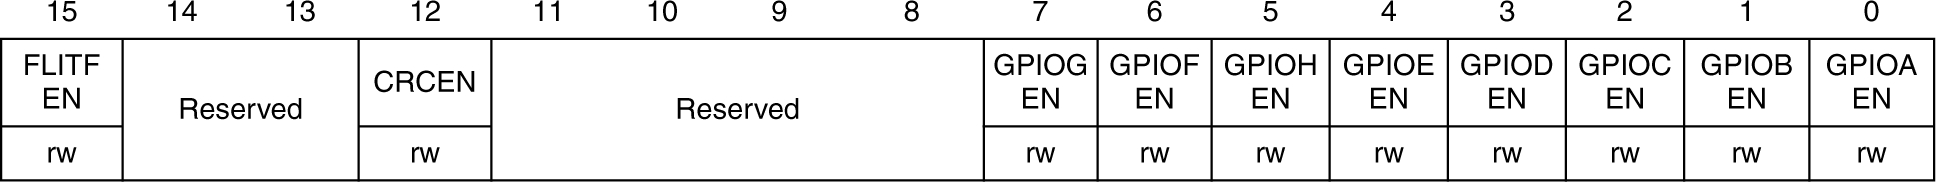
\includegraphics[scale=0.25]{Image/38.jpg} 
\end{center}
\caption{Регистр \textit{RCC\_AHBENR} (приведены первые 15 разрядов)}
\end{figure}

Для портов \textit{GPIOA, GPIOB, GPIOC} необходимо установить \verb\1\ в 0, 1, 2 разряды регистра. 

\begin{verbatim}
RCC->AHBENR |= (RCC_AHBENR_GPIOAEN | RCC_AHBENR_GPIOBEN
                | RCC_AHBENR_GPIOCEN)
                
// RCC->AHBENR = 0x7; 
// 0x7 = 111
\end{verbatim}

	Для указания режимов работы порта используется регистр \textit{GPIOx\_MODER} (GPIO port mode register) (x = A \ldots H). Все разряды регистра сгруппированы в группы \textit{MODERy[1:0]}, где y номер пина соответствующего порта. Порты необходимо настроить на режим альтернативной функции, т.е. в группе, отвечающей за пин, установить значение \verb\10\. Для порта \textit{GPIOA }нужно настроить пины 1 -- 3, 8 -- 10, 15, т.е установить \verb\1\ в 3, 5, 7, 17, 19, 21, 31 разряды. 


\begin{figure}[H]
\begin{center}
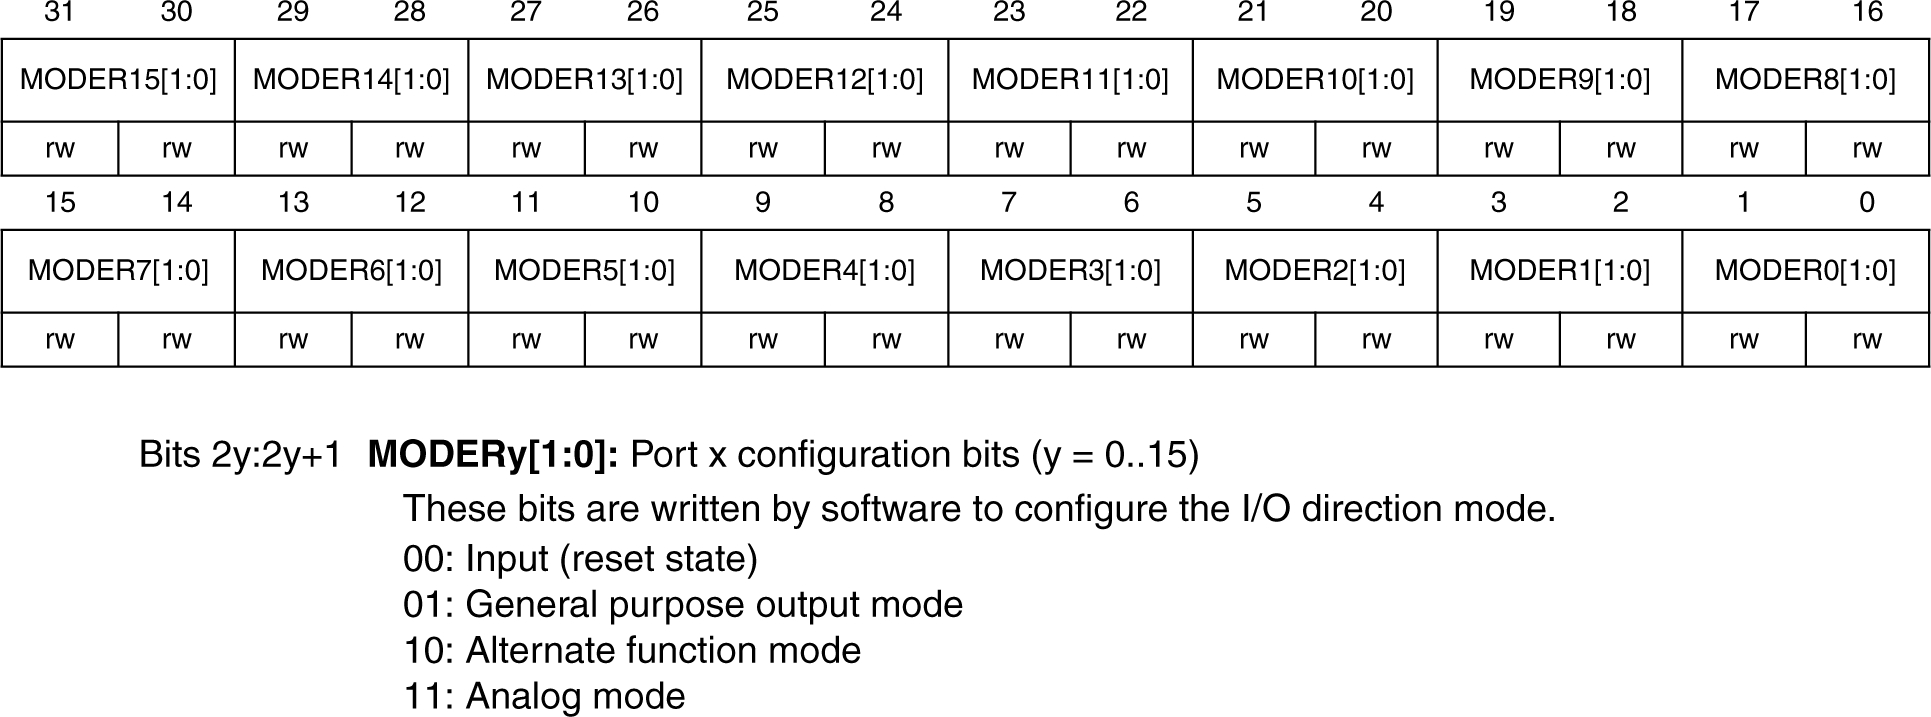
\includegraphics[scale=0.25]{Image/39.jpg} 
\end{center}
\caption{Регистр \textit{GPIOx\_MODER} (GPIO port mode register)}
\end{figure}
\begin{verbatim}
GPIOA->MODER |= (GPIO_MODER_MODER1_1 | GPIO_MODER_MODER2_1 
               | GPIO_MODER_MODER3_1 | GPIO_MODER_MODER8_1 |
                 GPIO_MODER_MODER9_1 | GPIO_MODER_MODER10_1 | 
                 GPIO_MODER_MODER15_1);

// GPIOA->MODER = 0x802A00A8;
// 0x802A00A8 = 1000 0000 0010 1010 0000 0000 1010 1000 
\end{verbatim}


Порты микроконтроллера необходимо перевести в режим \textit{push -- pull}. Для этого необходимо в регистре \textit{GPIOx\_OTYPER} (GPIO port output type register) установить \verb\1\ в разряды, отвечающие за пины. 
\begin{figure}[H]
\begin{center}
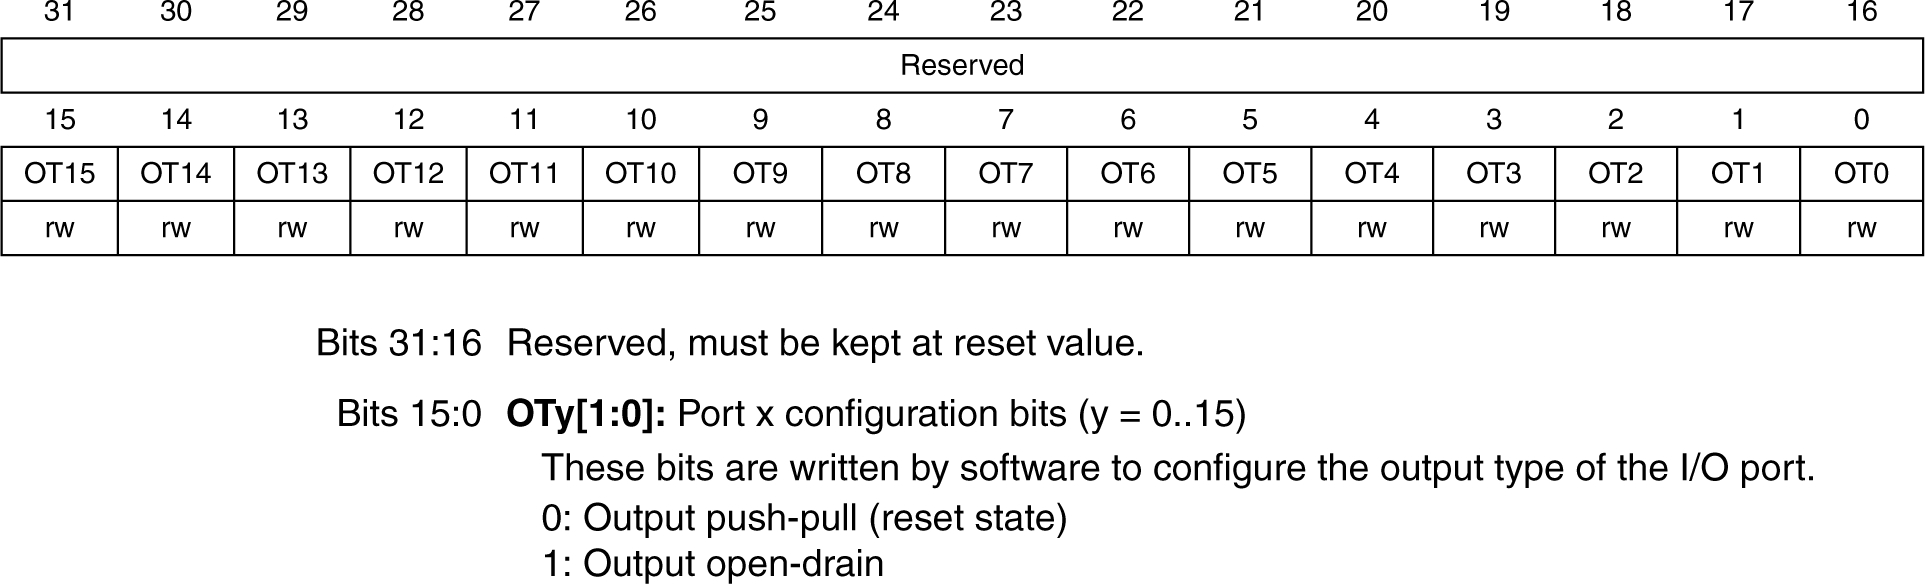
\includegraphics[scale=0.25]{Image/40.jpg} 
\end{center}
\caption{Регистр \textit{GPIOx\_OTYPER} (GPIO port output type register)}
\end{figure}

\begin{verbatim}
GPIOA->OTYPER &= ~(GPIO_OTYPER_OT_1 | GPIO_OTYPER_OT_2 |
                   GPIO_OTYPER_OT_3 | GPIO_OTYPER_OT_8 | 
                   GPIO_OTYPER_OT_9 | GPIO_OTYPER_OT_10 |
                   GPIO_OTYPER_OT_15);

// GPIOA->OTYPER &= ~0x0000870E;
// 0x870E = 1000 0111 0000 1110 
\end{verbatim}

Оба варианта воздействуют на выбранные пины. (Для порта GPIOA настраиваются пины 1 -- 3, 8 -- 10, 15). Если необходимо перевести все пины порта в режим \textit{push -- pull}, можно записать в регистр значение:

\begin{verbatim}
GPIOA->OTYPER = 0x0;
\end{verbatim}


Для указания частоты вывода информации в порт используется регистр \textit{ GPIOx\_OSPEEDR} (GPIO port output speed register). Все разряды регистра сгруппированы в группы \textit{OSPEEDRy[1:0]}, где y номер пина соответствующего порта. В данной работе должна быть установлена частота 400 кГц т.е. в группе, отвечающей за пин, установить значение \verb\00\. 


\begin{figure}[H]
\begin{center}
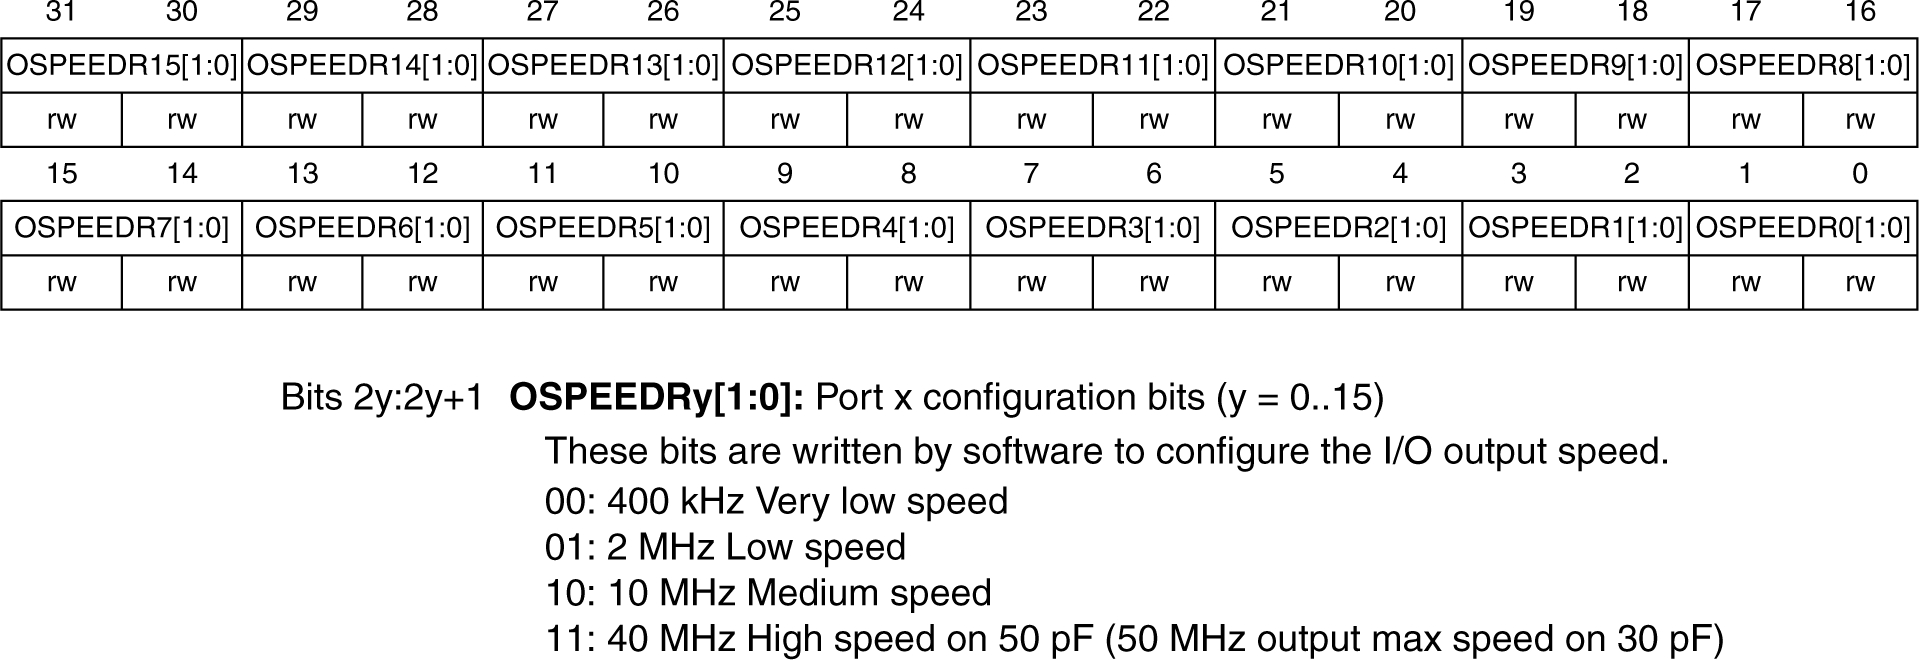
\includegraphics[scale=0.25]{Image/41.jpg} 
\end{center}
\caption{Регистр \textit{ GPIOx\_OSPEEDR} (GPIO port output speed register)}
\end{figure}

\begin{verbatim}
GPIOA->OSPEEDR &= ~(GPIO_OSPEEDER_OSPEEDR1 | GPIO_OSPEEDER_OSPEEDR2 |
                    GPIO_OSPEEDER_OSPEEDR3 | GPIO_OSPEEDER_OSPEEDR8 | 
                    GPIO_OSPEEDER_OSPEEDR9 | GPIO_OSPEEDER_OSPEEDR10 | 
                    GPIO_OSPEEDER_OSPEEDR15);

// GPIOA->OSPEEDR &= ~0xC03F00FC;
// 0xC03F00FC = 1100 0000 0011 1111 0000 0000 1111 1100 
\end{verbatim}
Если необходимо установить частоту вывода в порт 400 кГц для всех пинов, можно записать в регистр значение:
\begin{verbatim}
GPIOA->OSPEEDR = 0x0;
\end{verbatim}

Для отключения подтягивающих резисторов \textit{pull-up, pull-down} для выбранных пинов используется регистр \textit{GPIOx\_PUPDR }(GPIO port pull-up/pull-down register). Все разряды регистра сгруппированы в группы \textit{PUPDRy[1:0]}, где \textit{y} -- номер пина соответствующего порта. Для отключение подтягивающих резисторов в группе, отвечающей за пин, устанавливается значение \verb\00\. 

\begin{figure}[H]
\begin{center}
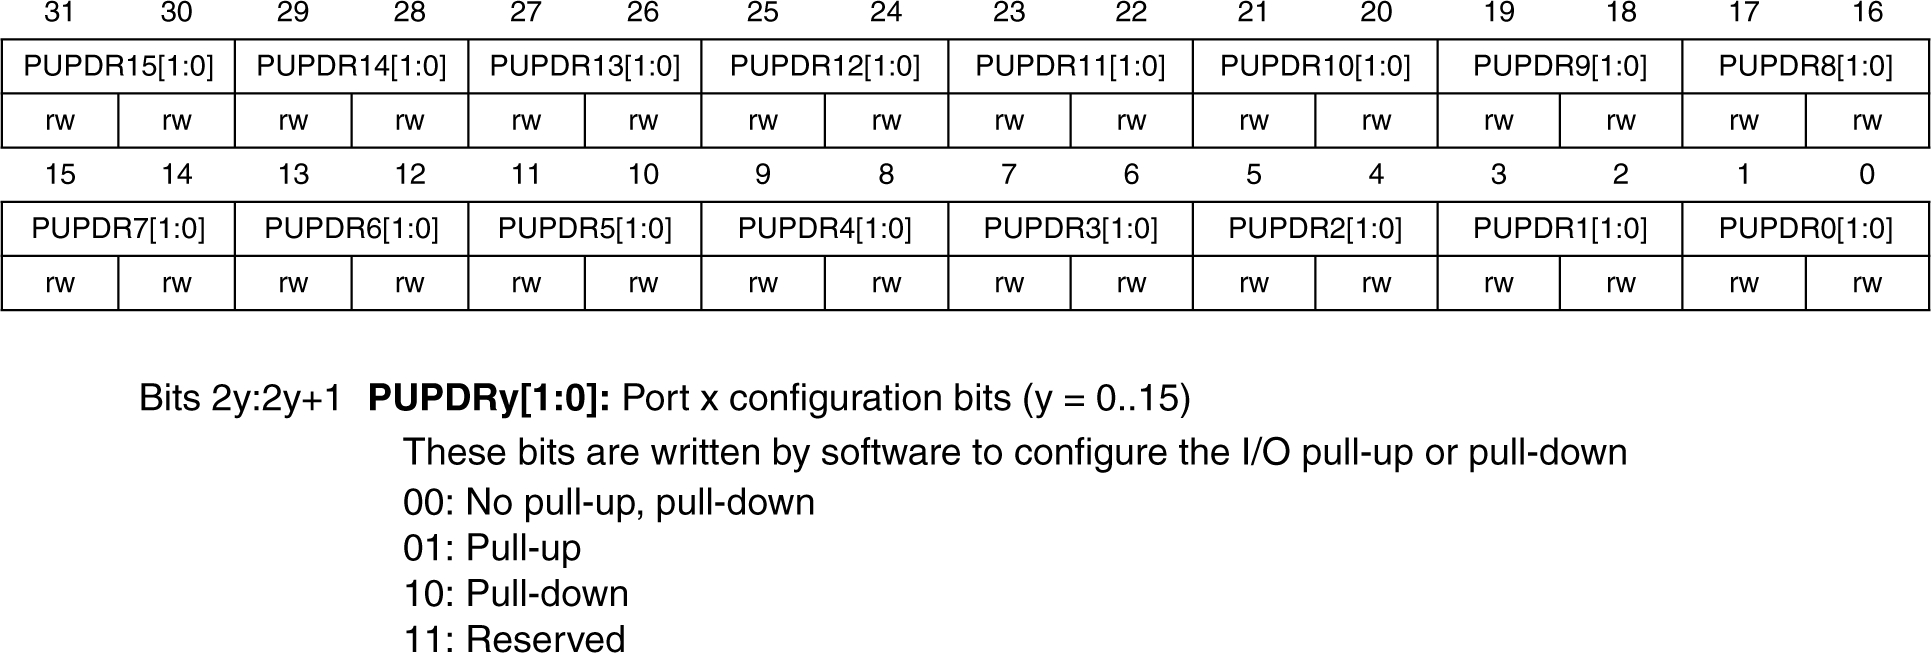
\includegraphics[scale=0.25]{Image/42.jpg} 
\end{center}
\caption{Регистр \textit{GPIOx\_PUPDR }(GPIO port pull-up/pull-down register)}
\end{figure}

\begin{verbatim}
GPIOA->PUPDR &= ~(GPIO_PUPDR_PUPDR1 | GPIO_PUPDR_PUPDR2 |
                  GPIO_PUPDR_PUPDR3 | GPIO_PUPDR_PUPDR8 | 
                  GPIO_PUPDR_PUPDR9 | GPIO_PUPDR_PUPDR10 | 
                  GPIO_PUPDR_PUPDR15);

// GPIOA->PUPDR &= ~0xC03F00FC;
// 0xC03F00FC = 1100 0000 0011 1111 0000 0000 1111 1100 
\end{verbatim}
Если необходимо отключить подтягивающие резисторы для всех пинов, можно записать в регистр значение:
\begin{verbatim}
GPIOA->PUPDR = 0x0;
\end{verbatim}

Для установки альтернативной функции для портов микроконтроллера используются два регистра \textit{GPIOx\_AFRL} (GPIO alternate function low register), отвечающий за младшие пины (с 0 по 7) и \textit{GPIOx\_AFRH} (GPIO alternate function high register), отвечающий за старшие пины (с 8 по 15). Все разряды регистров сгруппированы в группы \textit{AFRLy[3:0]} и \textit{AFRHy[3:0]}, где \textit{y} -- номер пина соответствующего порта. Порты должны быть настроены на использование альтернативной функции \textit{AF11}, для этого в группе, отвечающей за пин, должно быть установлено значение \verb\1011\.


\begin{figure}[H]
\begin{center}
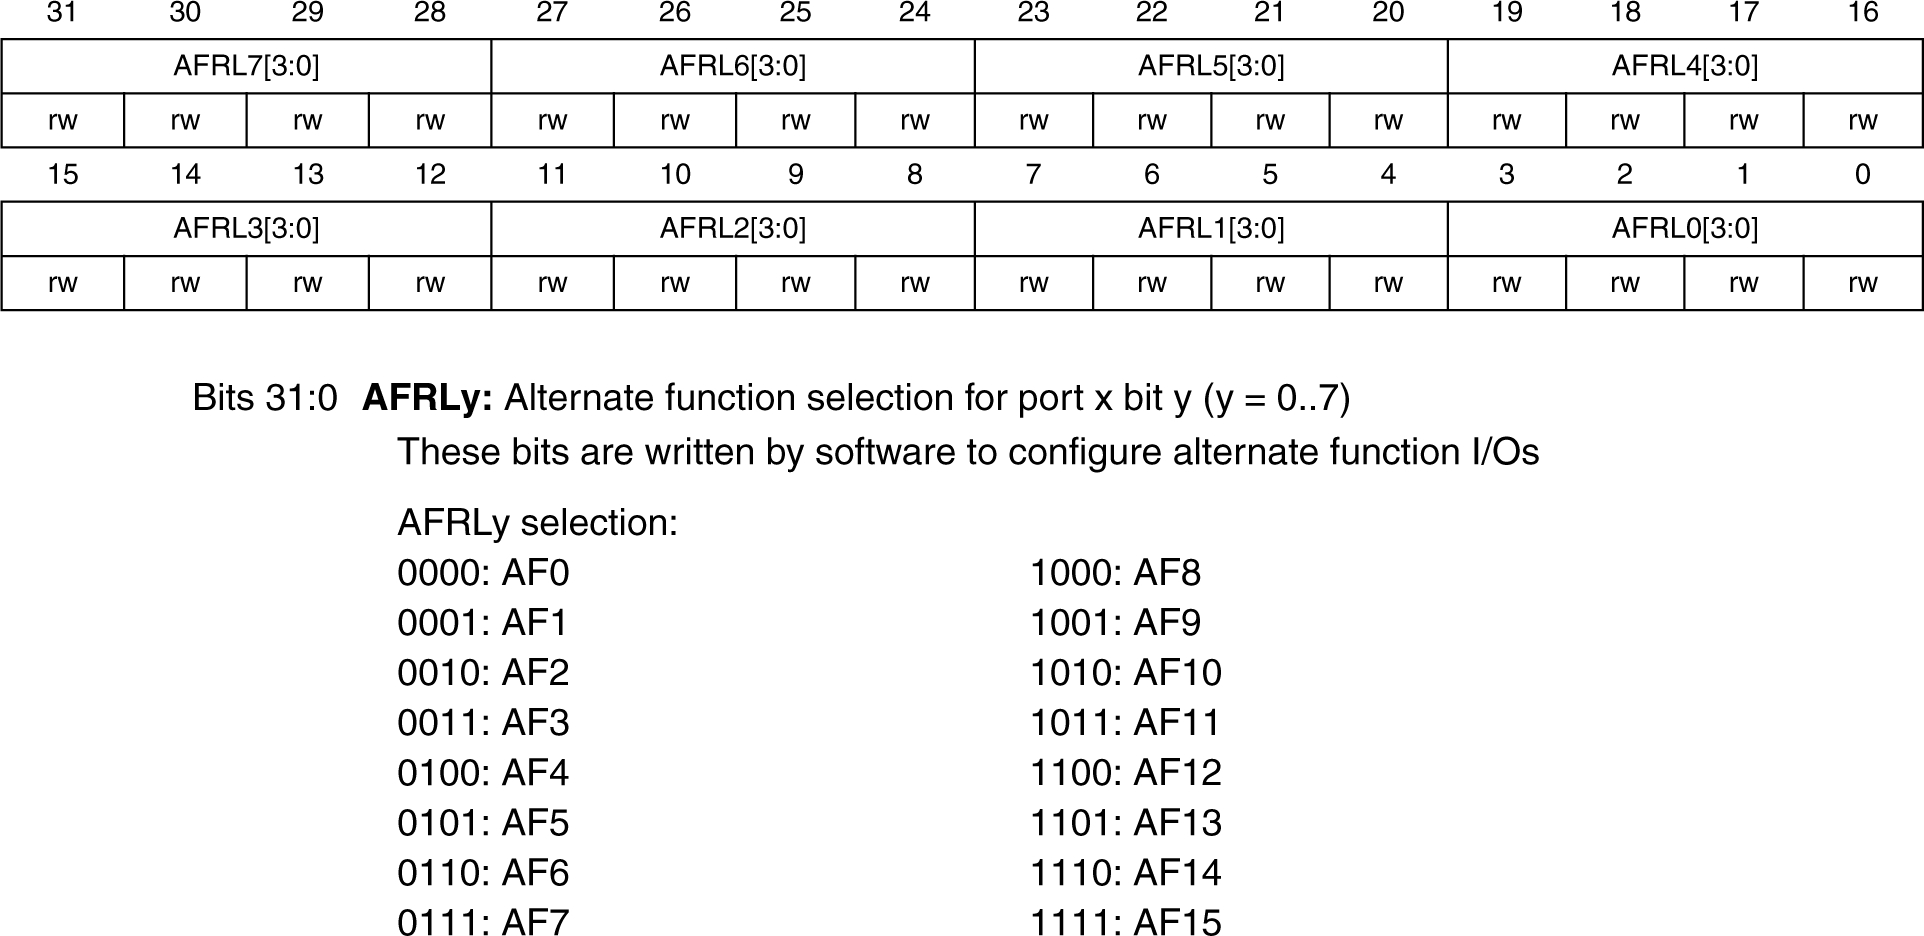
\includegraphics[scale=0.25]{Image/43.jpg} 
\end{center}
\caption{Регистр \textit{GPIOx\_AFRL} (GPIO alternate function low register)}
\end{figure}
\begin{figure}[H]
\begin{center}
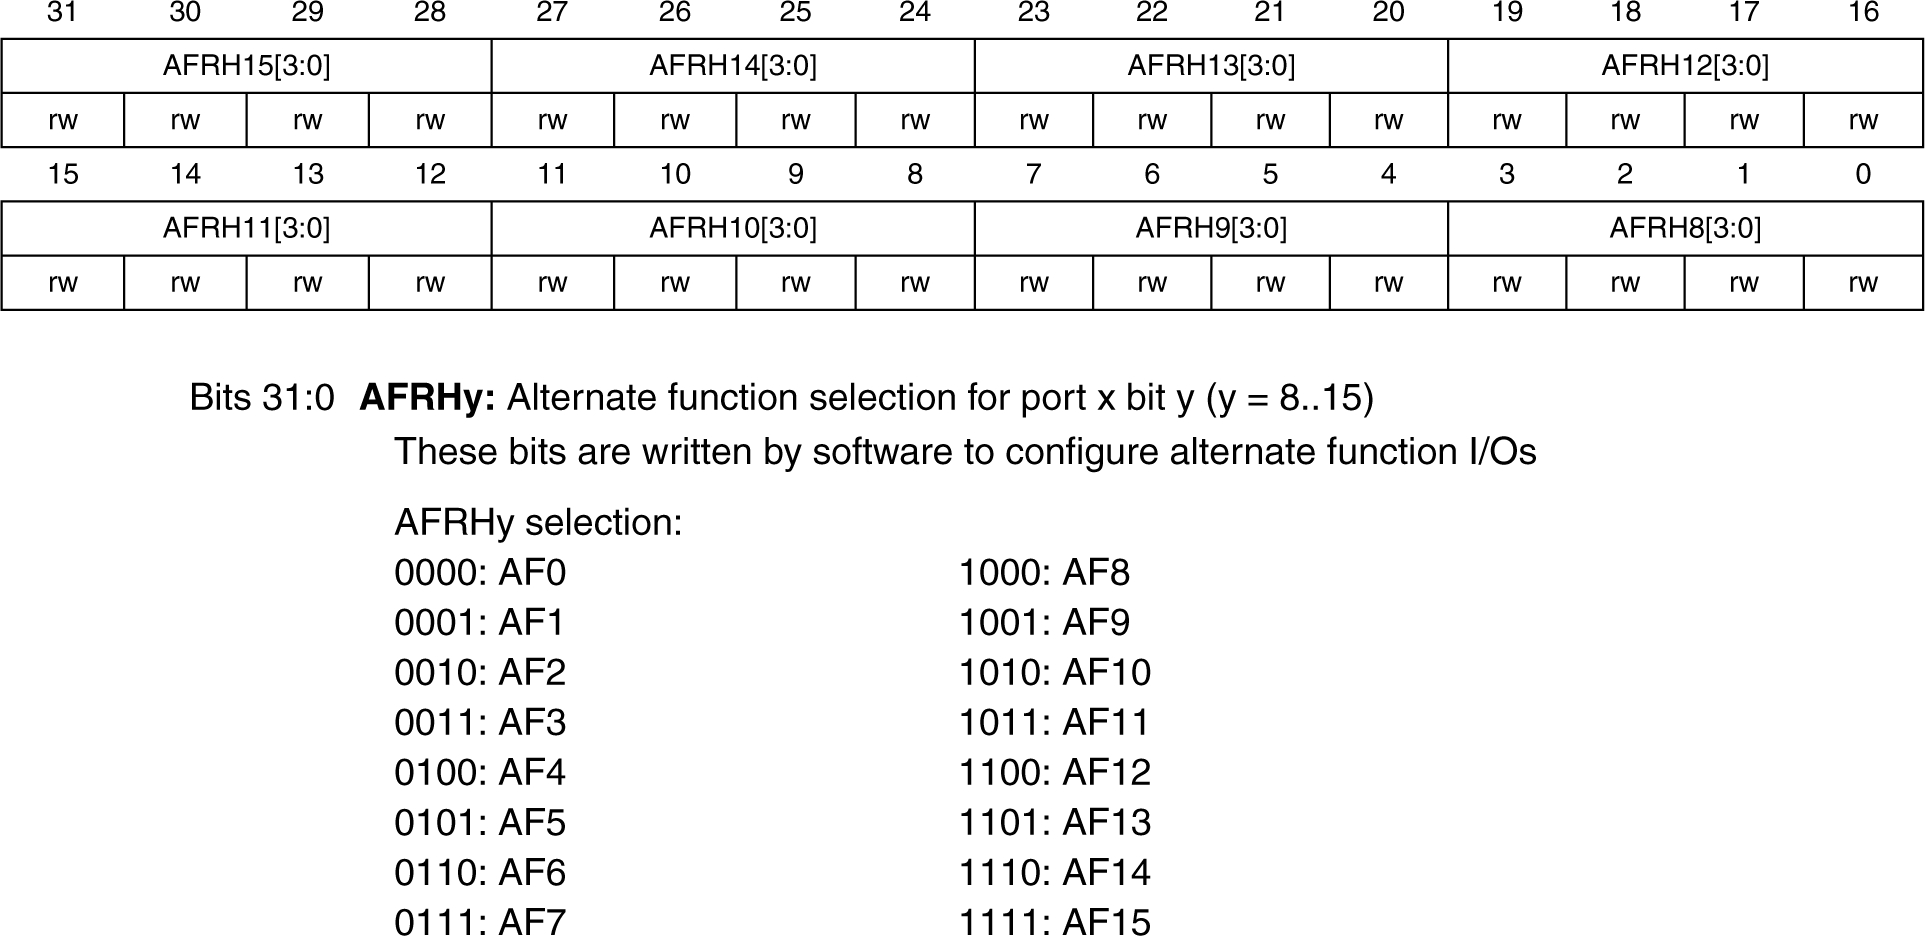
\includegraphics[scale=0.25]{Image/44.jpg} 
\end{center}
\caption{Регистр \textit{GPIOx\_AFRH} (GPIO alternate function high register)}
\end{figure}
Для этого необходимо записать в регистры значения:
\begin{verbatim}
GPIOA->AFR[0] = 0xBBB0;
// 0xBBB0 = 1011 1011 1011 0000_2 

GPIOA->AFR[1] = 0xB0000BBB;
// 0xB0000BBB = 1011 0000 0000 0000 0000 1011 1011 1011 
\end{verbatim}
\verb#AFR[0] = 0xBBB0# --- записывает значение в регистр \textit{GPIOx\_AFRL}.
\verb#AFR[1] = 0xB0000BBB# --- записывает значение в регистр \textit{GPIOx\_AFRH}.

Настройки соответствующих пинов портов \textit{GPIOB, GPIOC} производятся аналогично. Схема конфигурации порта приведена на рисунке \ref{portconf}. 

\begin{figure}[H]
\begin{center}
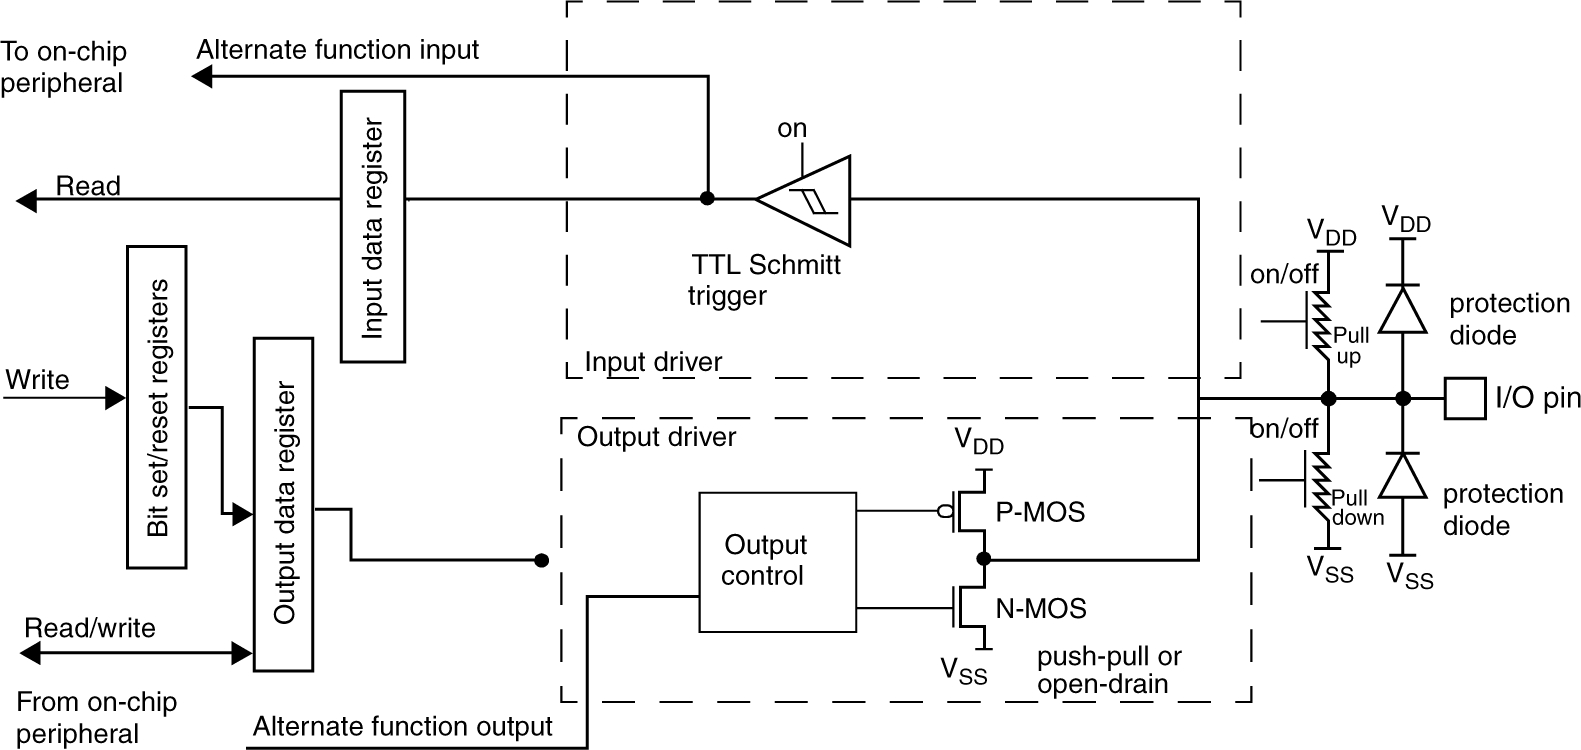
\includegraphics[scale=0.32]{Image/45.jpg} 
\end{center}
\caption{Схема конфигурации порта}\label{portconf}
\end{figure}


\section{Настройка контроллера ЖКИ}
При работе с контроллером ЖКИ, как и с другой периферией, на него необходимо подать тактовый сигнал. Тактовый сигнал также подается на систему управления питанием. Контроллер и система управления питанием для тактирования используют шину \textit{APB1}. Для разрешения тактирования в регистре \textit{RCC\_APB1ENR} (APB1 peripheral clock enable register) необходимо установить \verb\1\ в 9 и 28 разрядах.

\begin{figure}[H]
\begin{center}
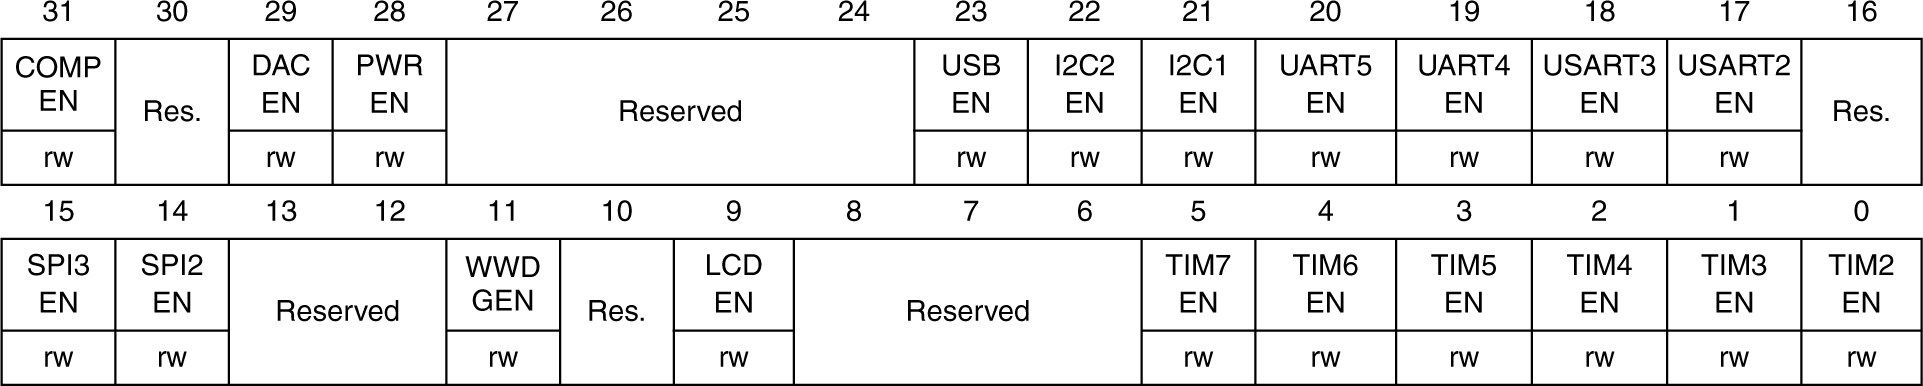
\includegraphics[scale=0.25]{Image/46.jpg} 
\end{center}
\caption{Регистр \textit{RCC\_APB1ENR} (APB1 peripheral clock enable register)}
\end{figure}

\begin{verbatim}
RCC->APB1ENR |= RCC_APB1ENR_PWREN|RCC_APB1ENR_LCDEN;

// RCC->APB1ENR |= 0x10000200;
// 0x10000200 = 1 0000 0000 0000 0000 0010 0000 0000 
\end{verbatim}

	Для работы контроллера ЖКИ необходимо указать источник тактовых сигналов. Источник указывается в регистре \textit{ RCC\_CSR}. По умолчанию запись в этот регистр запрещена. В регистре управления питанием  \textit{PWR\_CR} (PWR power control register) снимается защита от записи в регистр  \textit{RCC\_CSR}. Регистр  \textit{RCC\_CSR} управляет источниками тактирования часов  \textit{RTC }и контроллера ЖКИ.

\begin{figure}[H]
\begin{center}
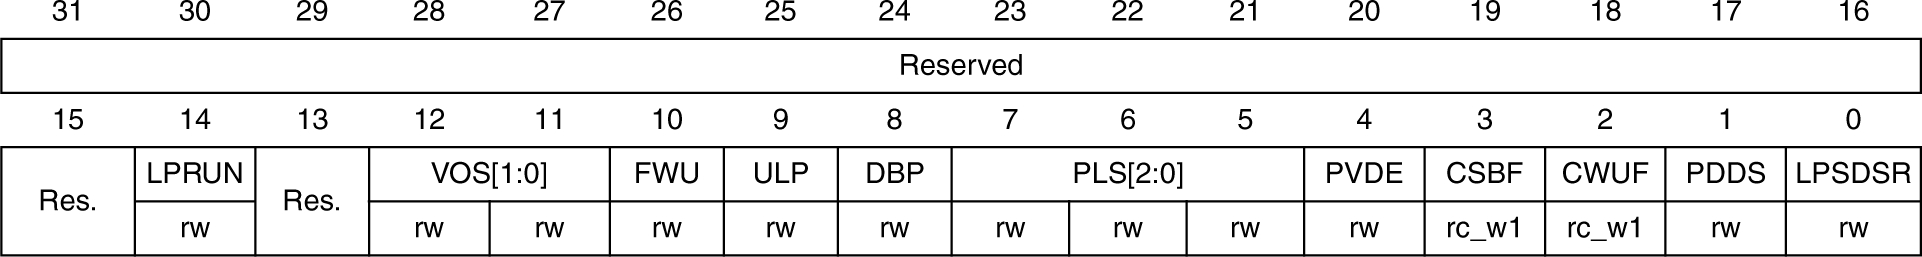
\includegraphics[scale=0.25]{Image/47.jpg} 
\end{center}
\caption{Регистр \textit{PWR\_CR} (PWR power control register)}
\end{figure}

Запись в регистр \textit{ RCC\_CSR} разрешается установкой \verb\1\ в 8 разряд регистра \textit{PWR\_CR}. 

\begin{verbatim}
PWR->CR |= PWR_CR_DBP; 

// PWR->CR |= 0x100;
// 0x100 = 1 0000 0000 
\end{verbatim}


Для смены источника тактирования контроллера ЖКИ (и часов RTC тоже) необходимо сначала выполнить сброс источника тактирования установкой бита \textit{RTCRST} (установкой \verb\1\ в 23 разряд) в регистре \textit{ RCC\_CSR} (Control/status register). 

\begin{figure}[H]
\begin{center}
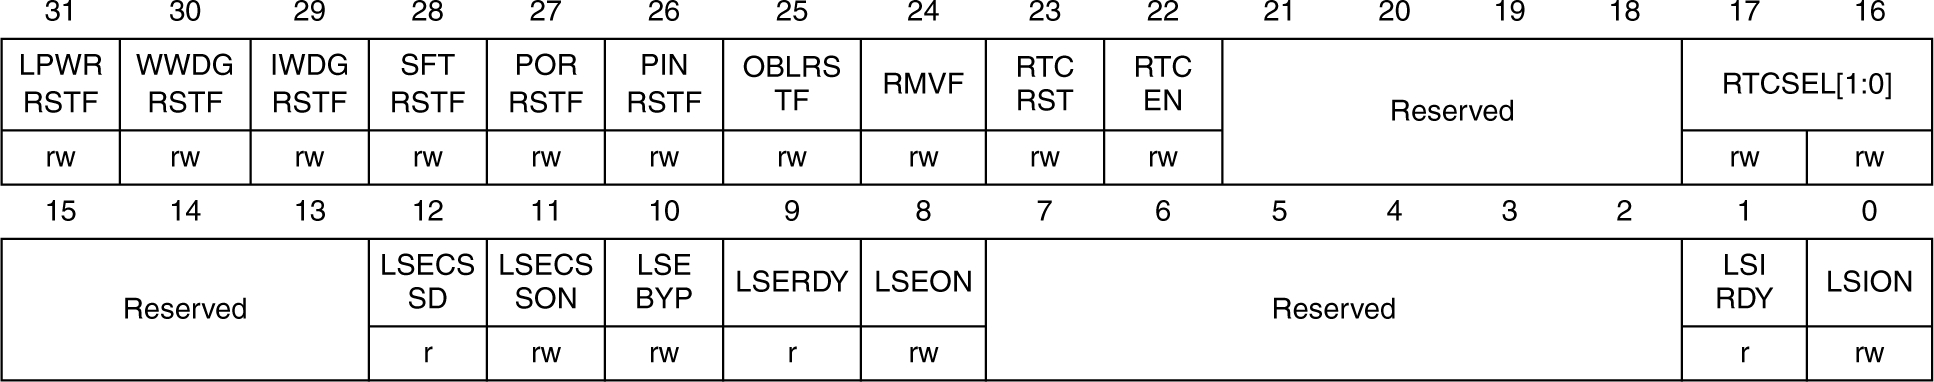
\includegraphics[scale=0.25]{Image/48.jpg} 
\end{center}
\caption{Регистр \textit{ RCC\_CSR}(Control/status register)}
\end{figure}

\begin{verbatim}
RCC->CSR |= RCC_CSR_RTCRST;

// RCC->CSR |= 0x800000;
// 0x800000 = 1000 0000 0000 0000 0000 0000 
\end{verbatim}
Для выбора нового источника тактирования необходимо убрать бит  \textit{RTCRST}:
\begin{verbatim}
RCC->CSR &= ~RCC_CSR_RTCRST;

// RCC->CSR &= ~0x800000;
\end{verbatim}
В качестве источника тактового сигнала выбирается внешний НЧ генератор. Для включения генератора в регистре \textit{ RCC\_CSR} необходимо установить бит \textit{LSEON} (установить \verb\1\ в 8 разряд):
\begin{verbatim}
RCC->CSR |= RCC_CSR_LSEON; 

// RCC->CSR |= 0x100; 
// 0x100 = 1 0000 0000
\end{verbatim}
После включения генератора необходимо некоторое время на его стабилизацию. Готовность генератора проверяется аппаратной установкой бита \textit{LSERDY} в регистре \textit{ RCC\_CSR}:
\begin{verbatim}
while(!(RCC->CSR&RCC_CSR_LSERDY));
\end{verbatim}
Выбор внешнего НЧ генератора в качестве источника тактового сигнала осуществляется установкой в группе \textit{RTCSEL[1:0]} регистра \textit{ RCC\_CSR} значения \verb\01\:
\begin{verbatim}
RCC->CSR |= RCC_CSR_RTCSEL_LSE;

// RCC->CSR |= 0x10000; 
// 0x10000 = 1 0000 0000 0000 0000
\end{verbatim}
В контроллере ЖКИ необходимо установить нужный режим \textit{bias}. Для этого в регистре \textit{LCD\_CR} (LCD control register) необходимо установить значение \verb\10\ в группу \textit{BIAS[1:0]}. Перед установкой бит необходимо очистить биты от <<мусора>>:
\begin{verbatim}
LCD->CR &= ~LCD_CR_BIAS;

// LCD->CR &= ~0x60;
\end{verbatim}
Выбор режима \textit{bias=1/3}:
\begin{verbatim}
LCD->CR |= LCD_CR_BIAS_1;

// LCD->CR |= 0x40;
\end{verbatim}
Устанавливаем режим \textit{duty=1/4}. Для этого также вначале сбрасываем все биты:
\begin{verbatim}
LCD->CR &=~LCD_CR_DUTY; 

// LCD->CR &= ~0x1C;
\end{verbatim}
Устанавливаем значение \verb\011\ в группу \textit{DUTY[1:0]} регистра \textit{LCD\_CR} для режима \textit{duty=1/4}:
\begin{verbatim}
LCD->CR |= LCD_CR_DUTY_0|LCD_CR_DUTY_1;

// LCD->CR |= 0xС;
\end{verbatim}

\begin{figure}[H]
\begin{center}
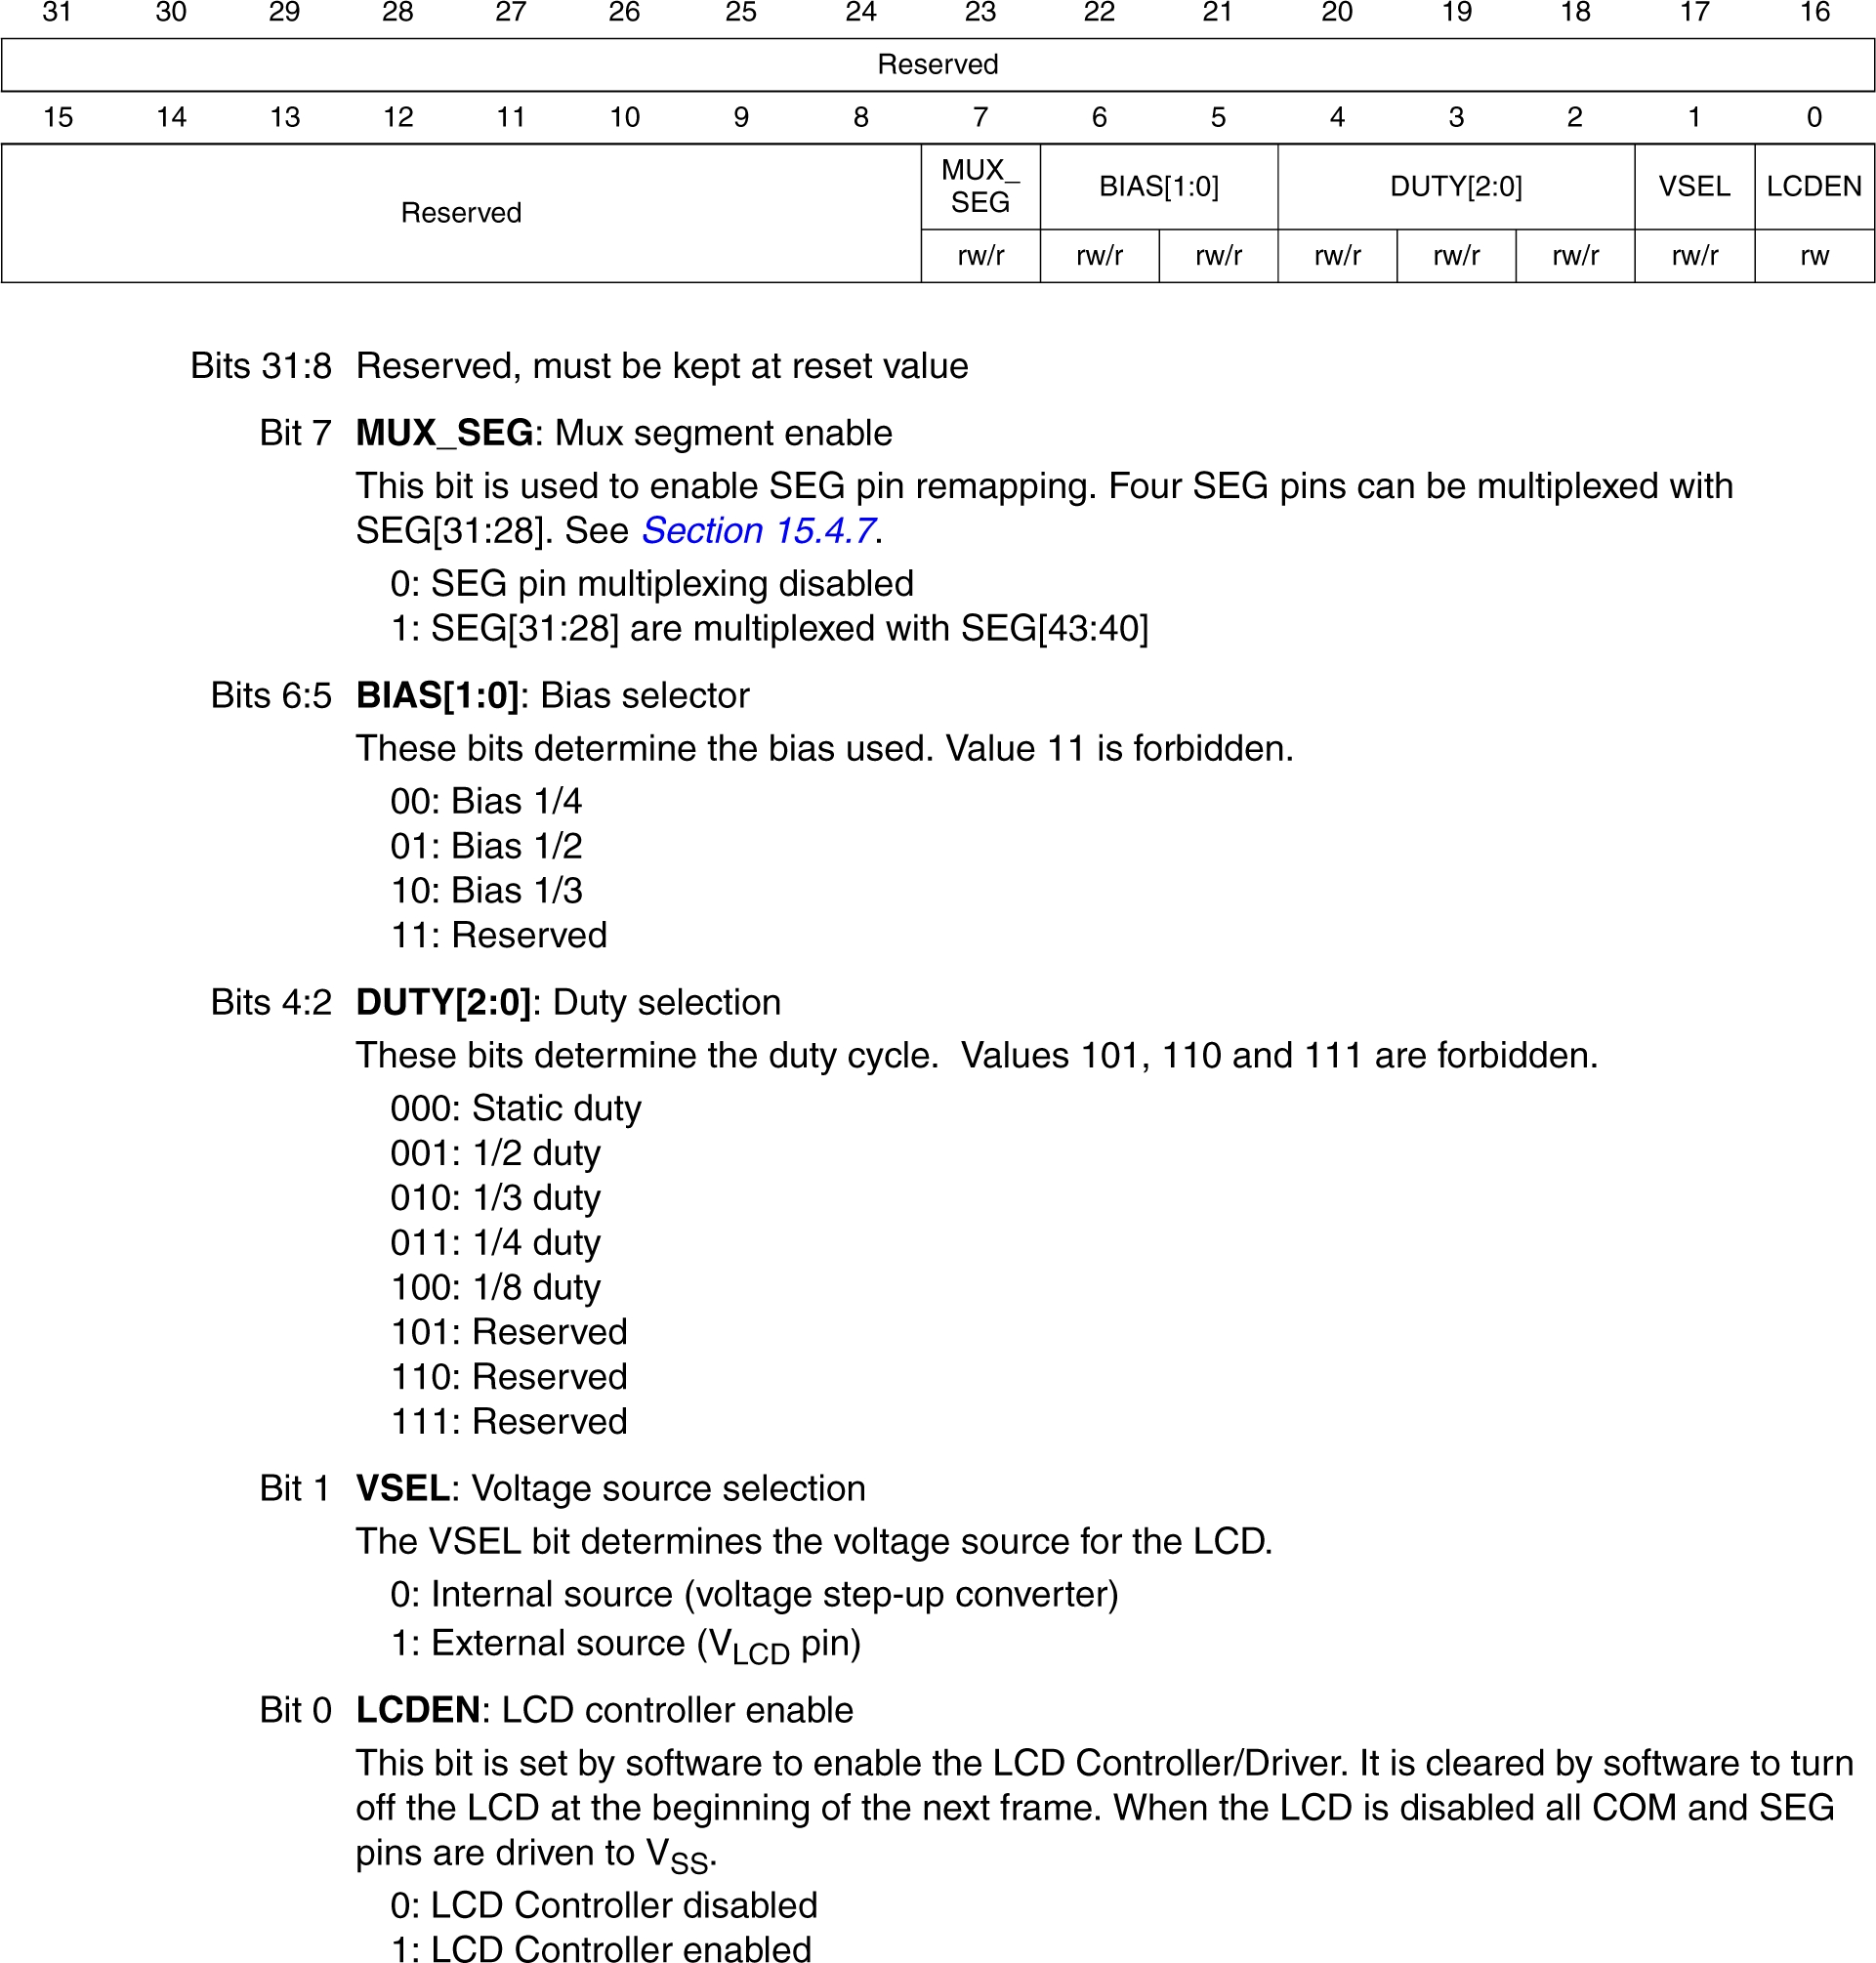
\includegraphics[scale=0.25]{Image/49.jpg} 
\end{center}
\caption{Регистр \textit{LCD\_CR} (LCD control register)}
\end{figure}
Активируем функцию переназначения выводов. Для этого устанавливаем \verb\1\ в 7 разряд регистра \textit{LCD\_CR}:
\begin{verbatim}
LCD->CR |= LCD_CR_MUX_SEG; 

// LCD->CR |= 0x80;
\end{verbatim}
Устанавливаем значения коэффициентов деления частоты тактового сигнала \textit{LCDCLK}. Значения коэффициентов выставляются в регистре \textit{LCD\_FCR} (LCD frame control register). Вначале также очищаем все биты, затем устанавливаем нужные. 
\begin{verbatim}
LCD->FCR &= ~LCD_FCR_PS;
LCD->FCR &= ~LCD_FCR_DIV;

// LCD->FCR &= ~0x3C00000;
// LCD->FCR &= ~0x3C0000;
\end{verbatim}
\begin{figure}[H]
\begin{center}
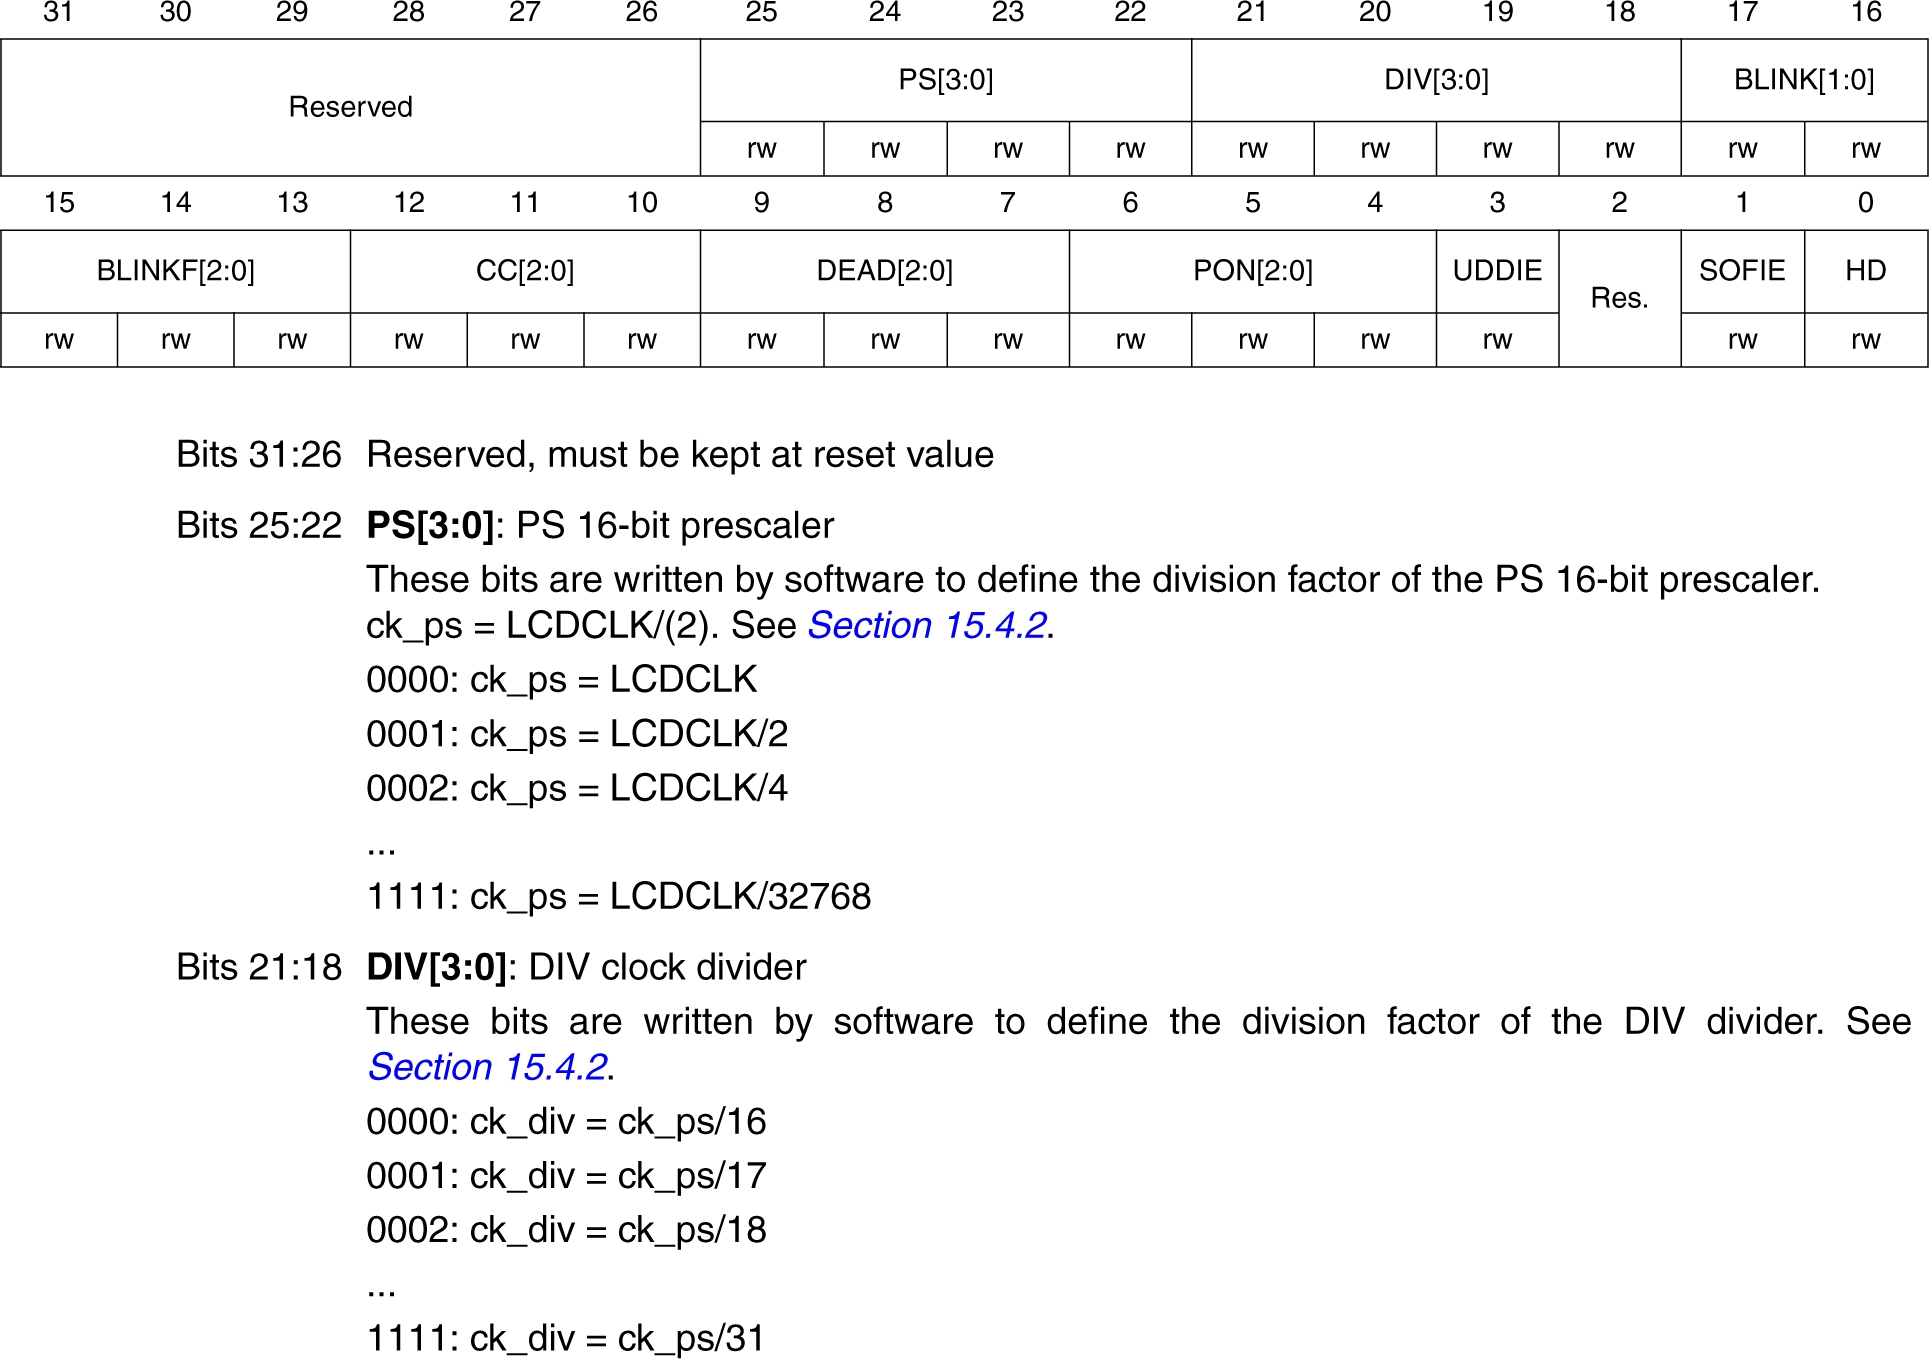
\includegraphics[scale=0.25]{Image/50.jpg} 
\end{center}
\caption{Регистр \textit{LCD\_FCR} (LCD frame control register)}
\end{figure}
Значения коэффициентов деления частоты тактового сигнала устанавливаем равными \textit{ck\_ps = LCDCLK/16, ck\_div = ck\_ps/17}. Для этого устанавливаем \verb\1\ в 24 и в 18 разряды.
\begin{verbatim}
LCD->FCR |= 0x1040000;
// 0x1040000 = 1 0000 0100 0000 0000 0000 0000 
\end{verbatim}
Частоту обновления кадров можно установить больше, например:
\begin{verbatim}
LCD->FCR &= ~0x3C0000;
\end{verbatim}
В это случае, при использовании библиотечных функций вывода изображений на ЖКИ, задержка обновления информации будет менее выражена, однако на ЖКИ будут видны артефакты.

Для установки нужного уровня контраста необходимо установить значение \verb\010\ в группу \textit{СС[1:0]}, так же предварительно очистив биты от старых значений:
\begin{verbatim}
LCD->FCR &= ~LCD_FCR_CC;  
LCD->FCR |= LCD_FCR_CC_1; 

// LCD->FCR &= ~0x1C00;
// LCD->FCR |= 0x800;
// 0x800 = 1000 0000 0000
\end{verbatim}
После установки всех значений необходимо некоторое время на синхронизацию регистра \textit{LCD\_FCR}. Синхронизация регистра проверяется аппаратной установкой бита \textit{FCRSF} в регистре \textit{LCD\_SR} (LCD status register).
\begin{verbatim}
while(!(LCD->SR&LCD_SR_FCRSR)); 
\end{verbatim}
\begin{figure}[H]
\begin{center}
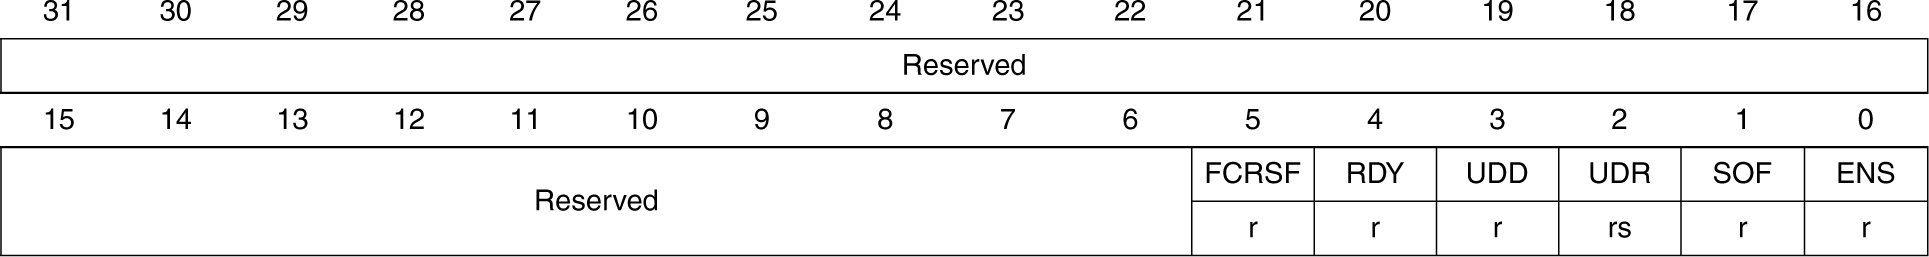
\includegraphics[scale=0.25]{Image/51.jpg} 
\end{center}
\caption{Регистр \textit{LCD\_SR} (LCD status register)}
\end{figure}
В качестве источника напряжения для ЖКИ выбираем внутренний \textit{step-up converter} для формирования \textit{V\_lcd}.  Для этого в первый разряд регистра \textit{LCD\_CR} (LCD control register) устанавливается значение \verb\0\:
\begin{verbatim}
LCD->CR &= ~LCD_CR_VSEL; 

//LCD->CR &= ~0x2;
\end{verbatim}
Разрешение работы ЖКИ контроллера происходит установкой \verb\1\ в 0 разряд регистра \textit{LCD\_CR} (LCD control register):
\begin{verbatim}
LCD->CR |= LCD_CR_LCDEN;

//LCD->CR |= 0x1;
\end{verbatim}
После установки в качестве источника напряжения внутреннего \textit{step-up converter}, необходимо дождаться его готовности. Готовность проверяется аппаратной установкой бита \textit{RDY} в регистре \textit{LCD\_SR} (LCD status register).
\begin{verbatim}
while(!(LCD->SR&LCD_SR_RDY)); 
\end{verbatim}
После разрешения работы контроллера ЖКИ, необходимо дождаться его готовности. Готовность проверяется аппаратной установкой бита \textit{ENS} в регистре \textit{LCD\_SR} (LCD status register).
\begin{verbatim}
while(!(LCD->SR&LCD_SR_ENS));
\end{verbatim}






\section{Формирование изображения на ЖКИ}



\subsection{Вывод информации на ЖКИ с использованием регистров \textit{LCD\_RAM}}
\begin{figure}[H]
\begin{center}
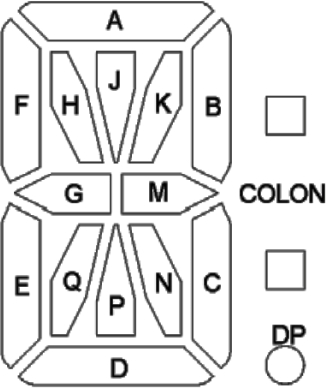
\includegraphics[scale=0.4]{Image/52.jpg} 
\end{center}
\caption{Обозначение сегментов}
\end{figure}
Все сегменты индикатора объединены в группы COM0 -- COM3 по 24 сегмента в каждой (SEG0 -- SEG23). Информация о сегментах хранится в регистрах \textit{LCD\_RAM} памяти контроллера ЖКИ. Разводка печатной платы такова, что номера сегментов не соответствуют номерам разрядов регистров \textit{LCD\_RAM}.

В качестве примера рассмотрим вывод на ЖКИ слова \verb#KAF403#.
\begin{figure}[H]
\begin{center}
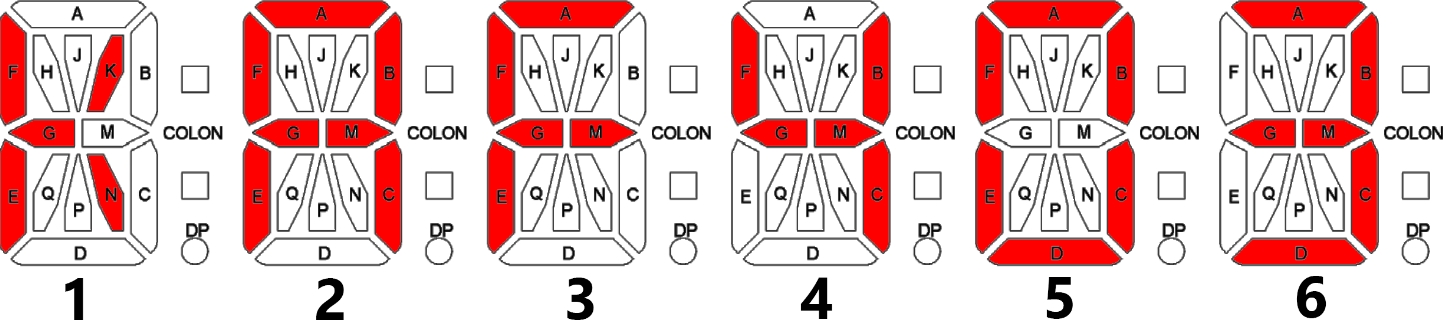
\includegraphics[scale=0.33]{Image/53.jpg} 
\end{center}
\caption{Вывод на ЖКИ}\label{kaf403}
\end{figure}
Для вывода данного слова необходимо (см. рисунок \ref{segment}) зажечь сегменты: 
\begin{itemize}
\item 1G, 1E, 2B, 2M, 2G, 2E, 3M, 3G, 3E, 4M, 4G, 5B, 5E, 6B, 6M, 6G принадлежащие группе COM0 (см. также рисунок \ref{SegmentTable});
\item 1F, 2A, 2F, 2C, 3A, 3F, 4F, 4C, 5A, 5F, 5C, 5D, 6A, 6C, 6D принадлежащие группе COM1;
\item 1K принадлежащие группе COM2;
\item 1N принадлежащие группе COM3;
\end{itemize}
Что бы зажечь выбранные сегменты, необходимо установиться 1 в соответствующих разрядах регистров \textit{LCD\_RAM}, принадлежащих определенной группе COM. Разряд регистра определяется в соответствии с таблицей \ref{SegmentTable}.  


\begin{table}[H]
\begin{center}
\caption{Таблица сегментов}\label{SegmentTable}
\begin{tabular}{|c|c|c|c|c|c|c|c|}
\hline
\multicolumn{6}{|c|}{\textbf{Сегменты ЖКИ}}                                                  & \multicolumn{2}{c|}{\textbf{Разряды}} \\ \hline
\textbf{COM3} & \textbf{COM2} & \textbf{COM1} & \textbf{COM0} & \textbf{Pin} & \textbf{Name} & \textbf{Pin}      & \textbf{Name}     \\ \hline
1N            & 1P            & 1D            & 1E            & 1            & LCDSEG0       & PA1               & SEG0              \\ \hline
1DP           & 1COLON        & 1C            & 1M            & 2            & LCDSEG1       & PA2               & SEG1              \\ \hline
2N            & 2P            & 2D            & 2E            & 3            & LCDSEG2       & PA3               & SEG2              \\ \hline
2DP           & 2COLON        & 2C            & 2M            & 4            & LCDSEG3       & PB3               & SEG7              \\ \hline
3N            & 3P            & 3D            & 3E            & 5            & LCDSEG4       & PB4               & SEG8              \\ \hline
3DP           & 3COLON        & 3C            & 3M            & 6            & LCDSEG5       & PB5               & SEG9              \\ \hline
4N            & 4P            & 4D            & 4E            & 7            & LCDSEG6       & PB10              & SEG10             \\ \hline
4DP           & 4COLON        & 4C            & 4M            & 8            & LCDSEG7       & PB11              & SEG11             \\ \hline
5N            & 5P            & 5D            & 5E            & 9            & LCDSEG8       & PB12              & SEG12             \\ \hline
BAR2          & BAR3          & 5C            & 5M            & 10           & LCDSEG9       & PB13              & SEG13             \\ \hline
6N            & 6P            & 6D            & 6E            & 11           & LCDSEG10      & PB14              & SEG14             \\ \hline
BAR0          & BAR1          & 6C            & 6M            & 12           & LCDSEG11      & PB15              & SEG15             \\ \hline
COM3          &               &               &               & 13           & LSDCOM3       & PB9               & COM3              \\ \hline
              & COM2          &               &               & 14           & LCDCOM2       & PA10              & COM2              \\ \hline
              &               & COM1          &               & 15           & LCDCOM1       & PA9               & COM1              \\ \hline
              &               &               & COM0          & 16           & LCDCOM0       & PA8               & COM0              \\ \hline
6J            & 6K            & 6A            & 6B            & 17           & LCDSEG12      & PA15              & SEG17             \\ \hline
6H            & 6Q            & 6F            & 6G            & 18           & LCDSEG13      & PB8               & SEG16             \\ \hline
5J            & 5K            & 5A            & 5B            & 19           & LCDSEG14      & PC0               & SEG18             \\ \hline
5H            & 5Q            & 5F            & 5G            & 20           & LCDSEG15      & PC1               & SEG19             \\ \hline
4J            & 4K            & 4A            & 4B            & 21           & LCDSEG16      & PC2               & SEG20             \\ \hline
4H            & 4Q            & 4F            & 4G            & 22           & LCDSEG17      & PC3               & SEG21             \\ \hline
3J            & 3K            & 3A            & 3B            & 23           & LCDSEG18      & PC6               & SEG24             \\ \hline
3H            & 3Q            & 3F            & 3G            & 24           & LCDSEG19      & PC7               & SEG25             \\ \hline
2J            & 2K            & 2A            & 2B            & 25           & LCDSEG20      & PC9               & SEG26             \\ \hline
2H            & 2Q            & 2F            & 2G            & 26           & LCDSEG21      & PC9               & SEG27             \\ \hline
1J            & 1K            & 1A            & 1B            & 27           & LCDSEG22      & PC10              & SEG40             \\ \hline
1H            & 1Q            & 1F            & 1G            & 28           & LCDSEG23      & PC11              & SEG41             \\ \hline

\end{tabular}
\end{center}
\end{table}


К примеру сегмент 1G подключен к выводу \textit{LCDSEG23} ЖКИ, за данный сегмент отвечает разряд \textit{SEG41}. Сегмент 1G принадлежит группе COM0 и за него отвечает разряд \textit{SEG41}, следовательно информация о нем должна быть записана в регистр \textit{LCD\_RAM[1]} (см. рисунок \ref{COM0}), но поскольку используется функция переназначения (remapping), то информация будет записана в разряд \textit{SEG29} регистра \textit{LCD\_RAM[0]} (см. страницу \pageref{RegMemLCD}). 

Сегмент 1Е подключен к выводу \textit{LSD\_SEG0} ЖКИ, за данный сегмент отвечает разряд \textit{SEG0}. Данный сегмент принадлежит группе COM0 и информация будет записана в регистр \textit{LCD\_RAM[0]}.

Сегмент 2B подключен к выводу \textit{LSD\_SEG20} ЖКИ, за данный сегмент отвечает разряд \textit{SEG26}. Данный сегмент принадлежит группе COM0 и информация будет записана в регистр \textit{LCD\_RAM[0]}.

Сегмент 2M подключен к выводу \textit{LSD\_SEG3} ЖКИ, за данный сегмент отвечает разряд \textit{SEG7}. Данный сегмент принадлежит группе COM0 и информация будет записана в регистр \textit{LCD\_RAM[0]}.

Сегмент 2G подключен к выводу \textit{LSD\_SEG21} ЖКИ, за данный сегмент отвечает разряд \textit{SEG27}. Данный сегмент принадлежит группе COM0 и информация будет записана в регистр \textit{LCD\_RAM[0]}.

Сегмент 2E подключен к выводу \textit{LSD\_SEG2} ЖКИ, за данный сегмент отвечает разряд \textit{SEG2}. Данный сегмент принадлежит группе COM0 и информация будет записана в регистр \textit{LCD\_RAM[0]}. 

Сегмент 1K подключен к выводу \textit{LSD\_SEG22} ЖКИ, за данный сегмент отвечает разряд \textit{SEG40}. C использованием функции переназначения информация должна быть записана в разряд \textit{SEG28}. 

Данный сегмент принадлежит группе COM2 и информация будет записана в регистр \textit{LCD\_RAM[4]}. 
Разряды для других сегментов определяются аналогично.

Далее исходя из полученных разрядов формируется двоичный код, который состоит из 1 в тех разрядах, которые соответствуют определенным ранее \textit{SEGx}. Полученный код записывается также в определенные ранее \textit{LCD\_RAM[x]}. В данной примере регистр \textit{LCD\_RAM[4]} (принадлежащий группе COM2) отвечает только за один сегмент 1K, 1 будет стоять в 28 разряде. В данный регистр будет записан следующий код:
\begin{verbatim}
LCD->RAM[4] = 0x10000000;
// 1 0000 0000 0000 0000 0000 0000 0000 = 0X1000 0000
\end{verbatim}
До записи значений в регистры памяти необходимо проверить завершена ли предыдущая передача данных на ЖКИ. Для этого проверяется бит \textit{UDR} (Update display request) регистра \textit{LCD\_SR} (LCD status register). Контроллер ЖКИ имеет два выходных буфера, информация заносится в первый буфер, а выводится на ЖКИ из второго буфера. Бит \textit{UDR} устанавливается во время передачи из первого буфера во второй, защищая от записи регистры \textit{LCD\_RAM}.
\begin{verbatim}
while(LCD->SR & LCD_SR_UDR);
\end{verbatim}
После записи информации в регистры \textit{LCD\_RAM} необходимо установить бит \textit{UDR} в регистре \textit{LCD\_SR} (LCD status register) (установить \verb\1\ во 2 разряд):
\begin{verbatim}
LCD->SR |= LCD_SR_UDR;

// LCD->SR |= 0x4;
// 0x4 = 100
\end{verbatim}

\subsection{Вывод информации на ЖКИ с использованием библиотеки}
В составе \textit{Standard Peripheral Library} (SPL) есть библиотека для работы с LCD дисплеями, состоящая из двух файлов \verb\stm32l1xx_lcd.c\ и \verb\stm32l1xx_lcd.h\. Инициализация контроллера происходит аналогично инициализации портов микроконтроллера в первой лабораторной работе, при помощи структуры. 
\begin{verbatim}
LCD_InitTypeDef LCD_InitStruct; 
LCD_InitStruct.LCD_Prescaler = LCD_Prescaler_1;
LCD_InitStruct.LCD_Divider = LCD_Divider_31;
LCD_InitStruct.LCD_Duty = LCD_Duty_1_4;
LCD_InitStruct.LCD_Bias = LCD_Bias_1_3;
LCD_InitStruct.LCD_VoltageSource = LCD_VoltageSource_Internal;
  
  /* Initialize the LCD */
LCD_Init(&LCD_InitStruct);
LCD_MuxSegmentCmd(ENABLE);  

  /* To set contrast to mean value */
LCD_ContrastConfig(LCD_Contrast_Level_4);

  /* Wait Until the LCD FCR register is synchronized */
LCD_WaitForSynchro();  

  /* Enable LCD peripheral */
LCD_Cmd(ENABLE);  

 /* Wait Until the LCD is enabled */
while(LCD_GetFlagStatus(LCD_FLAG_ENS) == RESET);

  /*!< Wait Until the LCD Booster is ready */ 
while(LCD_GetFlagStatus(LCD_FLAG_RDY) == RESET);

 // LCD_BlinkConfig(LCD_BlinkMode_Off,LCD_BlinkFrequency_Div32);      
LCD_GLASS_Clear();
\end{verbatim}

Стоит отметить, что перед вызовом функции
\begin{verbatim}
void LCD_Init(LCD_InitTypeDef* LCD_InitStruct)
\end{verbatim}
на контроллер ЖКИ необходимо подать тактовый сигнал.

В комплексе с отладочной платой STM32L-Discovery идет демонстрационная прошивка \textit{STM32L\_Discovery\_Firmware\_Pack}, которая также доступна вместе с исходными кодами и библиотеками на официальном сайте STMicroelectronics. В прошивку входят файлы \verb\stm32l_discovery_lcd.c\, \verb\stm32l_discovery_lcd.h\, \verb\discover_board.h\, в которых предоставлен набор удобных функций для работы с ЖКИ, установленным на отладочной плате STM32L-Discovery:

\begin{verbatim}
void LCD_bar(void);
void LCD_GLASS_Init(void);

//Вывод символа в определенном разряде
void LCD_GLASS_WriteChar(uint8_t* ch, bool point, bool column,uint8_t position);

//Вывод строки символов
void LCD_GLASS_DisplayString(uint8_t* ptr);
void LCD_GLASS_DisplayStrDeci(uint16_t* ptr);
void LCD_GLASS_ClearChar(uint8_t position);

//Очистка ЖКИ
void LCD_GLASS_Clear(void);

//Бегущая строка
void LCD_GLASS_ScrollSentence(uint8_t* ptr, uint16_t nScroll, 
                              uint16_t ScrollSpeed);
void LCD_GLASS_WriteTime(char a, uint8_t posi, bool column);
\end{verbatim}
% \chapter{Лабораторная работа №3. Знакомство с сенсорной панелью. Работа с прерываниями}

Цель работы: 
\begin{itemize}
\item Знакомство с существующими технологиями емкостных сенсорных панелей.
\item Настройка и использование стандартной библиотеки по работе с сенсорной панелью.
\item Изучение принципов работы с прерываниями.
\end{itemize}

\section{Описание принципов работы сенсорной панели}
На отладочной плате STM32L-Discovery установлена сенсорная панель, выполненная по емкостной технологии. Существует несколько технологий емкостных сенсорных датчиков \cite{appnote}

\textit{Измерение времени заряда/разряда RC-цепи} (RC acquisition principle) --- при касании в чувствительной зоне кнопки (чаще всего касание одного из электродов) изменяется емкость, соответственно изменяется постоянная времени цепи, изменение которой регистрируется контролирующей схемой. 
	
	\textit{Опрос датчика путем переноса заряда} (Charge transfer acquisition principle) --- опрос кнопки путем измерения времени заряда измерительного конденсатора разрядом конденсатора, образованного сенсорной кнопкой. В этом случае конденсатор сенсорной кнопки периодически заряжается, а его разряд происходит на другой конденсатор (измерительный, sampling capacitor), и замеряется время его заряда до определенного \textit{порогового напряжения (threshold voltage}). При касании кнопки ее емкость увеличивается (накапливается больший заряд), и заряд измерительного конденсатора происходит за меньшее время.   
	
	\textit{Технология поверхностной емкости }(Surface capacitance). Емкость кнопки изменяется при приближении пальца близко к ее поверхности за счет дополнительной емкости: 
\begin{itemize}
\item До земли через тело человека;
\item Емкости между человеческой рукой и устройством;
\item Емкости между телом человека и печатной платой устройства (наподобие антенны).
\end{itemize}
\begin{figure}[H]
\begin{center}
\includegraphics[scale=0.25]{Image/55.jpg} 
\end{center}
\caption{Принцип поверхностной емкости}
\end{figure}

\textit {Cx} --- паразитная емкость электрода.
 
\textit {Cf} --- обратная связь между землей и приложением.

\textit {Ct} --- емкость образованная касанием пальца.

\textit{Проекционная емкость (Projected capacitance)}. При прикосновении изменяется диэлектрическая проницаемость, соответственно изменяется общая емкость.

\section{Опрос датчика путем переноса заряда}

Данный метод является простым и наиболее удобным способом измерения емкости. Суть технологии заключается в том, что все GPIO, подключенные к сенсорной панели (кнопке) объединены в группы по 2 -- 4 порта в каждой. В каждой группе один GPIO выделен для \textit{измерительного конденсатора} (sampling capacitor). Остальные GPIO выделены для электродов и называются \textit{каналами} (channels).

\begin{figure}[H]
\begin{center}
\includegraphics[scale=0.5]{Image/56.jpg} 
\end{center}
\caption{Объединение портов в группы}\label{PortInGroup}
\end{figure}

Принцип переноса заряда состоит в накоплении заряда на конденсаторе \textit{Cx} и его разряде через измерительный конденсатор \textit{Cs}. Разряд повторяется до тех пор, пока напряжение на измерительном конденсаторе \textit{Cs} не достигнет определенного порогового уровня (threshold voltage). В таблице \ref{PerenosZaryada} приведен пример использования технологии опроса датчика путем переноса заряда для первого канала (G1\_IO1), подключенного к кнопке 1. Состояния с 3 по 7 повторяются до тех пор, пока напряжение на измерительном конденсаторе не достигнет порогового значения.


\begin{figure}[H]
\begin{center}
\includegraphics[scale=0.5]{Image/57.jpg} 
\end{center}
\caption{Схема подключения кнопок}
\end{figure}

\begin{figure}[H]
\begin{center}
\includegraphics[scale=0.7]{Image/58.jpg} 
\end{center}
\caption{Рост напряжения на измерительном конденсаторе \textit{Cs}}
\end{figure}



\begin{table}[H]
\caption{Опроса датчика путем переноса заряда. Принцип работы}\label{PerenosZaryada}
\begin{center}
\begin{tabular}{|c|>{\centering}m{2cm}|c|>{\centering}m{2cm}|c|c|>{\centering\arraybackslash}m{3cm}|}
\hline
Состояние & Ключ S1 & Ключ S2 & Ключ S3 & Ключ S4 & Ключ S5 & Описание\\
\hline
1 & Открыт & Закрыт & Открыт & Закрыт & Закрыт & Конденсаторы \textit{Cx1, Cx2, Cs} разряжены\\
\hline
2 & Открыт & Открыт & Открыт & Открыт & Открыт & Время простоя (Dead time)\\
\hline
3 & Закрыт & Открыт & Открыт & Открыт & Открыт & Заряд конденсатора \textit{Cx1}\\
\hline

4 & Открыт & Открыт & Открыт & Открыт & Открыт & Время простоя (Dead time)\\
\hline
5 & Открыт & Открыт & Открыт & Закрыт & Открыт & Разряд через конденсатор \textit{Cs}\\
\hline
6 & Открыт & Открыт & Открыт & Открыт & Открыт & Время простоя (Dead time)\\
\hline
7 &Открыт & Открыт & Открыт & Открыт & Открыт & Измерение напряжения на конденсаторе \textit{Cs}\\
\hline
\end{tabular}
\end{center}
\end{table}

%%%%%%%%%%%%%%%%%%%%%%%%%%%%%%%%%%%%%%%%%%%%%%%%%%%%%%%%%%%%%%%%%%%%%%%%%%%%%%%%%%%%%%%%%%%%


%%% Дописать




%%%%%%%%%%%%%%%%%%%%%%%%%%%%%%%%%%%%%%%%%%%%%%%%%%%%%%%%%%%%%%%%%%%%%%%%%%%%%%%%%%%%%%%%%%%%%%%%%%%%

\section{Типы сенсорных панелей (кнопок)}
Существует два типа сенсорных панелей (кнопок) --- \textit{многоканальные} и \textit{одноканальные}. Одноканальные сенсорные кнопки являются наиболее простым типом кнопок, имеющими всего два состояния -- нажата и не нажата. Примером многоканальных сенсорных кнопок являются линейный \textit{сенсорный датчик} (Normal patterned linear sensor), \textit{чересстрочный линейный сенсорный датчик} (Interlaced linear sensor) или \textit{ротационный сенсорный датчик} (Rotary sensor).
\begin{figure}[H]
\begin{center}
\includegraphics[scale=0.25]{Image/59.jpg} 
\end{center}
\caption{Чересстрочный линейный сенсорный датчик (Interlaced linear sensor)}
\end{figure}

\begin{figure}[H]
\begin{center}
\includegraphics[scale=0.25]{Image/60.jpg} 
\end{center}
\caption{Ротационный сенсорный датчик (Rotary sensor)}
\end{figure}

Многоканальные кнопки подключаются к нескольким группам GPIO и используют несколько каналов, подключенных к измерительным конденсаторам. Интерполяция сигналов между каналами позволяет определять положение касания сенсорной панели. Более подробное описание методов измерения емкости и принципов построения сенсорных панелей приведено в документации \textit{Application note AN2869}.

\section{Библиотека \textit{Touch --  Sensing Library} (TSL)}
\subsection{Описание библиотеки \textit{Touch --  Sensing Library} (TSL)}

Для работы с сенсорными панелями ST Microelectronics разработала библиотеку \textit{Touch --  Sensing Library} --- аналог \textit{Standard Peripherals Library} для работы с периферией. Библиотека позволяет организовывать не только опрос емкостных сенсоров, но и реализуют обработку сигналов с целью снижения влияния внешних помех и повышения стабильности работы. 
	
	 Библиотеки \textit{STM8/STM32 Touch --  Sensing Library} предоставляется в виде открытых исходных кодов на языке С, совместимых со всеми популярными компиляторами (MISRA, Cosmic, IAR, Raisonance C) с примерами использования. Структура библиотек для 8- и 32-битных микроконтроллеров практически идентична -- набор высокоуровневых функций для взаимодействия с прикладными программами, набор вспомогательных сервисов, драйвера устройств, специфичные для каждого из семейств контроллеров, и ядро библиотеки, отвечающее за обработку информации от сенсорных кнопок, калибровку, фильтрацию сигналов, отслеживание изменения окружения. 

Кроме опроса емкостной кнопки в библиотеке предусмотрены алгоритмы обработки сигнала, позволяющие компенсировать негативное влияние таких факторов, как температура, внешнее окружение, изменение напряжения питания. 
 	
 	Ядром библиотеки являются два конечных автомата -- \textit{центральный автомат} (Main State Machine), управляющий последовательностью выполнения действий, и \textit{автомат сенсорной кнопки} (Key State Machine), отслеживающий изменения ее состояния, копия которого запускается для каждой из установленных кнопок.


\begin{figure}[h!]
\begin{center}
\includegraphics[scale=0.6]{Image/61.jpg} 
\end{center}
\caption{Структура библиотеки \textit{Touch --  Sensing Library}}
\end{figure}

Интерфейс программирования приложений (API, application programming interface) библиотеки доступен через заголовочный файл  \verb\stm32_tsl_api.h\, который содержит описание всех API функций, переменных и структур. Для работы библиотеки используются две функции, которые позволяют инициализировать и запустить центральный автомат:

\verb#TSL_Init()# --- функция вызывается один раз и проводит полную инициализацию системы.

\verb#TSL_Action()# --- функция вызывается периодически в процессе выполнения программы.

Состояния центрального автомата (Main State Machine) хранятся в переменной  \verb\TSLState\ перечисляемого типа \verb\TSLState_T\, определенного в \verb\stm32_tsl_api.h\, а состояния и параметры кнопок хранятся в массиве структур:

\verb#sSCKeyInfo[]# --- для одноканальных кнопок (Single\_Channel\_Complete\_Info\_T type).

\verb#sMCKeyInfo[]# --- для многоканальных кнопок (Tria\_Channel\_Complete\_Info\_T type).

Ядро библиотеки \textit{Touch --  Sensing Library} состоит из следующих файлов:
\begin{itemize}
\item \verb\stm32_tsl_singlechannelkey.c\, \verb\stm32_tsl_singlechannelkey.h\ --- эти файлы содержат функции управления центральным автоматом для одноканальных кнопок и другие функции, выделенные для этого типа кнопок.
\item \verb\stm32_tsl_multichannelkey.c\, \verb\stm32_tsl_multichannelkey.h\ --- эти файлы содержат функции управления центральным автоматом для многоканальных кнопок и другие функции, выделенные для этого типа кнопок, например, вычисление положения нажатия на сенсорную панель.

\item \verb\stm32_tsl_services.c\, \verb\stm32_tsl_services.h\ --- содержат функции, необходимы для кнопок обоих типов.

\item \verb\stm32_tsl_internal.h\ --- файл содержит прототипы функций и макросы для работы TSL
\end{itemize}



\subsection{Центральный автомат}
Центральный автомат (Main State Machine) управляет последовательностью действий, выполняемых системой.  Автомат определен в функции \verb\TSL_Action()\. Элементами перечисляемого типа \verb\TSLState_T\ являются целочисленные константы, отображающие состояния автомата:

\begin{itemize}
\item \verb\TSL_IDLE_STATE\ --- стабильное состояние, в котором все действия завершены. Данное состояние всегда присутствует. Используется для синхронизации TSL с программой.

\item \verb\TSL_SCKEY_P1_ACQ_STATE\ --- перенос заряда от первой группы одноканальных кнопок (first bank acquisition). Данное состояние всегда присутствует.

\item \verb\TSL_SCKEY_P1_PROC_STATE\ --- обработка информации от первой группы одноканальных кнопок (first bank signal processing). Данное состояние всегда присутствует.

\item \verb\TSL_SCKEY_P2_ACQ_STATE\ --- перенос заряда от второй группы одноканальных кнопок (second bank acquisition).

\item \verb\TSL_SCKEY_P2_PROC_STATE\ --- обработка информации от второй группы одноканальных кнопок (second bank signal processing).

\item \verb\TSL_SCKEY_P3_ACQ_STATE\ --- перенос заряда от третьей группы одноканальных кнопок (third bank acquisition).

\item \verb\TSL_SCKEY_P3_PROC_STATE\ ---  обработка информации от третьей группы одноканальных кнопок (third bank signal processing).

\item \verb\TSL_MCKEY1_ACQ_STATE\ --- перенос заряда первой многоканальной кнопки.

\item \verb\TSL_MCKEY2_ACQ_STATE\ --- перенос заряда второй многоканальной кнопки.

\item \verb\TSL_MCKEY_PROC_STATE\ --- обработка сигналов от первой и второй многоканальных кнопок.

\item \verb\TSL_ECS_STATE\ --- Environment Control System process. Это состояние всегда присутствует.
\end{itemize}

Все дополнительные состояние инициализируются в файле \verb\stm32_tsl_conf.h\.
\begin{figure}[h!]
\begin{center}
\includegraphics[scale=0.45]{Image/62.jpg} 
\end{center}
\caption{Граф центрального автомата (Main State Machine)}
\end{figure}


\subsection{Фильтры устранения дребезга (Debounce Filters)}

\textit{Debouncing} --- устранение дребезга. Данный фильтр позволяет фиксировать нажатие на сенсорную панель (кнопку) только в случае, если кнопка нажата в течение нескольких циклов работы центрального автомата. Количество циклов определяется пользователем во время настройки фильтра в файле \verb\stm32_tsl_conf.h\. Фильтр помогает устранить эффект дребезга контактов, позволяя фиксировать только истинное нажатие. Фильтр используется при обнаружении нажатия (key detection), обнаружении конца нажатия (key end detection) и до входа в состоянии калибровки (calibration state). Счетчик, отвечающий за количество циклов, устанавливается в состоянии инициализации и уменьшается каждый цикл центрального автомата. Для установки счетчика определены три константы в файле конфигурации \verb\stm32_tsl_conf.h\:
\begin{itemize}
\item \verb\DETECTION_INTEGRATOR_DEFAULT\ --- определяет количество циклов, необходимых для обнаружения нажатия на сенсорную панель.

\item \verb\END_DETECTION_INTEGRATOR_DEFAULT\ --- определяет количество циклов, необходимых для обнаружения конца нажатия.

\item \verb\RECALIBRATION_INTEGRATOR_DEFAULT\ --- определяет количество циклов, необходимых для калибровки.
\end{itemize}
\verb\DETECTION_INTEGRATOR_DEFAULT\ и \verb\END_DETECTION_INTEGRATOR_DEFAULT\ могут принимать значения:
\begin{itemize}
\item \verb\0\ --- фильтр устранения дребезга отключен, обработка информации происходит за первый цикл центрального автомата.
\item \verb\1\ --- два цикла центрального автомата используется для определения нажатия.
\item \verb\2\ --- три цикла центрального автомата используется для определения нажатия.
\item и тд.
\end{itemize}
\begin{figure}[H]
\begin{center}
\includegraphics[scale=0.7]{Image/63.jpg} 
\end{center}
\caption{Работа фильтра устранения дребезга в случае использования 2 циклов центрального автомата}
\end{figure}


\subsection{Автомат сенсорной кнопки}

Копия автомата сенсорной кнопки запускается для каждой кнопки. Автомат управляет возможными состояниями кнопки. Автомат определен два раза: в функции \verb\TSL_SCKey_Process()\ для одноканальных кнопок и в функции  \verb\TSL_MCKey_Process()\ для многоканальных кнопок.
Состояния автомата сенсорной кнопки определены в объединении  \verb\KeyState_T\ файле \verb\stm32_tsl_api.h\. Возможны следующие состояния:
\begin{itemize}
\item \verb\IDLE_STATE\ --- кнопка не нажата, ожидание нажатия или калибровки.

\item \verb\PRE_DETECTED_STATE\ --- условие обнаружения нажатия выполнено, запускается счетчик фильтра устранения дребезга.

\item \verb\DETECTED_STATE\ --- кнопка нажата, система ожидает окончания нажатия.

\item \verb\POST_DETECTED_STATE\ --- условие окончания нажатия выполнено, запускается счетчик фильтра устранения дребезга.

\item \verb\PRE_CALIBRATION_STATE\ --- условие калибровки выполнено, запускается счетчик фильтра устранения дребезга.

\item \verb\CALIBRATION_STATE\ --- происходит калибровка сенсорной кнопки. Для этого производится несколько раз перенос заряда для кнопки.

\item \verb\ERROR_STATE\ --- состояние ошибки. Автомат переходит в это состояния при любой появившейся ошибки

\item \verb\DISABLED_STATE\ --- информация от кнопки не обрабатывается. 
\end{itemize}
В процессе инициализации автомат устанавливается в состоянии калибровки (CALIBRATION\_STATE) или, если кнопка отключена программно, в состоянии DISABLED\_STATE.
\begin{figure}[H]
\begin{center}
\includegraphics[scale=0.45]{Image/64.jpg} 
\end{center}
\caption{Граф автомата сенсорной кнопки}
\end{figure}




\subsection{Настройка конфигурационного файла библиотеки TSL}

Для настройки \textit{Touch --  Sensing Library} под каждое конкретное приложение используется заголовочный файл \verb\stm32_tsl_conf.h\. Для начала работы с этим файлом необходимо создать копию файла \verb\stm32_tsl_conf_TOADAPT.h\ и переименовать его в \verb\stm32_tsl_conf.h\. 
	
	В начале настройки необходимо выбрать тип используемого микроконтроллера. На отладочной плате STM32L-Discovery установлен микроконтроллер STM32L152RB со 128 Кб Flash. Для этого нужно раскомментировать строчку:
\begin{verbatim}
#define STM32L15XXB_128K (1)  /**< Select this line if the 
                                   STM32L15XXB (128Kb Flash) 
                                   devices are used */
\end{verbatim}
Далее необходимо указать, к какому каналу подключен измерительный конденсатор (Sampling capacitor). Сенсорная панель подключена к 3 группам GPIO (см. UM1079 User manual):
\begin{itemize}
\item PA6, PA7 (group 2)
\item PC4, PC5 (group 9)
\item PB0, PB1 (group 3)
\end{itemize}
Измерительный конденсатор должен быть в каждой группе. В каждой группе находится по 2 канала (см. рисунок \ref{PortInGroup}). Для единообразия измерительный конденсатор подключается ко второму каналу каждой группы:
\begin{verbatim}
#define SAMP_CAP_CH   (CH2)  /**< Possible values are CH1, 
                                  CH2, CH3 and CH4 */
\end{verbatim}
Следующий блок отвечает за настройки одноканальных кнопок в первой группе одноканальных кнопок. Количество кнопок указывается в именованной константе:
\begin{verbatim}
#define SCKEY_P1_KEY_COUNT  (1)
\end{verbatim}
Установить канал для кнопки. Выбранный канал должен быть отличен от канала, на котором находится измерительный конденсатор.
\begin{verbatim}
#define SCKEY_P1_CH         (CH1)
\end{verbatim}
Указать группу для каждой кнопки:
\begin{verbatim}
#define SCKEY_P1_A          (GROUP2)
\end{verbatim}
Настройки для одноканальных кнопок второй и третьей группы производятся аналогично. 

В данной работе используется \textit{чересстрочный линейный сенсорный датчик} --- многоканальная кнопка. Одноканальные кнопки не используются. Блок с настройками для всех групп одноканальных кнопок будет выглядеть следующим образом:
\begin{verbatim}
#define SCKEY_P1_KEY_COUNT  (0)
#define SCKEY_P1_CH   (0) /**< Possible values are CH1, 
                               CH2, CH3 and CH4 */
#define SCKEY_P1_A  (0)
#define SCKEY_P1_B  (0)
#define SCKEY_P1_C  (0)
#define SCKEY_P1_D  (0)
#define SCKEY_P1_E  (0)
#define SCKEY_P1_F  (0)
#define SCKEY_P1_G  (0)
#define SCKEY_P1_H  (0)
#define SCKEY_P1_I  (0)
#define SCKEY_P1_J  (0)
\end{verbatim}
Далее происходит настройка многоканальных кнопок. Необходимо указать количество многоканальных кнопок:
\begin{verbatim}
#define NUMBER_OF_MULTI_CHANNEL_KEYS  (1)  /**< Number of multi 
                                                channel keys 
                                                (value from 0 to 2) */
\end{verbatim}
Затем нужно указать используемые каналы и группы. Второй канал \textit{CH2} каждой группы отведен под измерительный конденсатор, поэтому будут использоваться первые каналы каждой группы:
\begin{verbatim}
#define MCKEY1_A_CH  (CH1)      
#define MCKEY1_A     (GROUP2)   
#define MCKEY1_B_CH  (CH1)      
#define MCKEY1_B     (GROUP9)   
#define MCKEY1_C_CH  (CH1)      
#define MCKEY1_C     (GROUP3)
\end{verbatim}
Указать тип многоканальной кнопки. \verb\1\ -- слайдер, \verb\0\ -- колесо.
\begin{verbatim}
#define MCKEY1_TYPE (1)
\end{verbatim}
В случае использования двух многоканальных кнопок, настройка второй многоканальной кнопки производится аналогичным способом.

Затем указываются пороговые значения для одноканальных кнопок.
\begin{itemize}
\item \verb\SCKEY_DETECTTHRESHOLD_DEFAULT\ --- определяет пороговое значения, выше которого кнопка считается нажатой. Значения может быть установлено в диапазоне от 1 до 127.
\item \verb\SCKEY_ENDDETECTTHRESHOLD_DEFAULT\ --- определяет пороговое значения, ниже которого кнопка считается не нажатой (нажатие не фиксируется). Значения может быть установлено в диапазоне от 1 до 127.
\item \verb\SCKEY_RECALIBRATIONTHRESHOLD_DEFAULT\ --- определяет пороговое значения, ниже которого считается что кнопка находится в состоянии калибровки. Значения может быть установлено в диапазоне от -1 до -128.
\item \verb\SCKEY_MIN_ACQUISITION\ и \verb\SCKEY_MAX_ACQUISITION\ --- определяют минимальное и максимальное значения для переноса заряда на измерительный конденсатор. Если значение вне этого диапазона, кнопка переходит в состоянии ошибки. Значения устанавливаются в диапазоне от 1 до 65535.
\end{itemize}
Пороговые значения для многоканальных кнопок устанавливаются подобно одноканальным и имеют такой же физический смысл:
\begin{verbatim}
#define MCKEY_DETECTTHRESHOLD_DEFAULT          (70)
#define MCKEY_ENDDETECTTHRESHOLD_DEFAULT       (40) 
#define MCKEY_RECALIBRATIONTHRESHOLD_DEFAULT   (-70)
...
#define MCKEY_MIN_ACQUISITION                  (150)
#define MCKEY_MAX_ACQUISITION                  (5000)
\end{verbatim}
Дальнейшие именованные константы файла \verb\stm32_tsl_conf.h\ применяется для более точной настройки библиотеки под конкретное приложение. Процедура настройки и значения всех параметров подробно описаны в файле \verb\stm32_ts_driver_um.chm\ (скомпилированный файл справки в формате HTML), который всегда находится в каталоге библиотеки.

\subsection{Подключение библиотеки \textit{Touch --  Sensing Library} к проекту}
\begin{enumerate}
\item Создать копию файла \verb\stm32_tsl_conf_TOADAPT.h\, переименовать его в \verb\stm32_tsl_conf.h\
\item Настроить файл \verb\stm32_tsl_conf.h\ в соответствии с требованиями
\item Подключить в исходный файл главной программы \verb\main.c\ заголовочный файл \verb\stm32_tsl_api.h\:
\begin{verbatim}
 #include "stm32_tsl_api.h"
\end{verbatim} 

\item Добавить заголовочные и исходные файлы библиотеки в созданный проект.
\item В главной программе вызвать функцию \verb\TSL_Init()\ для инициализации центрального автомата.
\item Инициализировать кнопки, используемые приложением:
\begin{verbatim}
sMCKeyInfo[0].Setting.b.IMPLEMENTED = 1;
sMCKeyInfo[0].Setting.b.ENABLED = 1;
sMCKeyInfo[0].DxSGroup = 0x00; 
\end{verbatim}
\item Вызвать функции \verb\TSL_Action()\ в бесконечном цикле приложения.
\end{enumerate}
Для упрощения работы с состояниями сенсорной панели удобно объявить две именованные константы:
\begin{verbatim}
#define SLIDER_DETECTED (sMCKeyInfo[0].Setting.b.DETECTED)
#define SLIDER_POSITION (sMCKeyInfo[0].UnScaledPosition)
\end{verbatim}
\verb\SLIDER_DETECTED\ отвечает за обнаружение нажатия и \verb\SLIDER_POSITION\ возвращает позицию нажатия (положение точки касания). Все используемые в этом объявлении структуры определены в файле \verb\stm32_tsl_api.h\.

\section{Прерывания}
\subsection{Общие сведения}

Для обработки событий, происходящих по отношению к главной программе асинхронно, лучше всего подходит механизм \textit{прерываний}. \textit{Прерывание} (interrupt) --- сигнал, сообщающий процессору, о наступлении какого-либо события, требующего немедленной реакции, например, нажатие клавиши на клавиатуре. При возникновении прерывания, происходит остановка главной программы, а управление передается \textit{обработчику прерываний} (interrupt handler) или \textit{процедуре обслуживания прерываний} (interrupt service routine (ISR)). После выполнения программы обработчика прерывания, управление передается главной программе, и программа возобновляет свою работу с места остановки.

Каждому прерыванию в соответствии ставиться определенное число -- \textit{номер прерывания}. Для того чтобы связать номер прерывания с адресом обработчика прерывания используется \textit{таблица векторов прерываний}. Элементы таблицы векторов прерываний называются \textit{векторами прерываний}. 

В зависимости от источника возникновения сигнала прерывания делятся на:
\begin{itemize}
\item \textit{Асинхронные или внешние (аппаратные)} --- события, которые исходят от внешних источников (например, периферийных устройств) и могут произойти в любой произвольный момент: сигнал от таймера, сетевой карты или дискового накопителя, нажатие клавиш клавиатуры, движение мыши. Факт возникновения в системе такого прерывания трактуется как \textit{запрос на прерывание} (Interrupt request, IRQ);
\item \textit{Синхронные или внутренние} --- события в самом процессоре как результат нарушения каких-то условий при исполнении машинного кода: деление на ноль или переполнение, обращение к недопустимым адресам или недопустимый код операции;
\item\textit{ Программные (частный случай внутреннего прерывания)} --- инициируются исполнением специальной инструкции в коде программы. Программные прерывания, как правило, используются для обращения к функциям встроенного программного обеспечения (firmware), драйверов и операционной системы.
\end{itemize}

Часто при выполнении критических участков программ, для того чтобы гарантировать выполнение определенной последовательности команд целиком, приходится запрещать прерывания (т.е. сделать систему нечувствительной ко всем или отдельным прерываниям), следовательно в зависимости от возможности запрета внешние прерывания делятся на:
\begin{itemize}
\item \textit{ Маскируемые} --- прерывания, которые можно запрещать установкой соответствующих битов в регистре маскирования прерываний. 
\item \textit{ Немаскируемые} (Non maskable interrupt, NMI) --- обрабатываются всегда, независимо от запретов на другие прерывания. К примеру, такое прерывание может быть вызвано сбоем в микросхеме памяти.
\end{itemize}

Важным свойством прерывания является \textit{приоритет}. Если при обработке прерывания поступает прерывания с более высоким приоритетом, останавливается работа обработчика прерывания, и управление передается обработчику прерывания с более высоким приоритетом. Работа обработчика не может быть остановлена поступлением запроса на прерывание с более низким приоритетом. При одновременном поступлении двух и более запросов на прерывание, прерывания будут обрабатываться в соответствии с приоритетом. При одновременном поступлении двух и более запросов на прерывание с одинаковым приоритетом, прерывания будут обрабатываться в соответствии с возрастанием номера прерывания.
\subsection{Настройка прерываний}

В ядро Cortex-M3 входит \textit{блок контроллера вложенных прерываний по вектору} (Nested vectored interrupt controller, NVIC) \cite{arm} \cite{cortex}. Контроллер поддерживает одно немаскируемое прерывание и еще до 240 внешних линий прерывания, которые можно подключить к пользовательским УВВ. В ядре Cortex поддерживается еще 15 дополнительных источников прерываний, использующихся для обработки внутренних исключительных ситуаций ядра Cortex. Контроллер осуществляет:
\begin{itemize}
\item Разрешение и запрет вызова прерываний;
\item Назначение и динамическое изменение приоритета прерываний (16 уровней от 0 (максимального) до 15);
\item Автоматическое сохранение и восстановление контекста данных при обработке одиночных и вложенных прерываний;
\item При одновременном вызове, механизм отложенных прерываний позволяет отложить обработку менее приоритетного прерывания, без возврата в фон и восстановления контекста данных.
\end{itemize}

Определённым событиям, связанным с работой периферийных модулей STM32, назначены отдельные источники прерываний с соответствующими порядковыми номерами. Номера прерываний \textit{IRQn} для микроконтроллеров определённой подгруппы объявлены в разделе \textit{STM32 specific Interrupt Numbers} заголовочного файла \verb\stm32l1xx.h\ в CMSIS:
\begin{verbatim}
typedef enum IRQn
{
...
RCC_IRQn     = 5,      /*!< RCC global Interrupt */
EXTI0_IRQn   = 6,      /*!< EXTI Line0 Interrupt */
EXTI1_IRQn   = 7,      /*!< EXTI Line1 Interrupt */
EXTI2_IRQn   = 8,      /*!< EXTI Line2 Interrupt */
EXTI3_IRQn   = 9,      /*!< EXTI Line3 Interrupt */
EXTI4_IRQn   = 10,     /*!< EXTI Line4 Interrupt */
...
} IRQn_Type;
\end{verbatim}
Для разрешения прерываний от определенного источника используется функция, объявленная в заголовочном файла \verb\core_cm3.h\\footnote{Не забудьте, что IAR, начиная с версии 6.2, использует собственные файлы}
\verb\core_cm3.h\, \verb\core_cm3.c\. библиотеки CMSIS:
\begin{verbatim}
void NVIC_EnableIRQ(IRQn_Type IRQn)
\end{verbatim}
Для изменения приоритета прерывания используется функция, объявленная в заголовочном файла \verb\core_cm3.h\:  
\begin{verbatim}
void NVIC_SetPriority(IRQn_Type IRQn, uint32_t priority)
\end{verbatim}
Например, для установки самого низкого приоритета для внешнего прерывания, поступающего по линии 0, используется команда:
\begin{verbatim}
NVIC_SetPriority (EXTI0_IRQn, 15);
\end{verbatim}

Для работы с внешними прерываниями в микроконтроллере существует \textit{контроллер внешних прерываний (событий)} (External interrupt/event controller, EXTI). Контроллер позволяет генерировать прерывания в зависимости от состояния пина соответствующего порта.
\begin{figure}[h]
\begin{center}
\includegraphics[scale=0.15]{Image/65.jpg} 
\end{center}
\caption{Схема контроллера внешних прерываний}
\end{figure}
Подключение линий ввода - вывода производится посредством 16 мультиплексоров, по одному семивходовому мультиплексору на одну линию прерывания. При возникновении условий для пинов 0 -- 4 генерируется запрос на прерывание по раздельным линиям прерывания \textit{EXTI0\_IRQn -- EXTI4\_IRQn}, для выводов 5 -- 9 и 10 -- 15 по групповым линиям \textit{EXTI9\_5\_IRQn} и \textit{EXTI15\_10\_IRQn} соответственно. Прерывание можно настроить только для пинов, настройка прерываний на порты не производится.

\begin{figure}[H]
\begin{center}
\includegraphics[scale=0.18]{Image/66.jpg} 
\end{center}
\caption{Схема подключения линий ввода-вывода}\label{InputOutput}
\end{figure}

Для генерирования внешнего прерывания необходимо настроить и разрешить соответствующую линию прерывания. Настройка производится указанием по фронту или по срезу сигнала пина формировать прерывание. Разрешение прерывания происходит установкой \verb\1\ в соответствующий бит регистра маскирования \textit{EXTI\_IMR} (EXTI interrupt mask register) для формирования немаскируемого прерывания. В процессе обработки прерывания в регистре ожидания \textit{EXTI\_PR} (EXTI pending register) записью единицы необходимо сбросить бит (флаг) события вызвавшего данное прерывание.
	
Пользовательская кнопка \textit{User} на отладочной плате STM32L-Discovery подключена к порту PA0, соответственно необходимо разрешить линию прерывания \textit{EXTI0} (см. рисунок \ref{InputOutput}).

\begin{figure}[H]
\begin{center}
\includegraphics[scale=0.25]{Image/67.jpg} 
\end{center}
\caption{Регистр \textit{EXTI\_IMR} (EXTI interrupt mask register)}
\end{figure}
Для разрешение линии прерывания \textit{EXTI0} необходимо в регистр маскирования \textit{EXTI\_IMR} (EXTI interrupt mask register) установить \verb\1\ в 0 разряд \cite{inter}
\begin{verbatim}
EXTI->IMR |= EXTI_IMR_MR0; 
// EXTI->IMR |= 0x1;
\end{verbatim}
Для настройки прерывания по фронту сигнала используется регистр \textit{EXTI\_RTSR} (EXTI Rising edge trigger selection register), по срезу сигнала регистр \textit{EXTI\_FTSR} (EXTI Falling edge trigger selection register).
\begin{figure}[H]
\begin{center}
\includegraphics[scale=0.25]{Image/68.jpg} 
\end{center}
\caption{Регистр \textit{EXTI\_RTSR} (EXTI Rising edge trigger selection register)}
\end{figure}
\begin{figure}[H]
\begin{center}
\includegraphics[scale=0.25]{Image/69.jpg} 
\end{center}
\caption{Регистр \textit{EXTI\_FTSR} (EXTI Falling edge trigger selection register)}
\end{figure}
Для настройки прерываний по фронту и срезу для линии прерывания \textit{EXTI0} необходимо установить 1 в 0 разряд обоих регистров:
\begin{verbatim}
EXTI->RTSR |= EXTI_RTSR_TR0;
EXTI->FTSR |= EXTI_FTSR_TR0;
// EXTI->RTSR |= 0x1; 
// EXTI->FTSR |= 0x1;
\end{verbatim}

Регистр \textit{EXTI\_SWIER} (EXTI software interrupt event register) используется для программного генерирования прерываний. Для сброса бита события вызвавшего прерывание используется регистр ожидания \textit{EXTI\_PR} (EXTI pending register). Для сброса прерывания произошедшего по линии прерывания \textit{EXTI0} нужно установить \verb\1\ в 0 разряд:
\begin{verbatim}
EXTI->PR |= EXTI_PR_PR0;
// EXTI->PR |= 0x1;
\end{verbatim}
\begin{figure}[H]
\begin{center}
\includegraphics[scale=0.25]{Image/70.jpg} 
\end{center}
\caption{Регистр \textit{EXTI\_SWIER} (EXTI software interrupt event register)}
\end{figure}
\begin{figure}[H]
\begin{center}
\includegraphics[scale=0.25]{Image/71.jpg} 
\end{center}
\caption{Регистр \textit{EXTI\_PR} (EXTI pending register)}
\end{figure}

Обработчик прерывания имеет следующий вид:
\begin{verbatim}
void ИмяHandler(void)
{
}
\end{verbatim}
где \textit{имя} --- источник прерывания определенный в  \textit{STM32 specific Interrupt Numbers} заголовочного файла  \verb\stm32l1xx.h\ без суффикса  \textit{n}. Для источника  \textit{EXTI0\_IRQn} обработчик прерывания будет иметь вид:
\begin{verbatim}
void EXTI0_IRQHandler(void)
{
}
\end{verbatim}
Все обработчики прерываний, как правило, помещаются в отдельный файл \verb\stm32l1xx_it.c\. Для работы сенсорной панели обязательно наличие обработчика прерываний таймера \textit{SysTick} \cite{systic}. В данной работе никаких действий данного обработчика не требуется, поэтому тело функции остается пустым:
\begin{verbatim}
void SysTick_Handler(void)
{
}
\end{verbatim}

В случае использование прерываний, к проекту должен быть подключен файл \verb\startup_stm32l1xx_md.s\, находящийся в папке \verb#CMSIS/DeviceSupport/ST/STM32L1xx/startup/iar#. Данный файл является программой на языке ассемблера, которая содержит в себе самую низкоуровневую инициализацию контроллера. В нем содержится таблица векторов прерываний, инициализация стека, вызов функции \verb\SystemInit()\ из библиотеки CMSIS и последующий вызов функции \verb\main()\.

\section{Библиотечные функции при работе с сенсорной панелью}

В качестве примера работы с отладочной платой ST Microelectronics поставляет файлы \verb\discover_functions.c\, \verb\discover_functions.h\, которые содержат необходимые функции по работе с сенсорной панелью. Функция
\begin{verbatim}
void Slider_value(void);
\end{verbatim}
позволяет работать с сенсорной панелью в режиме слайдера и выводит на экран ЖКИ информацию о точке касания сенсорной панели в процентах.
\begin{figure}[H]
\begin{center}
\includegraphics[scale=0.25]{Image/72.jpg} 
\end{center}
\caption{Положение точки касания в процентах на ЖКИ}
\end{figure}


\begin{verbatim}
void Button_value(void);
\end{verbatim}
Функция позволяется рассматривать сенсорную панель как 4 отдельные сенсорные кнопки. При этом на ЖКИ выводится информация о нажатой кнопке. При нажатии на вторую сенсорную кнопку на ЖКИ появиться информация \verb\0*00\.

\begin{figure}[H]
\begin{center}
\includegraphics[scale=0.3]{Image/73.jpg} 
\end{center}
\caption{Положение точки касания на ЖКИ}
\end{figure}

\section{Тактирование при работе с сенсорной панелью}
Для работы сенсорной панели необходимо в качестве источника тактового сигнала выбрать \textit{внутренний ВЧ генератор} (HSI). Для включение ВЧ генератора в регистр \textit{RCC\_CR} (Clock control register) необходимо установить \verb\1\ в 0 разряд:
\begin{verbatim}
RCC->CR |= RCC_CR_HSION;
// RCC->CR |= 0x1;
\end{verbatim}
Для стабилизации работы внутреннего ВЧ генератора необходимо некоторое время. Готовность проверяется установкой бита \verb\HSIRDY\ в регистр \textit{RCC\_CR} (Clock control register):
\begin{verbatim}
while(!(RCC->CR & RCC_CR_HSIRDY));
\end{verbatim}

\begin{figure}[H]
\begin{center}
\includegraphics[scale=0.25]{Image/74.jpg} 
\end{center}
\caption{Регистр \textit{RCC\_CR} (Clock control register) }
\end{figure}
Выбор внутреннего ВЧ генератора в качестве источника тактового сигнала происходит установкой \verb\1\ в 0 разряд регистра \textit{RCC\_CFGR} (Clock configuration register):
\begin{verbatim}
RCC->CFGR |= RCC_CFGR_SW_0; 
// RCC->CFGR |= 0x1; 
\end{verbatim}

\begin{figure}[H]
\begin{center}
\includegraphics[scale=0.25]{Image/75.jpg} 
\end{center}
\caption{Регистр \textit{RCC\_CFGR} (Clock configuration register)}
\end{figure}
Для сравнения напряжения на измерительном конденсаторе с пороговым уровнем используется \textit{компаратор}. Для тактирования компаратор использует шину \textit{APB1}. Для разрешения тактирование компаратора нужно установить \verb\1\ в 31 разряд регистра \textit{RCC\_APB1ENR} (APB1 peripheral clock enable register):
\begin{verbatim}
RCC->APB1ENR |= RCC_APB1ENR_COMPEN;
// RCC->APB1ENR |= 0x80000000;
\end{verbatim}

\begin{figure}[H]
\begin{center}
\includegraphics[scale=0.25]{Image/76.jpg} 
\end{center}
\caption{Регистр \textit{RCC\_APB1ENR} (APB1 peripheral clock enable register)}
\end{figure}


\end{document}

